% Cours de Logique 2ème à la HEB-ESI
% ----------------------------------
\documentclass[a4paper,oneside]{book}
% ===============================================================
% Feuille de style LaTeX pour le cours de logique 2èmee à l'ESI
% ===============================================================

% ===================================================
%   Les gros éléments de mise en page
% ===================================================

% Spécifie que les fichiers sources sont codés en UTF8
% http://www.ctan.org/pkg/inputenc
% ----------------------------------------------------
\usepackage[utf8]{inputenc}

% Francisation des textes
% http://en.wikibooks.org/wiki/LaTeX/Internationalization#Babel
% -------------------------------------------------------------
\usepackage[francais]{babel}
\usepackage[T1]{fontenc}		% Permet de taper des accents

% Plus belles polices vectorielles que computer roman
% http://www.tug.dk/FontCatalogue/lmodern/
% -------------------------------------------------------------
\usepackage{lmodern}			

% Régler les marges des pages
% http://www.ctan.org/pkg/geometry
% vmargin: 1cm de plus automatique
% -------------------------------------------------------------
\usepackage[lmargin=3.5cm,rmargin=3.5cm,vmargin=3cm,footskip=4\baselineskip]{geometry}

% Enlever l'indentation de chaque première ligne de paragraphe
% + legèr espace entre les paragraphes.
% http://www.ctan.org/pkg/parskip
% -------------------------------------------------------------
\usepackage{parskip}

% Permet d'avoir des couleurs
% usenames et dvipsnames pour noms prédéfinis
% http://www.ctan.org/pkg/xcolor
% -------------------------------------------------------------
\usepackage[usenames,dvipsnames,svgnames,table]{xcolor}

% Permet de barrer, souligner, ...
% Pour barrer : \sout{texte}
% -------------------------------------------------------------
\usepackage[normalem]{ulem}

% Gestion des images.
% http://www.ctan.org/pkg/graphicx
% -------------------------------------------------------------
\usepackage{graphicx}

% Hyperliens et URL
% http://www.ctan.org/pkg/hyperref
% -------------------------------------------------------------
\usepackage{hyperref}
\hypersetup{
  colorlinks = true,  % Colours links instead of ugly boxes
  urlcolor   = blue,  % Colour for external hyperlinks
  linkcolor  = black  % Colour of internal links
}

% Permet d'avoir les numéros de (sub)sections dans la marge
% Tiré de "Latex Howtos" de Sébastien Combéfis
% -------------------------------------------------------------
\makeatletter
\def\@seccntformat#1{\protect\makebox[0pt][r]{\csname the#1\endcsname\quad}}
\makeatother

% Framed permet d'avoir du texte avec une barre à gauche
\usepackage{framed}
\colorlet{shadecolor}{gray!50}
\renewenvironment{leftbar}{%
  \def\FrameCommand{\textcolor{shadecolor}{\vrule width 1pt} \hspace{10pt}}%
  \MakeFramed {\advance\hsize-\width \FrameRestore}}%
{\endMakeFramed}

% Modification du style pour les captions des figures
\usepackage[font=scriptsize,labelfont=sc,position=below]{caption}

% Plus d'options pour les notes/icones en marge
\usepackage{marginnote}
\reversemarginpar

% Pour un plus beau style pour le titre de chapitre
\usepackage[Lenny]{fncychap}

% Pour avoir Ovalbox
\usepackage{fancybox}

% Un grand contrôle sur l'aspect des listes
% Note: bizarrement, \setlist ne fonctionne pas (\itemize avec options non plus) 
% (clash avec un autre package ?)
% -------------------------------------------------------------
\usepackage{enumitem}
\setdescription{font=\sffamily\bfseries, style=nextline, leftmargin=*}
% Environnement liste, alternative à itemize, plus aéré.
\newlist{liste}{itemize}{3}
\setlist[liste]{label=$\triangleright$,leftmargin=8mm,itemsep=1mm}

% Permet une numérotation des exercices
\newcounter{exercicenum}[chapter]
\setcounter{exercicenum}{0}

% Permet d'avoir des références plus lisibles 
% ex: cf. figure 1 page suivante.
% http://www.ctan.org/pkg/varioref
% -------------------------------------------------------------
\usepackage[french]{varioref}

% Gestion de l'entête et du pied de page
% http://www.ctan.org/pkg/fancyhdr
% -------------------------------------------------------------
\usepackage{fancyhdr}
\fancyhf{} % Enlever tout
\renewcommand{\headrulewidth}{0pt} % pas de ligne en entête
\fancyfoot[C]{\textcolor{gray}{---\ \thepage\ ---}}
\fancypagestyle{plain}{				% Redéfinir le style plain
	\fancyhf{} 						% Enlever tout
	\fancyfoot[C]{\textcolor{gray}{---\ \thepage\ ---}}
	\renewcommand{\headrulewidth}{0pt} % pas de ligne en entête
}

% ===================================================
%   Commandes et environnements
% ===================================================

% Met en évidence un ou des paragraphes
% titre en gras encadré + croix
% cf. http://tex.stackexchange.com/questions/33078/frame-with-only-crosses-in-two-opposite-corners
\newenvironment{Emphase}[2][]{%
	\section*{\ifthenelse{\not\equal{#1}{}}{\marginnote{\includegraphics[width=25px]{icon/#1}}[2pt]}{}\ovalbox{\normalsize\textbf{#2}}}
	\vspace{-10mm}
	{\color{gray}\par\hfill\rlap{\kern-0.5cm\rule{1cm}{0.4pt}\kern-0.2cm\rule[-0.8cm]{0.4pt}{1cm}}}%
    \vskip-\baselineskip
}{
	{\color{gray}\par\kern-0.8cm\hskip-0.25cm\rule{0.4pt}{1cm}\kern-0.2cm\rule[0.2cm]{1cm}{0.4pt}\par}
	\smallskip
}

% Pour mettre une icone en marge
% Utilisation: \marginicon{nomIcone}
% L'icone doit être présente dans le dossier icon
% dans un format reconnu (pas de gif)
\newcommand{\marginicon}[1]{
	\marginnote{\includegraphics[width=25px]{icon/#1}}[8pt]
}

% Affiche un cadre coloré autour de texte, coloré aussi et en sansserif.
% Pour encadré numéro d'exercice, de tutoriel, ....
% -------------------------------------------------------------
\newcommand{\Cadre}[1]{{\sffamily\Ovalbox{#1}}}

% Pour un exercice avec numérotation automatique
\newenvironment{Exercice}[1]{%
	\refstepcounter{exercicenum}%
	\vspace{-2mm}
	\subsection*{\normalsize{\color{MidnightBlue}\Cadre{\theexercicenum}}\quad{\sffamily\bfseries#1}}
	\vspace{-2mm}
	}{%
	}
     % Style principal pour le bouquin
% Adaptation du package algorithmicx pour écrire les algorithmes
% du cours de logique à l'ESI

\usepackage{algpseudocode}		% Perme d'écrire des algorithmes
\usepackage{algorithm}			% Pour des algorithmes flottants

% ==============================================================================
% Le code suivant permet d'avoir des lignes verticales pour délimiter les blocs. 
% cf: http://tex.stackexchange.com/questions/52473/is-it-possible-to-have-connecting-loop-lines-like-algorithm2e-in-algorithmic
% J'ai changé la ligne (plus grosse et grise)
% ==============================================================================
\makeatletter
% This is the vertical rule that is inserted
\definecolor{rulecolor}{gray}{0.7}
\def\therule{\makebox[\algorithmicindent][l]{\hspace*{.4em}{\color{rulecolor}\vrule height .75\baselineskip width 0.05em depth .25\baselineskip}}}%

\newtoks\therules% Contains rules
\therules={}% Start with empty token list
\def\appendto#1#2{\expandafter#1\expandafter{\the#1#2}}% Append to token list
\def\gobblefirst#1{% Remove (first) from token list
  #1\expandafter\expandafter\expandafter{\expandafter\@gobble\the#1}}%
\def\LState{\State\unskip\the\therules}% New line-state
\def\pushindent{\appendto\therules\therule}%
\def\popindent{\gobblefirst\therules}%
\def\printindent{\unskip\the\therules}%
\def\printandpush{\printindent\pushindent}%
\def\popandprint{\popindent\printindent}%

%      ***      DECLARED LOOPS      ***
% (from algpseudocode.sty)
\algdef{SE}[WHILE]{While}{EndWhile}[1]
  {\printandpush\algorithmicwhile\ #1\ \algorithmicdo}
  {\popandprint\algorithmicend\ \algorithmicwhile}%
\algdef{SE}[FOR]{For}{EndFor}[1]
  {\printandpush\algorithmicfor\ #1\ \algorithmicdo}
  {\popandprint\algorithmicend\ \algorithmicfor}%
%\algdef{S}[FOR]{ForAll}[1]
%  {\printindent\algorithmicforall\ #1\ \algorithmicdo}%
\algdef{SE}[LOOP]{Loop}{EndLoop}
  {\printandpush\algorithmicloop}
  {\popandprint\algorithmicend\ \algorithmicloop}%
\algdef{SE}[REPEAT]{Repeat}{Until}
  {\printandpush\algorithmicrepeat}[1]
  {\popandprint\algorithmicuntil\ #1}%
\algdef{SE}[IF]{If}{EndIf}[1]
  {\printandpush\algorithmicif\ #1\ \algorithmicthen}
  {\popandprint\algorithmicend\ \algorithmicif}%
\algdef{SE}[BLOCK]{Begin}{End}[1]
  {\printandpush \algorithmicbegin\ #1}
  {\popandprint \algorithmicend}%
\algdef{SE}[BLOC]{Block}{EndBlock}[1]
  {\printandpush \algorithmicblock\ #1}
  {\popandprint \algorithmicend\ \algorithmicblock}%
\algdef{C}[IF]{IF}{ElsIf}[1]
  {\popandprint\pushindent\algorithmicelse\ \algorithmicif\ #1\ \algorithmicthen}%
\algdef{Ce}[ELSE]{IF}{Else}{EndIf}
  {\popandprint\pushindent\algorithmicelse}%
\algdef{SE}[PROCEDURE]{Procedure}{EndProcedure}[2]
   {\printandpush\algorithmicprocedure\ \textproc{#1}\ifthenelse{\equal{#2}{}}{}{(#2)}}%
   {\popandprint\algorithmicend\ \algorithmicprocedure}%
\algdef{SE}[FUNCTION]{Function}{EndFunction}[2]
   {\printandpush\algorithmicfunction\ \textproc{#1}\ifthenelse{\equal{#2}{}}{}{(#2)}}%
   {\popandprint\algorithmicend\ \algorithmicfunction}%
\algdef{SE}[SWITCH]{Switch}{EndSwitch}[1]
  {\printandpush\algorithmicswitch\ #1}
  {\popandprint\algorithmicend\ \algorithmicswitch}%
\algdef{C}[SWITCH]{SWITCH}{Case}[1]
  {\popandprint\pushindent\ #1:}%
\algdef{SE}[STRUCT]{Struct}{EndStruct}[1]
  {\printandpush\algorithmicstruct\ #1}
  {\popandprint\algorithmicend\ \algorithmicstruct}%
\algdef{SE}[INTERFACE]{Interface}{EndInterface}[1]
  {\printandpush\algorithmicinterface\ #1}
  {\popandprint\algorithmicend\ \algorithmicinterface}%
\algdef{SE}[CLASS]{Class}{EndClass}[1]
  {\printandpush\algorithmicclass\ #1}
  {\popandprint\algorithmicend\ \algorithmicclass}%
  
% ==============================================================================
% Fin du code pour les lignes verticales
% ==============================================================================

% Ajouts propres pour la francisation des termes prédéfinis
\algnewcommand\algorithmicclass{\textbf{classe}}
\algnewcommand\algorithmicmethod{\textbf{méthode}}
\algnewcommand\algorithmicconstr{\textbf{constructeur}}
\algnewcommand\algorithmicstruct{\textbf{structure}}
\algnewcommand\algorithmicinterface{\textbf{interface}}
\algnewcommand\algorithmicblock{\textbf{bloc}}
\algnewcommand\algorithmicbegin{\textbf{début}}
\algrenewcommand\algorithmicend{\textbf{fin}}
\algrenewcommand\algorithmicprocedure{\textbf{module}}
\algrenewcommand\algorithmicfunction{\textbf{module}}
\algrenewcommand\algorithmicwhile{\textbf{tant que}}
\algrenewcommand\algorithmicfor{\textbf{pour}}
\algrenewcommand\algorithmicrepeat{\textbf{répéter}}
\algrenewcommand\algorithmicuntil{\textbf{jusqu'à ce que}}
\algrenewcommand\algorithmicdo{\textbf{faire}}
\algrenewcommand\algorithmicreturn{\textbf{retourner}}
\algrenewcommand\algorithmicif{\textbf{si}}
\algrenewcommand\algorithmicthen{\textbf{alors}}
\algrenewcommand\algorithmicelse{\textbf{sinon}}
\algnewcommand\algorithmicswitch{\textbf{selon que}}
\floatname{algorithm}{Algorithme}

% Modifications de style
\algrenewcommand\textproc{\textit} % Nom de module en italique plutôt qu'en small caps
\restylefloat{ labelsep=b }

% ajout d'e petits éléments de syntaxe non existants
\newcommand{\In}{\ensuremath{\downarrow}}
\newcommand{\Out}{\ensuremath{\uparrow}}
\newcommand{\InOut}{\In{}\Out{}}
\newcommand{\Gets}{\ensuremath{\gets}\ }
\newcommand{\Gives}{\ensuremath{\rightarrow}{}}
\newcommand{\T}[1]{\textsf{#1}} % Type
\newcommand{\K}[1]{\textbf{#1}} % Keyword

%\definecolor{declarecolor}{gray}{0.2}
\newcommand{\Declare}[2]{\LState{#1 : #2}}
\newcommand{\Decl}{\LState}
\renewcommand{\Return}{\LState\algorithmicreturn\ }
%\newcommand{\Gets}[2]{\LState #1 \ensuremath{\gets}{} #2}
\newcommand{\Read}{\LState\textbf{lire}\ }
\newcommand{\Write}{\LState\textbf{afficher}\ }
\newcommand{\Writef}{\LState\textbf{écrire}\ }
\newcommand{\Alloc}{\textbf{allouer}\ }
\newcommand{\Free}{\LState\textbf{libérer}\ }
\newcommand{\Empty}{\LState}
\newcommand{\Stmt}{\LState}
\newcommand{\Let}{\LState}
\newcommand{\Error}{\LState\textbf{erreur}\ }

% \Module{nom}{param}{return_type} ... \EndModule
\algblockdefx[MODULE]{Module}{EndModule}[3]%
{\printandpush\algorithmicprocedure\ \textproc{#1}(#2)\ifthenelse{\equal{#3}{}}{}{\Gives\ #3}}
{\popandprint\algorithmicend\ \algorithmicprocedure}
\algblockdefx[METHOD]{Method}{EndMethod}[3]%
{\printandpush\algorithmicmethod\ \textproc{#1}(#2)\ifthenelse{\equal{#3}{}}{}{\Gives\ #3}}
{\popandprint\algorithmicend\ \algorithmicmethod}
\algblockdefx[CONSTR]{Constr}{EndConstr}[2]%
{\printandpush\algorithmicconstr\ \textproc{#1}(#2)}
{\popandprint\algorithmicend\ \algorithmicconstr}
\algdef{C}[CLASS]{CLASS}{Private}{\popandprint\pushindent\ privé:}%
\algdef{C}[CLASS]{CLASS}{Public}{\popandprint\pushindent\ public:}%
\newcommand{\ModuleSign}[3]{\Stmt \algorithmicprocedure\ \textproc{#1}(#2)\ifthenelse{\equal{#3}{}}{}{\Gives\ #3}}
\newcommand{\MethodSign}[3]{\Stmt \algorithmicmethod\ \textproc{#1}(#2)\ifthenelse{\equal{#3}{}}{}{\Gives\ #3}}
\newcommand{\ConstrSign}[2]{\Stmt \algorithmicconstr\ \textproc{#1}(#2)}

\algrenewcommand{\algorithmiccomment}[1]{{\small\hskip1em// #1}}
\newcommand{\LComment}{\Empty\hskip-1em\Comment}
\newcommand{\RComment}{\hfill\Comment}
\newcommand{\Indent}{\expandafter\hskip\algorithmicindent\relax}

% =====
\newenvironment{pseudo}{%
	\begin{minipage}{0.95\linewidth}
	\begin{sffamily}
	\begin{algorithmic}[0]
	\small
}{%
	\end{algorithmic}
	\end{sffamily}
	\end{minipage}
}

\newcommand{\cadre}[1]{%
	\fcolorbox{gray}{gray!10}{%
		\begin{minipage}{0.98\textwidth}#1\end{minipage}%
	}%
}

  % Définittion pour les algorithmes
% Code produit par le convertisseur ODT -> LaTeX
% S'en débarasser un maximum
% -----------------------------------------------
%\usepackage[utf8]{inputenc}
%\usepackage[T2A,T1]{fontenc}
%\usepackage[ngerman,english,english,russian,dutch,french]{babel}
\usepackage{amsmath}
\usepackage{amssymb,amsfonts,textcomp}
\usepackage{color}
\usepackage{array}
\usepackage{supertabular}
\usepackage{hhline}
%\usepackage{hyperref}
%\hypersetup{pdftex, colorlinks=true, linkcolor=blue, citecolor=blue, filecolor=blue, urlcolor=blue, pdftitle=, pdfauthor=, pdfsubject=, pdfkeywords=}
%\usepackage[pdftex]{graphicx}
\newcommand\textsubscript[1]{\ensuremath{{}_{\text{#1}}}}
% Text styles
\newcommand\textstyleMotCl[1]{\textbf{#1}}
\newcommand\textstyleInternetlink[1]{\textcolor[rgb]{0.0,0.0,0.5019608}{#1}}
\newcommand\textstylePolicepardfaut[1]{\textrm{#1}}
\newcommand\textstyleCodeInsr[1]{\textsf{\textmd{#1}}}
\newcommand\textstyleMainindexentry[1]{\textbf{#1}}
\newcommand\textstyleWWPolicepardfaut[1]{#1}
\newcommand\textstylePolicepardfauti[1]{#1}
\newcommand\textstyleFootnoteSymbol[1]{\textsuperscript{#1}}
% Outline numbering
\setcounter{secnumdepth}{3}
%\renewcommand\thechapter{\arabic{chapter}}
%\renewcommand\thesection{\arabic{chapter}.\arabic{section}}
%\renewcommand\thesubsection{\Alph{subsection}}
\makeatletter
\newcommand\arraybslash{\let\\\@arraycr}
\makeatother
% List styles
\newcounter{saveenum}
\newcommand\liststyleListv{%
\renewcommand\labelitemi{${\surd}$}
\renewcommand\labelitemii{${\surd}$}
\renewcommand\labelitemiii{${\surd}$}
\renewcommand\labelitemiv{${\surd}$}
}
\newcommand\liststyleLi{%
\renewcommand\theenumi{\arabic{enumi}}
\renewcommand\theenumii{\arabic{enumii}}
\renewcommand\theenumiii{\arabic{enumiii}}
\renewcommand\theenumiv{\arabic{enumiv}}
\renewcommand\labelenumi{\theenumi.}
\renewcommand\labelenumii{\theenumii.}
\renewcommand\labelenumiii{\theenumiii.}
\renewcommand\labelenumiv{\theenumiv.}
}
\newcommand\liststyleNumberingi{%
\renewcommand\theenumi{\arabic{enumi}}
\renewcommand\theenumii{\arabic{enumii}}
\renewcommand\theenumiii{\arabic{enumiii}}
\renewcommand\theenumiv{\arabic{enumiv}}
\renewcommand\labelenumi{\theenumi.}
\renewcommand\labelenumii{\theenumii.}
\renewcommand\labelenumiii{\theenumiii.}
\renewcommand\labelenumiv{\theenumiv.}
}
\newcommand\liststyleExercice{%
\renewcommand\theenumi{\arabic{enumi}}
\renewcommand\theenumii{\arabic{enumii}}
\renewcommand\theenumiii{\arabic{enumiii}}
\renewcommand\theenumiv{\arabic{enumiv}}
\renewcommand\labelenumi{Ex. \theenumi}
\renewcommand\labelenumii{\theenumii)}
\renewcommand\labelenumiii{\theenumiii)}
\renewcommand\labelenumiv{\theenumiv)}
}
\newcommand\liststyleListi{%
\renewcommand\labelitemi{•}
\renewcommand\labelitemii{•}
\renewcommand\labelitemiii{•}
\renewcommand\labelitemiv{•}
}
\newcommand\liststyleListii{%
\renewcommand\labelitemi{–}
\renewcommand\labelitemii{–}
\renewcommand\labelitemiii{–}
\renewcommand\labelitemiv{–}
}
\newcommand\liststyleNumberingv{%
\renewcommand\theenumi{\alph{enumi}}
\renewcommand\theenumii{\alph{enumi}.\alph{enumii}}
\renewcommand\theenumiii{\alph{enumiii}}
\renewcommand\theenumiv{\alph{enumiv}}
\renewcommand\labelenumi{\theenumi)}
\renewcommand\labelenumii{\theenumii)}
\renewcommand\labelenumiii{\theenumiii)}
\renewcommand\labelenumiv{\theenumiv)}
}
\newcommand\liststyleWWviiiNumi{%
\renewcommand\theenumi{\arabic{enumi}}
\renewcommand\theenumii{\arabic{enumii}}
\renewcommand\theenumiii{\arabic{enumiii}}
\renewcommand\theenumiv{\arabic{enumiv}}
\renewcommand\labelenumi{\theenumi.}
\renewcommand\labelenumii{\theenumii.}
\renewcommand\labelenumiii{\theenumiii.}
\renewcommand\labelenumiv{\theenumiv.}
}
\newcommand\liststyleNumberingii{%
\renewcommand\theenumi{\arabic{enumi}}
\renewcommand\theenumii{\arabic{enumii}}
\renewcommand\theenumiii{\arabic{enumiii}}
\renewcommand\theenumiv{\arabic{enumiv}}
\renewcommand\labelenumi{\theenumi}
\renewcommand\labelenumii{\theenumii}
\renewcommand\labelenumiii{\theenumiii}
\renewcommand\labelenumiv{\theenumiv}
}
\newcommand\liststyleWWviiiNumiv{%
\renewcommand\theenumi{\arabic{enumi}}
\renewcommand\theenumii{\alph{enumii}}
\renewcommand\theenumiii{\arabic{enumiii}}
\renewcommand\theenumiv{\arabic{enumiv}}
\renewcommand\labelenumi{\theenumi.}
\renewcommand\labelenumii{\theenumii)}
\renewcommand\labelenumiii{\theenumiii.}
\renewcommand\labelenumiv{\theenumiv.}
}
\newcommand\liststyleLii{%
\renewcommand\theenumi{\arabic{enumi}}
\renewcommand\theenumii{\arabic{enumii}}
\renewcommand\theenumiii{\arabic{enumiii}}
\renewcommand\labelitemi{[F0B7?]}
\renewcommand\labelenumi{\theenumi.}
\renewcommand\labelenumii{\theenumii.}
\renewcommand\labelenumiii{\theenumiii.}
}
% Page layout (geometry)
%\setlength\voffset{-1in}
%\setlength\hoffset{-1in}
%\setlength\topmargin{1cm}
%\setlength\oddsidemargin{4.001cm}
%\setlength\textheight{21.501999cm}
%\setlength\textwidth{14.201cm}
%\setlength\footskip{3.099cm}
%\setlength\headheight{1.6cm}
%\setlength\headsep{1.499cm}
% Footnote rule
%\setlength{\skip\footins}{0.119cm}
%\renewcommand\footnoterule{\vspace*{-0.018cm}\setlength\leftskip{0pt}\setlength\rightskip{0pt plus 1fil}\noindent\textcolor{black}{\rule{0.25\columnwidth}{0.018cm}}\vspace*{0.101cm}}
% Pages styles
%\makeatletter
%\newcommand\ps@Standard{
%  \renewcommand\@oddhead{}
%  \renewcommand\@evenhead{\@oddhead}
%  \renewcommand\@oddfoot{}
%  \renewcommand\@evenfoot{\@oddfoot}
%  \renewcommand\thepage{\arabic{page}}
%}
%\newcommand\ps@FirstPage{
%  \renewcommand\@oddhead{}
%  \renewcommand\@evenhead{}
%  \renewcommand\@oddfoot{}
%  \renewcommand\@evenfoot{}
%  \renewcommand\thepage{\arabic{page}}
%}
%\newcommand\ps@RightPage{
%  \renewcommand\@oddhead{HEB – ESI\hfill Logique 1ère\hfill année 2011 – 2012}
%  \renewcommand\@evenhead{\@oddhead}
%  \renewcommand\@oddfoot{\hfill\thepage{}}
%  \renewcommand\@evenfoot{\@oddfoot}
%  \renewcommand\thepage{\arabic{page}}
%}
%\newcommand\ps@LeftPage{
%  \renewcommand\@oddhead{HEB – ESI\hfill Logique 1ère\hfill année 2011 – 2012}
%  \renewcommand\@evenhead{\@oddhead}
%  \renewcommand\@oddfoot{\hfill\thepage{}}
%  \renewcommand\@evenfoot{\@oddfoot}
%  \renewcommand\thepage{\arabic{page}}
%}
%\newcommand\ps@Annexe{
%  \renewcommand\@oddhead{HEB – ESI\hfill Logique 1ère\hfill année 2009 – 2010}
%  \renewcommand\@evenhead{\@oddhead}
%  \renewcommand\@oddfoot{\hfill \hfill Annexes \thepage{}}
%  \renewcommand\@evenfoot{\@oddfoot}
%  \renewcommand\thepage{\arabic{page}}
%}
%\makeatother
%\pagestyle{Standard}
\setlength\tabcolsep{1mm}
\renewcommand\arraystretch{1.3}
% footnotes configuration
%\makeatletter
%\renewcommand\thefootnote{\arabic{footnote}}
%\makeatother
     % Style généré par l'outil de conversion 

% Pour n'inclure que quelques chapitres
% (plus rapide en phase d'écriture)
% -------------------------------------
%\includeonly{log1-chapitre-liste}

% Constantes
% -----------------------------------------------
\newcommand{\ecole}{Haute École de Bruxelles}
\newcommand{\entite}{École Supérieure d'Informatique}
\newcommand{\entiteadresse}{Rue Royale 67 – 1000 Bruxelles}
\newcommand{\entitesite}{www.heb.be/esi}
\newcommand{\entitetel}{02/219.15.46}
\newcommand{\entitemail}{esi@heb.be}
\newcommand{\etude}{Bachelor en Informatique}
\newcommand{\cours}{Logique\\\&\\Techniques de programmation}
\newcommand{\siglecours}{LOG2}
\newcommand{\annee}{2\up{ème}}
\newcommand{\auteura}{L. Beeckmans}
\newcommand{\auteurb}{C. Leruste}
\newcommand{\contact}{cleruste@heb.be}
\newcommand{\ladate}{\today}

\title{Cours de Logique \annee}
\author{}
\date{\today}

% Les différentes parties du document
% -----------------------------------
\begin{document}
% =======================================================
% Syllabus de Logique 2ème - Début du document
% =======================================================

% =======================================================
% Page de garde
% =======================================================
\thispagestyle{empty}
\begin{minipage}{3cm}
	
\includegraphics[width=25mm]{image/logo-esi}
\end{minipage}
\begin{minipage}{13cm}
\vspace{-6\baselineskip}
\sffamily
\Large\ecole\\\entite
\bigskip\\
\large\entiteadresse\\\entitetel{} – \entitemail
\end{minipage}

\vfill

\begin{center}
\sffamily
\Huge\cours
\bigskip\\
\Large\etude{} -- \annee\ année\\
%\textit{Édition 2013–2014}
\end{center}

\vfill

%Professeurs\\\medskip
\begin{center}
\itshape 
\begin{tabular}{p{3cm}p{3cm}p{3cm}p{3cm}}
\auteura & \auteurb \\
\end{tabular}
\end{center}

% =======================================================
% 2ème page : licence, infos de version, ...
% =======================================================

\clearpage
\thispagestyle{empty}

Document produit avec \LaTeX.

Version du \today.

\vfill


\includegraphics[width=25mm]{image/cc-gris}
\\
Ce document est distribué sous licence 
\\Creative Commons Paternité - Partage à l'Identique 2.0 Belgique 
\\(http://creativecommons.org/licenses/by-sa/2.0/be/).
\\Les autorisations au-delà du champ de cette licence
\\peuvent être obtenues à \entitesite{} - \texttt{\contact}.
\pagestyle{fancy}

% =======================================================
% Table des matières
% =======================================================
\setcounter{tocdepth}{1}
\tableofcontents

% ================================
\chapter{Remarques préliminaires}
% ================================

\section{Remarques sur les notations}

	\begin{liste}
		\item 
			Dans les notes, nous respectons les conventions du pseudo-code 
			qui ont été introduites en première année.
		\item
			En C++, une variable peut désigner directement un objet 
			ou bien être une référence à l'objet (ce dernier cas devant être
			indiqué explicitement). Il faut s'en rappeler et être prudent 
			lors de la traduction du pseudo-code vers le \ C++.
	\end{liste}

\section{Rappel concernant les paramètres}

	\begin{itemize}
		\item 
			Suivi d'une flèche vers le bas ($\downarrow $), la valeur initiale du 
			paramètre est nécessaire à l'algorithme pour fonctionner.
		\item 
			Suivi d'une flèche vers le haut ($\uparrow $), l'algorithme va donner 
			une valeur au paramètre à la fin de son déroulement.
		\item
			Suivi de la double flèche ($\updownarrow $), l'algorithme va utiliser 
			la valeur de départ mais va aussi la modifier si 
			elle change au cours de l'algorithme.
		\item
			On admet également les notations IN, OUT et IN/OUT en lieu et place des flèches.
		\item
			Si rien n'est indiqué, il faut comprendre qu'il s'agit d'un paramètre en entrée (IN)
	\end{itemize}
%=========================
\chapter{La liste chainée}
%=========================

\begin{center}
	\href{http://static.commentcamarche.net/www.commentcamarche.net/faq/images/0-Anm7iJKj-dl-ex2-s-.png}
	{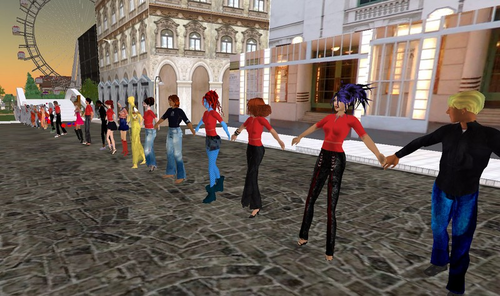
\includegraphics[width=6.094cm,height=4.094cm]{image/listeChainee.png}}
\end{center}

	\marginicon{objectif}
	Tout comme un tableau, une liste chainée est une collection d'éléments. 
	Mais, contrairement aux tableaux, les éléments ne sont pas contigus 
	en mémoire mais «~chainés~». Nous voyons ses avantages et inconvénients 
	par rapport aux tableaux, comment les implémenter en orienté-objet 
	et en non orienté-objet et les opérations de base sur les listes.


%=====================
\section{Définitions}
%=====================


	Voici quelques définitions de la liste chainée (\textit{linked list} 
	en anglais) issues de différents livres sur le
	sujet. Elles nous indiquent à la fois à quoi cela ressemble 
	et l'utilité d'une telle structure.
	
	\begin{itemize}
		\item 
			\textit{Une liste chainée désigne en informatique une structure de données
			représentant une collection ordonnée et de taille arbitraire d'éléments 
			de même type. L'accès aux éléments d'une liste se fait de manière 
			séquentielle~: chaque élément permet l'accès au suivant, 
			contrairement au cas du tableau dans lequel l'accès se fait de
			manière absolue, par adressage direct de chaque cellule 
			du dit tableau.} 
			(Wikipédia, août 2013)
		\item
			\textit{Une liste est un conteneur séquentiel capable d'insérer 
			et de supprimer des éléments localement de façon constante, 
			c'est-à-dire indépendamment de la taille du conteneur.} 
			(Structures de données en Java -- Hubbard -- ed. Schaum's)
	\item
		\textit{Les listes sont des conteneurs destinés aux insertions 
		s'effectuant en temps constant quelle que soit la position 
		dans le conteneur.} 
		(La bibliothèque standard STL du C++ -- Fontaine -- InterEditions)
	\item
		\textit{Une liste chainée est une structure de données dans 
		laquelle les objets sont arrangés linéairement. Toutefois,
		contrairement au tableau, pour lequel l'ordre linéaire est 
		déterminé par les indices, l'ordre d'une liste chainée est
		déterminé par un pointeur dans chaque objet.} 
		(Introduction à l'algorithmique -- Cormen, Leiserson, Rivest -- Dunod)
\end{itemize}


%===================================
\section{Liste versus liste chainée}
%===================================

	Dans la terminologie moderne, le terme \textit{liste} est 
	plutôt utilisé pour dénoter toute collection séquentielle
	d'éléments (il existe un premier élément, un deuxième {\dots}). 
	Autrement dit, chaque élément a une position précise dans
	la collection. En ce sens, un tableau ou un fichier sont 
	également des \textit{listes} !
	
	On peut opposer la liste à la structure d'\textit{ensemble} 
	où les éléments ne sont pas positionnés (un élément
	\textit{est} ou \textit{n'est pas} dans un ensemble mais 
	sans que sa position puisse être donnée).
	
	Le concept de liste ne doit pas être confondu avec la notion 
	de \textit{tri}. On peut parler de la \textit{liste}
	contenant les éléments 3, 8 et 2 dans cet ordre 
	(au sens de \textit{séquence} et pas d'\textit{ordre de tri}).


%=======================================
\section{Représentation et terminologie}
%=======================================

	Pour écrire explicitement une liste chainée et son contenu 
	sous forme compacte, on indique la liste des valeurs qu'elle
	contient entre parenthèses. Exemple~: la liste (3, 6, 5, 2).
	
	Schématiquement, on la représente plutôt ainsi~:

	\begin{center}
	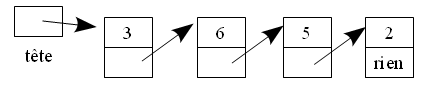
\includegraphics[width=11.324cm,height=2.355cm]{image/a2012Logique2eme-img002.png}
	\end{center}
	
	De ce schéma, il apparait que chaque \textbf{élément} 
	d'une liste chainée est composé de 2 parties~: la valeur
	proprement dite et un \textit{accès} à l'élément suivant. 
	De plus, on accède au premier élément de la liste via une
	zone spéciale, la \textbf{tête} de la liste chainée.

	Le dernier élément n'ayant pas de suivant, on indique \textit{rien} 
	dans la zone réservée à l'accès au suivant. Dans la
	littérature et selon les langages, on trouvera, à la place de \textit{rien}, 
	les notations \textit{null}, \textit{nil} {\dots} ou encore Ø.
	
	Le schéma ci-dessus peut encore se compactifier davantage, 
	en une forme qui ne fait pas apparaitre la tête de liste ni
	les accès aux éléments suivants~:

	\begin{center}
	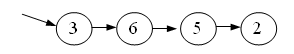
\includegraphics[width=7.779cm,height=1.429cm]{image/a2012Logique2eme-img003.png}
	\end{center}
	
	Au contraire du tableau, donc, il n'y a pas d'accès direct à un élément 
	(en donnant son indice) mais il est nécessaire
	de partir du premier élément et de suivre la «~\textit{chaine~»}. 
	Comment représenter ce \textit{lien}, cet
	\textit{accès} en mémoire ? Cela dépend du type de langage~:

	\begin{itemize}
		\item
			en programmation procédurale (non orienté-objet), 
			on utilise la notion de pointeur (cf. le cours de C/C++) tout en
			montrant qu'il est même possible de s'en sortir avec un langage 
			qui ne dispose pas de la notion de pointeur (comme par exemple Cobol) ;
		\item
			en orienté-objet (OO), un élément est représenté par un objet 
			dont un attribut est une référence vers l'objet
			représentant l'élément suivant.
	\end{itemize}


%===========================================================
\section{Rappel~: opérations sur les tableaux et complexité}
%===========================================================

	Afin de mieux comprendre ce qu'apporte la liste chainée 
	par rapport au tableau, revoyons ce que «~coûte~» les opérations
	courantes sur les tableaux. Le tableau ci-dessous donne la complexité 
	(par l'algorithme le plus économique) des
	opérations élémentaires pour un tableau trié et non trié.

	\begin{center}
		\tablefirsthead{}
		\tablehead{}
		\tabletail{}
		\tablelasttail{}
		\begin{supertabular}{|m{5.511cm}|m{3.6139998cm}|m{3.631cm}|}
		\hline
		\bfseries Opération &
		\bfseries Tableau non trié &
		\bfseries Tableau trié\\
		\hline
		Ajout d'un élément &
		\centering{O(1)} &
		\centering\arraybslash{O($n$)}\\
		\hline
		{Suppression d'un élément} &
		\centering{O($n$)} &
		\centering\arraybslash{O($n$)}\\
		\hline
		{Recherche d'un élément} &
		\centering{O($n$)} &
		\centering\arraybslash{O($log_{2}n$)}\\
		\hline
		{Parcours} &
		\centering{O($n$)} &
		\centering\arraybslash{O($n$)}\\\hline
		\end{supertabular}
	\end{center}
	
	Pour rappel, la notation O($n$) indique que l'opération 
	prend un temps qui est proportionnel à $n$, la
	taille du tableau. La plupart des opérations sont de complexité 
	O($n$), par exemple, lors d'une suppression, il
	faut décaler des éléments pour boucher le trou qui est apparu. 
	Il en est de même pour un ajout dans un tableau trié. Si
	le tableau n'est pas trié, il est évident qu'on peut rajouter 
	l'élément en fin de tableau, ce qui est immédiat
	(complexité O(1)). Dans le cas d'un tableau trié, c'est 
	l'algorithme de recherche dichotomique qui permet de trouver
	rapidement un élément avec une complexité O($log_{2}n$).

%==================================================
\section{Ajout d'un élément dans une liste chainée}
%================================================== 

	Dans une liste chainée (qu'elle soit ordonnée ou non), 
	il n'est pas nécessaire de décaler des éléments pour un ajouter
	un. Reprenons la liste chainée de l'exemple ci-dessus 
	et ajoutons l'élément 8 entre le 6 et le 5~:

	\ Avant~: \ \ \ \ \ \ \ \ \ \ \ \ \ \ \ \ \ \ \ \ \ \ \ \ \ \ \ \ \ \ \ \ \ \ \ \ \ \ \ \ \ \ \ \ \ \ \ \ \ \ \ \ \ \ \ \ \ \ Après~:

	 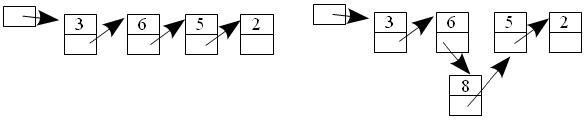
\includegraphics[width=15.558cm,height=3.334cm]{image/a2012Logique2eme-img004.png} 

	Il aura suffi de modifier des «~flèches~» (c'est-à-dire des «~liens~» 
	ou des «~accès~»). L'opération prend donc le même
	temps quelle que soit la taille de la liste chainée 
	(pour autant qu'on soit déjà positionné à l'endroit de l'ajout).

	La complexité de cette opération est donc O(1). Il n'y a ici pas de décalage d'éléments comme pour un tableau, pour la
	simple raison que les éléments d'une liste chainée n'ont aucune raison d'être à des endroits contigus dans la mémoire
	de l'ordinateur.

	Il y a un ajout qui fait figure de cas particulier, c'est l'ajout en tête de liste chainée, car il modifie
	obligatoirement l'accès au premier élément. Par exemple, si nous ajoutons 8 en première position, cela donne~:

	\ Avant~: \ \ \ \ \ \ \ \ \ \ \ \ \ \ \ \ \ \ \ \ \ \ \ \ \ \ \ \ \ \ \ \ \ \ \ \ \ \ \ \ \ \ \ \ \ \ \ \ \ \ \ \ \ \ \ \ \ \ Après~:

	 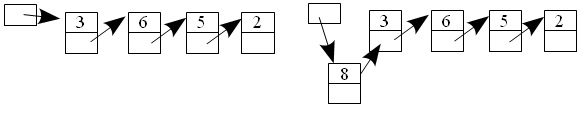
\includegraphics[width=15.452cm,height=3.122cm]{image/a2012Logique2eme-img005.png}
	
	
%========================================================
\section{Suppression d'un élément dans une liste chainée}
%========================================================
	
	La suppression d'un élément se fait tout aussi simplement. 
	L'opération est également de complexité O(1). Par exemple,
	supprimons l'élément de valeur 6~: 
	
	
	\ Avant~: \ \ \ \ \ \ \ \ \ \ \ \ \ \ \ \ \ \ \ \ \ \ \ \ \ \ \ \ \ \ \ \ \ \ \ \ \ \ \ \ \ \ \ \ \ \ \ \ \ \ \ \ \ \ \ \ \ \ Après~:

	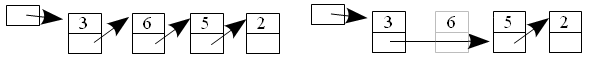
\includegraphics[width=15.61cm,height=1.773cm]{image/a2012Logique2eme-img006.png} 

	Ici aussi, le cas de la suppression du premier élément est particulier~:

	\ Avant~: \ \ \ \ \ \ \ \ \ \ \ \ \ \ \ \ \ \ \ \ \ \ \ \ \ \ \ \ \ \ \ \ \ \ \ \ \ \ \ \ \ \ \ \ \ \ \ \ \ \ \ \ \ \ \ \ \ \ Après~:

	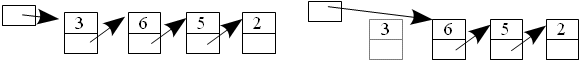
\includegraphics[width=15.425cm,height=1.72cm]{image/a2012Logique2eme-img007.png} 

	Remarquez que l'élément, quoique supprimé de la liste chainée, 
	est encore présent sur les schémas. Bien que l'élément ne
	fasse plus logiquement partie de l'ensemble des éléments 
	de la liste chainée, il est encore présent physiquement dans
	la mémoire. La suppression définitive de l'élément est gérée 
	soit par le programmeur lui-même, soit c'est le système
	qui nettoie de la mémoire les éléments auxquels plus aucun accès ne mène. 
	C'est le rôle du \textit{garbage collector},
	solution que nous avons adoptée en logique OO, 
	mais qui n'est pas vraie pour tous les langages OO (cf. C++).



%===============================
\section{Recherche d'un élément}
%===============================

	La recherche d'un élément dans une liste chainée non triée 
	est similaire à celle d'un tableau, il faut obligatoirement
	tout parcourir pour savoir si l'élément est présent ou non.

	Au contraire d'un tableau, le fait de savoir que la liste chainée 
	est triée (sur les valeurs des éléments) ne permet pas
	de développer un algorithme rapide de type \textit{recherche dichotomique}. 
	Tout au plus on peut, comme avec un tableau, s'arrêter lorsqu'on 
	dépasse la position où l'élément recherché aurait dû se trouver.


%=====================================
\section{Liste chainée versus tableau}
%=====================================

	Rajoutons dans le tableau ce que l'on a vu 
	de la complexité des listes chainées~:

	\begin{center}
		\tablefirsthead{}
		\tablehead{}
		\tabletail{}
		\tablelasttail{}
		\begin{supertabular}{|m{5.145cm}|m{2.023cm}|m{1.7329999cm}|m{2.836cm}|m{2.675cm}|}
		\hline
		{\bfseries Opération} &
		{\bfseries Tableau non trié} &
		{\bfseries Tableau trié} &
		{\bfseries Liste chainée non triée} &
		{\bfseries Liste chainée triée}\\
		\hline
		{Ajout d'un élément} &
		\centering{O(1)} &
		\centering{O($n$)} &
		\centering{O(1)} &
		\centering\arraybslash{O(1)}\\
		\hline
		{Suppression d'un élément} &
		\centering{O($n$)} &
		\centering{O($n$)} &
		\centering{O(1)} &
		\centering\arraybslash{O(1)}\\
		\hline
		{Recherche d'un élément} &
		\centering{O($n$)} &
		\centering{O($log_{2}n$)} &
		\centering{O($n$)} &
		\centering\arraybslash{ O($n$)}\\
		\hline
		{Parcours} &
		\centering{O($n$)} &
		\centering{O($n$)} &
		\centering{O($n$)} &
		\centering\arraybslash{O($n$)}\\
		\hline
		\end{supertabular}
	\end{center}
	
	On voit que la liste chainée montre tout son intérêt pour les ajouts 
	et les suppressions mais se montre moins efficace
	pour les recherches dans le cas où l'information est triée.

	Le choix d'un tableau ou d'une liste chainée pour représenter 
	une collection dans un problème précis dépend dès lors du
	rapport entre le nombre d'ajouts/suppressions et de recherches 
	que l'on compte effectuer.

	
	Remarquons aussi que dans le cas où les ajouts/suppressions se font 
	en \textit{fin} de tableau (le cas d'une \textit{pile} par exemple), 
	la complexité rejoint celle d'une liste chainée.

	Nous allons étudier l'implémentation de la liste chainée, 
	d'abord procédurale (ou \textit{«~C-like~»}) car c'est celle
	que vous utiliserez au labo C, ensuite nous verrons l'implémentation OO.


%===================================
\section{Implémentation procédurale}
%===================================

	\subsection{Notations}
	%=====================
	
	Pour les besoins de cette implémentation, nous devons introduire 
	une nouvelle notation~: l'\textbf{accès} à une
	variable, ou encore \textbf{référence} ou \textbf{pointeur}.

	La déclaration de cet accès se fera comme suit~:

	\cadre{
		\begin{pseudo}
			\Decl p~: accès à T
		\end{pseudo}
	}

	ce qui signifie que \textstyleCodeInsr{p} permet d'accéder à un élément 
	de type \textstyleCodeInsr{T}. 
	Dans le cadre de ce cours, comme les éléments d'une liste
	chainée peuvent être vus comme composés (structurés) d'un champ valeur 
	et d'un champ accès, nous n'aurons que des accès
	à des structures mais les langages non objets permettent généralement 
	des accès vers des éléments de type quelconque.

	Dans le contexte des références, il faut pouvoir créer dynamiquement 
	l'élément référencé. Cela s'indique par la
	primitive \textstyleCodeInsr{allouer}, à utiliser comme suit~:

	\cadre{
		\begin{pseudo}
			\Decl p \Gets \Alloc(T)
		\end{pseudo}
	}
	
	où \textstyleCodeInsr{T} est le type de l'élément référencé. 

	\textbf{Exemple}~: 
	\begin{pseudo}
		\Decl p \Gets \Alloc(Personne)
	\end{pseudo}
	
	Cette instruction provoque l'allocation d'un espace mémoire pour
	une variable de type \textstyleCodeInsr{Personne} et l'accès à 
	cet espace est placé dans \textstyleCodeInsr{p}. 
	En C, p pourrait être un pointeur recevant
	l'adresse de l'espace alloué lors de cette demande d'allocation.

	Pour accéder à la variable d'accès \textstyleCodeInsr{p}, 
	on utilisera la flèche vers la droite (comme en C), et donc,
	\cadre{
		\begin{pseudo}
			\Stmt p\Gives truc
		\end{pseudo}
	}
	
	désignera le champ \textit{truc} de la variable accessible par \textstyleCodeInsr{p}.

	
	Pour récupérer l'espace mémoire inutilement occupé par une variable 
	qui n'est plus utilisée, on a l'opération inverse
	qui se notera par la nouvelle primitive~:

	\cadre{
		\begin{pseudo}
			\Free p
		\end{pseudo}
	}
	
	qui supprime définitivement la variable d'accès \textstyleCodeInsr{p}, 
	ce qui a pour effet de rendre cet espace mémoire à nouveau
	allouable.

	Nous avons vu qu'un élément de liste est composé d'un champ \textit{valeur} 
	(qui contient la valeur proprement dite de
	l'élément) et d'un champ permettant d'accéder à l'élément suivant, 
	que nous nommerons simplement \textit{suivant}. Le
	type \textstyleCodeInsr{T} de la valeur de l'élément est noté entre crochets~:
	
	\cadre{
		\begin{pseudo}
			\Struct{ÉlémentListe<T>}
				\Decl valeur~: T
				\Decl suivant~: accès à ÉlémentListe<T>
			\EndStruct
		\end{pseudo}
	}
	
	\textbf{Exemple}~: pour un élément de liste chainée d'entiers, on définirait la structure~:
	
	\cadre{
		\begin{pseudo}
			\Struct{ÉlémentListe<entier>}
				\Decl valeur~: entier
				\Decl suivant~: accès à ÉlémentListe<entier>
			\EndStruct
		\end{pseudo}
	}
	
	En non orienté-objet, une liste chainée se reconnait simplement 
	par le fait que des éléments semblables (de même type)
	sont chainés, ce qui signifie que chacun d'eux contient un accès 
	à son suivant. Pour manipuler un tel ensemble de
	données, la seule condition est de pouvoir accéder au premier 
	élément de cet ensemble par une variable de type \textstyleCodeInsr{accès},
	que l'on peut appeler \textit{premier}, \textit{têteListe} ou encore 
	\textit{TL} (et qui n'a nul besoin d'être
	structurée). La liste chainée n'est donc rien d'autre qu'un accès, 
	celui au premier élément. Si cette liste est vide,
	cet accès a pour valeur \textit{rien}~:

	\cadre{
		\begin{pseudo}
			\Decl têteListe~: accès à ÉlémentListe<T> 
			\RComment accès au premier élément, rien si vide
		\end{pseudo}
	}

	\textbf{Exemple}~: pour déclarer une liste chainée d'entiers, on aurait~:

	\cadre{
		\begin{pseudo}
			\Decl têteListe~: accès à ÉlémentListe<entier>
		\end{pseudo}
	}

	\subsection{Exemple~1~: taille d'une liste chainée}
	%==================================================
	
		Voici un exemple d'algorithme calculant le nombre 
		d'éléments d'une liste chainée d'accès TL.
		
		\cadre{
			\begin{pseudo}
				\Module{tailleListeChainée}{TL~: accès à ÉlémentListe<T>}{entier}
					\Decl courant~: accès à ÉlémentListe<T>
					\Decl cpt~: entier
					\Let cpt \Gets 0
					\Let courant \Gets TL
					\While{courant ${\neq}$ rien}
						\Let cpt \Gets cpt + 1
						\Let courant \Gets courant\Gives suivant
					\EndWhile
					\Return cpt
				\EndModule
			\end{pseudo}
		}
			
	\subsection{Exemple~2~: mise d'un fichier en liste chainée}
	%==========================================================
		
		Dans ce 2\textsuperscript{e} exemple, on montre comment mettre 
		le contenu d'un fichier de variables structurées
		Identité (nom, prénom~: chaines, dateNais~: Date) dans une liste chainée.
		
		\cadre{
			\begin{pseudo}
				\Module{miseEnListe}{Personnes~: fichier de Identité}{accès à ÉlémentListe<Identité>}
					\Decl courant, précédent, TL~: accès à ÉlémentListe<Identité>
					\Decl enr~: Identité
					\Let TL \Gets rien 
					\RComment la liste est vide au départ
					\Stmt \K{ouvrir} Personne (\K{IN})
					\Read Personnes ; enr
					\If{NON EOF(Personnes)}
					\RComment traitement spécial pour le 1\textsuperscript{er} enregistrement
						\Decl TL \Gets \Alloc(ÉlémentListe<Identité>)
						\Decl TL\Gives valeur \Gets enr
						\Decl TL\Gives suivant \Gets rien
						\Decl précédent \Gets TL
						\Read Personnes ; enr
					\EndIf
					\While{NON EOF(Personnes)}
						\Decl courant \Gets \Alloc(ÉlémentListe<Identité>)
						\Decl courant\Gives valeur \Gets enr
						\Decl courant\Gives suivant \Gets rien
						\Decl précédent\Gives suivant \Gets courant
						\Decl précédent \Gets courant
						\Read Personnes ; enr
					\EndWhile
					
					\Stmt \K{fermer} Personnes
					\Return TL
				\EndModule
			\end{pseudo}
		}
		
		
%=====================================
\section{Représentation sans pointeur}
%=====================================

	La plupart des langages non orienté-objet possèdent la notion 
	de pointeur mais il y a des exceptions (Cobol par
	exemple). Comment implémenter une liste chainée dans un tel langage? 
	En simulant par exemple la liste chainée via un
	tableau qui contient 2 champs (la valeur de l'élément 
	et l'indice de l'élément suivant).

	\textbf{Exemple}~: la liste chainée (3, 6, 5, 2) 
	pourrait être donnée par le tableau suivant~:

	\begin{center}
		\tablefirsthead{}
		\tablehead{}
		\tabletail{}
		\tablelasttail{}
		\begin{supertabular}{|m{0.40900004cm}|m{0.403cm}|m{0.403cm}|m{0.403cm}|m{0.38200003cm}|}
		\multicolumn{1}{m{0.40900004cm}}{{\itshape 1}} &
		\multicolumn{1}{m{0.403cm}}{{\itshape 2}} &
		\multicolumn{1}{m{0.403cm}}{{\itshape 3}} &
		\multicolumn{1}{m{0.403cm}}{{\itshape 4}} &
		\multicolumn{1}{m{0.38200003cm}}{{\itshape 5}}\\\hline
		{ 2} &
		{ 6} &
		{ 3} &
		{ 5} &
		{ ?}\\
		\hline
		{ 0} &
		{ 4} &
		{ 2} &
		{ 1} &
		{ ?}\\
		\hline
		\end{supertabular}
	\end{center}

	À condition de savoir aussi où commencer, c'est-à-dire connaitre 
	l'indice du premier élément (le 3\textsuperscript{e}
	dans notre exemple). L'indice 0 indique la fin de la liste chainée. 
	Pour ajouter un élément, il suffit de l'ajouter en
	fin de tableau et d'adapter les indices sur la deuxième ligne. 
	La suppression est aussi aisée mais crée un «~trou~»
	qu'il faut pouvoir gérer (par exemple via une liste des places libres). 


%=====================================
\section{Implémentation orienté-objet}
%=====================================

	\subsection{implémentation}
	%==========================
		
		Pour l'implémentation OO, nous allons définir deux classes, 
		une pour un élément de liste chainée, et une autre pour la
		liste chainée elle-même.

		\cadre{
			\begin{pseudo}
				\Class{ÉlémentListe<T>}
					\Private
						\Decl valeur~: T
						\Decl suivant~: ÉlémentListe<T>
					\Public
						\ConstrSign{ÉlémentListe<T>}{val~: T, elt~: ÉlémentListe<T>}
						\ConstrSign{ÉlémentListe<T>}{val~: T}
						\RComment suivant à rien
						\MethodSign{getvaleur}{}{T}
						\MethodSign{setValeur}{val~: T}{}
						\MethodSign{getSuivant}{}{ÉlémentListe<T>}
						\RComment ne renvoie rien si pas de suivant
						\MethodSign{setSuivant}{elt~: ÉlémentListe<T>}{}
				\EndClass
			\end{pseudo}
		}
		
		\cadre{
			\begin{pseudo}
				\Class{ListeChainée<T>}
					\Private
						\Decl premier~: ÉlémentListe<T>
					\Public
						\ConstrSign{ListeChainée<T>}{}
						\LComment crée une liste vide
						\MethodSign{getPremier}{}{ÉlémentListe<T>}
						\MethodSign{estVide}{}{booléen}
						\MethodSign{insérerTête}{val~: T}{}
						\LComment insère en début de liste un nouvel élément de valeur val
						\MethodSign{insérerAprès}{elt~: ÉlémentListe<T>, val~: T)}{}
						\LComment insère un nouvel élément de valeur val après elt
						\MethodSign{supprimerTête}{}{}
						\LComment supprime le premier élément d'une liste chainée
						\MethodSign{supprimerAprès}{elt~:	ÉlémentListe<T>)}{}
						\LComment supprime l'élément qui suit elt
				\EndClass
			\end{pseudo}
		}

	\subsection{Remarques~:}
	%========================
			
		\begin{itemize}
			\item 
				Pour la classe ListeChainée, on pourrait envisager l'ajout d'autres 
				attributs pour accélérer certaines opérations. Par
				exemple, on pourrait définir comme attribut la taille de la liste 
				chainée, ce qui serait redondant puisqu'on peut la
				calculer en parcourant les éléments. On parle d'attribut 
				«~calculable~» pour indiquer un attribut qui contient une
				information qui pourrait être calculée à partir des autres attributs. 
				La pratique montre qu'il ne faut pas abuser de ce type d'attribut.
			\item 
				À votre avis, pourquoi n'y a t-il pas de méthode 
				\textsf{supprimer(elt~: ÉlémentListe)} qui supprime
				de la liste chainée l'élément donné en paramètre ? 
		\end{itemize}
	
		Nous détaillons à présent le contenu des constructeurs 
		et méthodes définies ci-dessus. 
		
		Pour la classe ÉlémentListe<T>~:
		
		\cadre{
			\begin{pseudo}
				\Constr{ÉlémentListe<T>}{val~: T, elt~: ÉlémentListe<T>}
					\Decl valeur \Gets val
					\Let suivant \Gets elt
				\EndConstr
			\end{pseudo}
		}
		
		\cadre{
			\begin{pseudo}
				\Constr{ÉlémentListe<T>}{val~: T}
					\Let valeur \Gets val
					\Let suivant \Gets rien
				\EndConstr
			\end{pseudo}
		}
		
		\cadre{
			\begin{pseudo}
				\Method{getvaleur}{}{T}
					\Return valeur
				\EndMethod
			\end{pseudo}
		}
		
		\cadre{
			\begin{pseudo}
				\Method{setValeur}{val~: T}{}
					\Let valeur \Gets val
				\EndMethod
			\end{pseudo}
		}
		
		\cadre{
			\begin{pseudo}
				\Method{getSuivant}{}{ÉlémentListe<T>}
					\Return suivant 
				\EndMethod
			\end{pseudo}
		}
		
		\cadre{
			\begin{pseudo}
				\Method{setSuivant}{elt~: ÉlémentListe<T>}{}
					\Let suivant \Gets elt
				\EndMethod
			\end{pseudo}
		}
		
		Passons à présent à la classe ListeChainée~:
		
		\cadre{
			\begin{pseudo}
				\Constr{ListeChainée<T>}{}
					\Let premier \Gets rien
				\EndConstr
			\end{pseudo}
		}
		
		\cadre{
			\begin{pseudo}
				\Method{getPremier}{}{ÉlémentListe<T>}
					\Return premier
				\EndMethod
			\end{pseudo}
		}
		
		\cadre{
			\begin{pseudo}
				\Method{estVide}{}{booléen }
					\Return premier = rien
				\EndMethod
			\end{pseudo}
		}
		
		\cadre{
			\begin{pseudo}
				\Method{insérerTête}{val~: T}{}
					\Decl elt~: ÉlémentListe<T>
					\Let elt \Gets \K{nouveau} ÉlémentListe<T>(val, premier)
					\Let premier \Gets elt
				\EndMethod
			\end{pseudo}
		}
		
		\cadre{
			\begin{pseudo}
				\Method{insérerAprès}{elt~: ÉlémentListe<T>, val~: T}{}
					\Decl eltAInsérer~: ÉlémentListe<T>
					\If{elt = rien}
						\K{erreur} «~insérer après rien est impossible~»
					\EndIf
					\Let eltAInsérer \Gets \K{nouveau} ÉlémentListe<T>(val, elt.getSuivant())
					\Stmt elt.setSuivant(eltAInsérer)
				\EndMethod
			\end{pseudo}
		}
		
		\cadre{
			\begin{pseudo}
				\Method{supprimerTête}{}{}
					\LComment Les lignes en italique sont nécessaires si la libération de
					\LComment l'espace inutilisé est à charge du programme (comme en C++)
					\textit{\Decl sauve~: ÉlémentListe<T>}
					\If{premier = rien}
						\Stmt \K{erreur} «~la liste est vide~»
					\EndIf
					\Let \textit{sauve} \Gets \textit{premier}
					\Let premier \Gets premier.getSuivant()
					\textit{\Free sauve}
				\EndMethod
			\end{pseudo}
		}

		\cadre{
			\begin{pseudo}
				\Method{supprimerAprès}{elt~: ÉlémentListe<T>}{}
					\LComment Les lignes en italique sont nécessaires si la libération de
					\LComment l'espace inutilisé est à charge du programme (comme en C++)
					\textit{\Decl sauve~: ÉlémentListe<T>}
					\If{elt = rien}
						\Stmt \K{erreur} «~élément inexistant~»
					\Else
						\If{elt.getSuivant( ) = rien}
							\Stmt \K{erreur} «~pas de suivant~»
						\EndIf
					\EndIf
					\Let \textit{sauve} \Gets \textit{elt.getSuivant()}
					\Stmt elt.setSuivant(elt.getSuivant().getSuivant())
					\textit{\Free sauve}
				\EndMethod
			\end{pseudo}
		}
		

%=============================================
\section{Exemple~: taille d'une liste chainée}
%=============================================

	Pour exemple, réécrivons en OO le module calculant la taille d'une liste chainée.

	\cadre{
		\begin{pseudo}
			\Module{tailleListeChainée}{maListe~: ListeChainée<T>}{entier}
				\Decl courant~: ÉlémentListe<T>
				\Decl cpt~: entier
				\Let cpt \Gets 0
				\Let courant \Gets maListe.getPremier( )
				\While{courant ${\neq}$ rien}
					\Let cpt \Gets cpt + 1
					\Let courant \Gets courant.getSuivant( )
				\EndWhile
				\Return cpt
			\EndModule
		\end{pseudo}
	}


%====================
\section{Commentaire}
%====================

	Dans l'implémentation procédurale, nous aurions pu plagier complètement 
	la version OO où 2 classes ont été définies (ListeChainée et ÉlémentListe), 
	il aurait fallu 2 structures correspondantes et les modules correspondants 
	aux constructeurs et méthodes. Ceci a été fait pour ÉlémentListe mais pas 
	pour ListeChainée. À votre avis, pourquoi ?

	Il existe quelques variantes à la liste chainée, notamment la 
	\textit{liste bidirectionnelle} et la \textit{liste circulaire}.


%===============================
\section{Liste bidirectionnelle}
%===============================

	Dans une \textbf{liste bidirectionnelle}, chaque élément possède, 
	en plus d'une référence à l'élément suivant,
	une référence à l'élément \textit{précédent}. Un des avantages est 
	de faciliter grandement la suppression car il n'est
	plus nécessaire de connaître l'élément précédent pour pouvoir le faire 
	puisqu'on peut le retrouver à partir de
	l'élément à supprimer.

	Comme les liens entre les éléments permettent de se déplacer 
	dans les deux sens, il est logique qu'à la tête de liste
	corresponde une fin de liste (ou queue de liste). Schématiquement~:

	\begin{center}
	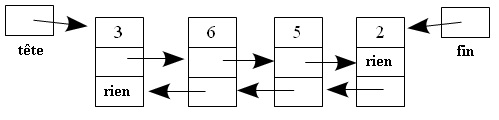
\includegraphics[width=13.203cm,height=3.175cm]{image/a2012Logique2eme-img008.png}
	\end{center}
	
	On peut facilement construire les classes ÉlémentListeBD et ListeBD 
	en adaptant légèrement les classes pour la liste
	chainée simple. La classe ListeBD aura comme attributs les deux accès 
	aux extrémités de la liste, nommés
	\textit{premier} et \textit{dernier}.
	
	\cadre{
		\begin{pseudo}
			\Class{ÉlémentListeBD<T>}
				\Private
					\Decl valeur~: T
					\Decl suivant~: ÉlémentListeBD<T>
					\Decl précédent~: ÉlémentListeBD<T>
				\Public
					\ConstrSign{ÉlémentListeBD<T>}{val~: T, suiv, prec~: ÉlémentListeBD<T>}
					\ConstrSign{ÉlémentListeBD<T>}{val~: T}
					\RComment précédent et suivant à rien
					\MethodSign{getvaleur}{}{T}
					\MethodSign{setValeur}{val~: T}{}
					\MethodSign{getSuivant}{}{ÉlémentListeBD<T>}
					\RComment ne renvoie rien si pas de suivant
					\MethodSign{setSuivant}{elt~: ÉlémentListeBD<T>}{}
					\MethodSign{getPrécédent}{}{ÉlémentListeBD<T>}
					\RComment ne renvoie rien si pas de précédent
					\MethodSign{setPrécédent}{elt~: ÉlémentListeBD<T>}{}
			\EndClass
		\end{pseudo}
	}
	
	\cadre{
		\begin{pseudo}
			\Class{ListeBD<T>}
				\Private
					\Decl premier~: ÉlémentListeBD<T>
					\Decl dernier~: ÉlémentListeBD<T>
				\Public
					\ConstrSign{ListeBD<T>}{}
					\MethodSign{getPremier}{}{ÉlémentListeBD<T>}
					\MethodSign{getDernier}{}{ÉlémentListeBD<T>}
					\MethodSign{estVide}{}{booléen}
					\MethodSign{insérerTête}{val~: T}{}
					\MethodSign{insérerFin}{val~: T}{}
					\MethodSign{insérerAprès}{elt~:	ÉlémentListeBD<T>, val~: T)}{}
					\MethodSign{insérerAvant}{elt~:	ÉlémentListeBD<T>, val~: T)}{}
					\MethodSign{supprimerTête}{}{}
					\MethodSign{supprimerFin}{}{}
					\MethodSign{supprimer}{elt~: ÉlémentListeBD<T>)}{}
			\EndClass
		\end{pseudo}
	}
	

%=========================
\section{Liste circulaire}
%=========================

	Dans une \textbf{liste circulaire}, le dernier élément ne référence 
	pas «~rien~» mais indique le premier élément.
	Schématiquement~:

	\begin{center}
	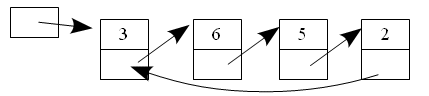
\includegraphics[width=11.351cm,height=2.54cm]{image/a2012Logique2eme-img009.png}
	\end{center}
	
	Il n'est pas nécessaire de créer une classe nouvelle pour les 
	éléments de la liste circulaire, puisqu'ils sont
	identiques à ceux d'une liste chainée simple. On peut faire fonctionner 
	ce type de liste avec les outils développés
	pour la liste chainée, il faut simplement veiller ici à la cohérence 
	de la liste circulaire, c'est-à-dire qu'à tout
	moment le dernier élément doit être lié au premier. Notez que premier 
	a ici un sens différent du point de vue logique,
	dans une liste circulaire il n'y a pas réellement de \textit{premier} 
	élément, mais un accès à un élément quelconque de
	la liste, peu importe sa position.
	
	
%==================
\section{Exercices}
%==================

	{\bfseries
	Remarques préliminaires}

	\begin{itemize}
		\item 
			\textit{Dans les exercices qui suivent, vous serez souvent amenés à 
			écrire des algorithmes similaires dont le code ne diffère
			qu'en un seul endroit. Dans cette situation, il faut toujours se 
			demander s'il n'est pas possible de factoriser le
			code, c'est-à-dire de le rendre modulaire de façon à limiter 
			l'écriture de code semblable.}
		\item
			\textit{Dans les exercices sur les listes, on s'efforcera toujours 
			de trouver la méthode la plus efficace (éviter de parcourir
			inutilement la liste) et aussi la plus économique (éviter si possible 
			les nouvelles demandes d'allocation d'éléments si
			ce n'est pas nécessaire).}
		\item 
			\textit{Sauf si c'est précisé, les exercices peuvent se faire 
			indifféremment en OO ou non, ce qui laisse la possibilité de
			s'entraîner dans les deux notations.}
	\end{itemize}
	
	\begin{Exercice}{Opérations de base}
		Écrire, dans la syntaxe de l'implémentation procédurale objet, 
		les modules qui correspondent aux méthodes de la liste 
		chainée dans la représentation OO, c'est-à-dire~:

		\begin{enumerate}
			\item {
				un module qui vérifie si une liste chainée est vide}
			\item {
				un module qui insère en début de liste un nouvel élément de valeur \textbf{val}}
			\item {
				un module qui insère un nouvel élément de valeur \textbf{val} après celui d'accès p}
			\item {
				un module qui supprime le premier élément d'une liste chainée}
			\item {
				un module qui supprime l'élément qui suit celui d'accès \textbf{p}}
		\end{enumerate}
	\end{Exercice}
	
	\begin{Exercice}{Insertions, recherches et suppressions}
		
		Soit une liste chainée contenant des valeurs d'un type T quelconque. Écrire~:

		\begin{enumerate}
			\item {
				un module qui ajoute dans la liste un nouvel élément de valeur 
				\textbf{val} (à l'endroit qui permet le code le plus simple)}
			\item {
				un module qui recherche dans la liste la valeur \textbf{val} 
				et retourne l'accès à l'élément qui le contient (ou rien si
				la valeur ne s'y trouve pas). Si la valeur s'y trouve plusieurs 
				fois, le module en retourne la première occurrence.}
			\item {
				un module qui retourne un booléen indiquant si la liste 
				contient la valeur \textbf{val}}
			\item {
				un module qui supprime de la liste le premier élément contenant 
				une valeur \textbf{val}. Le module retournera un booléen
				indiquant si la suppression a été réalisée~: vrai si \textbf{val} 
				a été supprimé, et faux sinon (parce que la valeur ne
				s'y trouvait pas).}
			\item {
				un module qui supprime de la liste toutes les occurrences de la valeur 
				\textbf{val} et retourne le nombre de suppressions réalisées}
		\end{enumerate}
		
		{\itshape
		N.B.~: cet exercice peut être réalisé de trois façons~(1) en procédural 
		(2) en orienté objet (3) sous forme de méthodes de la classe ListeChainée}
	\end{Exercice}

	\begin{Exercice}{Le grand nettoyage}
		Soit une liste chainée dont les valeurs (non ordonnées) sont des 
		entiers compris entre 1 et 10 inclus. On demande
		d'écrire l'algorithme qui supprime de cette liste toutes les 
		occurrences de la valeur la plus fréquente. En cas
		d'\textit{ex-æquo}, c'est la plus grande des valeurs qui est éliminée.

		\textit{Exemple}~: la liste (8, 7, 6, 7, 7, 1, 7, 1, 5, 7) devient (8, 6, 1, 1, 5).
	\end{Exercice}

	\begin{Exercice}{Liste chainée ordonnée}
		Soit une liste chainée dont les éléments sont triés (les 
		éléments sont d'un type T non précisé, mais on suppose que les
		opérateurs de comparaison (<, >, ={\dots}) sont autorisés pour 
		ce type). Réécrire les modules de l'exercice 2 en effectuant 
		les changements optimisant le code et la performance.
	\end{Exercice}

	\begin{Exercice}{Pas de doublons}
		Soit une liste chainée dont les éléments sont triés (idem 
		que pour l'exercice précédent) mais \textbf{ne contenant pas
		de doublons}. Réécrire les modules de l'exercice 4 qui 
		nécessitent un changement ou une adaptation.
	\end{Exercice}

	\begin{Exercice}{Liste bidirectionnelle}
		Développer le code des méthodes introduites dans la classe ListeBD.
	\end{Exercice}
	
	\begin{Exercice}{Liste circulaire}
		Transformer la classe ListeChainée en ListeChainéeCirculaire, 
		en ne changeant que les méthodes qui nécessitent une
		adaptation. Ajouter dans cette classe une méthode qui calcule 
		la taille de la liste, et une méthode qui permet
		d'ajouter un élément de valeur donnée à l'emplacement qui 
		correspond au code le plus performant.
	\end{Exercice}

	\begin{Exercice}{Tassement de liste}
	
		Soit une liste chainée d'entiers dont les éléments sont ordonnés 
		en ordre croissant sur les valeurs, et dans laquelle
		plusieurs éléments consécutifs peuvent avoir la même valeur. 
		Écrire un algorithme qui supprime de cette liste toutes
		les valeurs redondantes.

		\textit{Exemple}~: la liste (5, 5, 7, 7, 7, 11, 13, 13, 15) devient (5, 7, 11, 13, 15)
	\end{Exercice}
	
	\begin{Exercice}{Inter-classement de listes}
		Soient deux listes chainées de même type d'éléments. On voudrait 
		créer à partir de celles-ci une liste chainée issue de
		l'inter-classement des éléments de ces deux listes, c'est-à-dire 
		contenant dans l'ordre le premier élément de la
		première liste, le premier élément de la seconde liste, 
		le 2\textsuperscript{e} élément de la première liste, le
		2\textsuperscript{e} élément de la seconde liste et ainsi de suite. 
		Si une des deux listes est plus longue, on
		rattache le reste de celle-ci à la fin de la liste obtenue par 
		l'inter-classement des premiers éléments.

		\textit{Exemple}~: l'inter-classement des listes (2, 5, 9, 8, 10) et 
		(7, 4, 3) donnera comme résultat la liste
		(2, 7, 5, 4, 9, 3, 8, 10)

		Réaliser cet exercice~:

		\begin{enumerate}
			\item {
				En créant une 3\textsuperscript{e} liste 
				(les deux listes de départ restent intactes)}
			\item {
				Sans nouvelle demande d'allocation d'élément, c'est-à-dire 
				en incorporant les éléments de la 2\textsuperscript{e}
				liste à la première.}
		\end{enumerate}
		
		N.B.~: \textit{si vous réalisez cet exercice en OO, vous aurez besoin 
		exceptionnellement d'une méthode } \textstyleCodeInsr{setPremier( )}
		\textit{ que nous n'avons pas introduite dans la classe ListeChainée, 
		son emploi étant assez rare.}
	\end{Exercice}
	
	\begin{Exercice}{Fusion de listes}
		Écrire un algorithme qui fusionne 2 listes chainées ordonnées 
		de même type d'éléments. Comme dans l'exercice précédent,
		on envisagera les cas où (a) c'est une nouvelle liste qui 
		est créée (b) la seconde liste est incorporée à la première
		sans nouvelle demande d'allocation d'élément.
	\end{Exercice}
	
	\begin{Exercice}{Tri-fusion par éclatement des monotonies croissantes}
		Soit une liste chainée à valeurs entières. Une monotonie croissante 
		est une suite d'éléments qui se suivent et dont les
		valeurs sont dans l'ordre croissant. Le tri-fusion consiste à extraire 
		une monotonie, puis une autre, et ainsi de
		suite, et de fusionner chaque monotonie extraite avec le résultat 
		des fusions précédentes. Après la dernière fusion, la
		liste obtenue sera ordonnée, et la liste initiale aura donc été 
		transformée en une liste triée. Réaliser l'algorithme.
	\end{Exercice}

	\begin{Exercice}{Les ensembles}
		Définissons une classe Ensemble représentant un ensemble d'entiers 
		(au sens mathématique du terme). Développer le code
		des constructeurs et méthodes.

		\cadre{
			\begin{pseudo}
				\Class{Ensemble}
					\Private
						\Decl valeurs~: ListeChainée<entier>
						\RComment les valeurs seront ordonnées 
					\Public
						\ConstrSign{Ensemble}{}
						\LComment crée un ensemble vide 
						\MethodSign{ajoute}{val~: entier}{}
						\LComment ajoute une valeur à l'ensemble 
						\MethodSign{contient}{val~: entier}{booléen}
						\LComment indique si l'ensemble contient la valeur 
						\MethodSign{union}{autreEnsemble~: Ensemble}{Ensemble}
						\LComment crée l'ensemble contenant tous les éléments des 2 premiers 
						\MethodSign{intersection}{autreEnsemble~: Ensemble}{Ensemble}
						\LComment crée l'ensemble des éléments communs aux 2 premiers 
						\MethodSign{différence}{autreEnsemble~: Ensemble}{Ensemble}
						\LComment retourne l'ensemble des éléments qui ne sont pas dans le 2\textsuperscript{e}ensemble 
				\EndClass
			\end{pseudo}
		}
	\end{Exercice}
	
	\begin{Exercice}{L'algorithme du survivant}
		Le jeu du survivant se déroule comme suit~: un nombre indéterminé de joueurs sont assis en cercle. Le meneur du jeu
		choisit un nombre entier au hasard (par ex. en lançant un dé) que nous appellerons le \textit{pas de décompte}.
		Ensuite, il parcourt le cercle de joueurs en tournant dans le sens horloger derrière eux tout en comptant une unité à
		chaque joueur rencontré, et ce jusqu'à ce que pas de décompte est atteint. Le joueur derrière lequel il s'arrête est
		alors éliminé, et le meneur recommence son décompte à partir du joueur restant suivant. Il recommence ceci jusqu'à ce
		qu'il ne reste plus qu'un seul joueur, qui est le «~survivant~» de ce jeu.

		Réaliser l'algorithme qui simule ce jeu. Les paramètres sont une liste chainée circulaire contenant les noms des
		joueurs, et le pas de décompte. On suppose que le premier élément auquel on accède dans la liste correspond au premier
		joueur compté par le meneur de jeu. L'algorithme retourne le nom du survivant.
	\end{Exercice}

	\begin{Exercice}{Polynôme}
	
		Vous vous rappelez, par votre cours de mathématique, 
		qu'un \textit{monôme} est une expression de la forme
		\textit{ax}\textit{n}, où \textit{a} 
		est le coefficient, \textit{x} la variable et \textit{n}
		l'exposant (ex.~: $3x^2$). Un \textit{polynôme} est alors 
		une somme de monômes (ex.~: $3x^4-x^2+2$)

		\textit{Représentation}~: convenons de représenter un monôme 
		comme une simple structure avec 2 champs~: le coefficient
		et l'exposant. Un polynôme sera alors représenté comme une 
		liste chainée de monômes triés en ordre décroissant sur
		l'exposant.

		\textit{Problème}~: écrire un module permettant d'additionner 2 polynômes 
		et un autre permettant de les soustraire.
	\end{Exercice}

	\begin{Exercice}{Matrice creuse}
		Une matrice creuse est une matrice où la plupart des éléments sont nuls. 
		On les rencontre beaucoup dans des problèmes
		physiques impliquant des systèmes linéaires. Représenter une telle 
		matrice par un tableau classique à 2 dimensions
		n'est efficace ni en terme d'espace mémoire (une matrice 
		1000 \textsf{x} 1000 va contenir un million de valeurs presque
		toutes nulles) ni en terme de temps de calcul (beaucoup de calculs 
		avec des 0). C'est pourquoi on utilise souvent dans
		ce cas là un maillage de listes (une liste par ligne et une liste 
		par colonne).

		\textit{Exemple}~: La matrice~:

		\begin{figure}
			\centering
			\begin{minipage}{2.388cm}
			\begin{flushleft}
			\tablefirsthead{}
			\tablehead{}
			\tabletail{}
			\tablelasttail{}
			\begin{supertabular}{|m{0.393cm}|m{0.393cm}|m{0.393cm}|m{0.41000003cm}|}
			\hline
			{ 4} &
			{ 0} &
			{ 0} &
			{ 7}\\
			\hline
			{ 0} &
			{ 9} &
			{ 0} &
			{ 0}\\
			\hline
			{ 0} &
			{ 0} &
			{ 0} &
			{ 2}\\
			\hline
			\end{supertabular}
			\end{flushleft}
			\end{minipage}
		\end{figure}
		
		\bigskip
		
		\bigskip
		
		\bigskip
		
		sera représentée comme le suggère le schéma suivant~:

		\begin{center}
		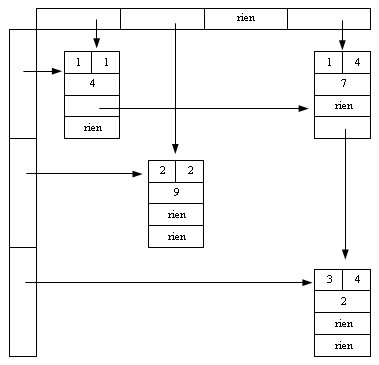
\includegraphics[width=10.028cm,height=9.657cm]{image/a2012Logique2eme-img010.png}
		\end{center}
		
		Chaque élément de la liste contient le numéro de ligne et 
		de colonne, la valeur, un lien vers l'élément non nul suivant
		dans la ligne et un lien vers l'élément non nul suivant dans 
		la colonne. On dispose également d'un tableau pour les
		têtes de lignes et un tableau pour les têtes de colonnes.

		On vous demande de~:

		\begin{enumerate}
			\item 
				Définir les attributs de la classe ÉlémentMatriceCreuse représentant un élément de la matrice.
			\item 
				Définir les attributs de la classe MatriceCreuse ainsi que
		
				\cadre{
					\begin{pseudo}
						\ConstrSign{MatriceCreuse}{nbLignes, nbColonnes~: entiers}
						\LComment construit une matrice vide
						\MethodSign{get}{ligne, col~: entiers}{entier}
						\LComment donne la valeur de l'élément de la matrice en position (ligne, col)
						\MethodSign{set}{ligne, {dots}, valeur~: entiers}{}
						\LComment affecte une valeur à l'élément de la matrice en position (ligne, col);
						\LComment si la valeur est nulle il faudra peut-être supprimer un élément;
						\LComment au contraire, si la valeur est non nulle, il faudra peut-être en ajouter.
					\end{pseudo}
				}
		\end{enumerate}
	\end{Exercice}


%%=========================
\chapter{La pile}
%=========================


%===================
\section{Définition}
%===================
	
	\marginicon{pile}	
	Une \textbf{pile} est une collection d'éléments admettant 
	les fonctionnalités suivantes~:

	\begin{itemize}
		\item {
			on peut toujours ajouter un élément à la collection;}
		\item {
			seul le dernier élément ajouté peut être consulté ou enlevé;}
		\item {
			on peut savoir si la collection est vide.}
	\end{itemize}

	La pile (en anglais \textit{stack}) est donc une collection 
	de données de type \textit{dernier entré, premier sorti} (en
	anglais on dit «~LIFO~», c'est-à-dire \textit{last in first out}). 
	L'analogie avec la pile de dossiers sur un bureau
	est claire~: les dossiers sont déposés et retirés du sommet 
	et on ne peut jamais ajouter, retirer ou consulter un dossier 
	qui se trouve ailleurs dans la pile.
	
	\begin{center}
	
\includegraphics[width=7.553cm,height=4.357cm]{image/a2012Logique2eme-img012.jpg}
	\end{center}
	
	On ne peut donc pas parcourir une pile, ou consulter directement 
	le \textit{n}\textsuperscript{ème} élément. Les opérations permises
	avec les piles sont donc peu nombreuses, mais c'est précisément 
	là leur spécificité~: elles ne sont utilisées en
	informatique que dans des situations particulières où seules 
	ces opérations sont requises et utilisées. Paradoxalement,
	on implémentera une pile en restreignant des structures plus 
	riches aux seules opérations autorisées par les piles.
	
	Des exemples d'utilisations sont la gestion de la mémoire 
	par les micro-processeurs, l'évaluation des expressions
	mathématiques en notation polonaise inverse, la fonction 
	«~ctrl-Z~» dans un traitement de texte qui permet d'annuler
	les frappes précédentes, la mémorisation des pages web visitées 
	par un navigateur, etc. Nous les utiliserons aussi plus
	loin dans ce cours pour parcourir les arbres et les graphes.


%=====================================
\section{Implémentation orienté-objet}
%=====================================

	\subsection{Allure générale}
	%===========================
		
		Nous allons d'abord décrire l'allure générale de la 
		classe pile. Nous ne précisons pas encore les détails de
		l'implémentation, plusieurs possibilités existent, 
		que nous détaillerons à titre d'exercice.

		\cadre{
			\begin{pseudo}
				\Class{Pile<T>}
				\RComment T est le type des éléments de la pile
					\Private 
						\LComment {à détailler plus tard}
					\Public 
						\ConstrSign{Pile<T>}{}
						\RComment crée une pile vide
						\MethodSign{empiler}{élément~: T}{}
						\RComment ajoute un élément au sommet de la pile
						\MethodSign{sommet}{}{T}
						\RComment retourne la valeur de l'élément au sommet de la pile, sans le retirer
						\MethodSign{dépiler}{}{T}
						\RComment enlève et retourne l'élément au sommet
						\MethodSign{estVide}{}{booléen}
						\RComment indique si la pile est vide
				\EndClass
			\end{pseudo}
		}
		
	\subsection{Remarques~:}
	%=======================
		
		\begin{itemize}
			\item 
				Théoriquement, et dans la majorité des utilisations, la pile 
				est \textit{infinie}, c'est-à-dire qu'on peut y ajouter un
				nombre indéterminé d'éléments (comme c'était le cas pour la 
				classe Liste étudiée en 1\textsuperscript{ère} année). Dans
				certaines situations, on peut cependant imposer une capacité 
				maximale à la pile (en pratique, c'est le cas de la pile
				de dossiers dans un bureau, elle est forcément limitée par 
				la hauteur du plafond !). Nous aborderons ce cas particulier
				dans les exercices.
			\item 
				Lors de l'implémentation de la classe, il faudra songer à envoyer 
				un message d'erreur lorsqu'on utilise les méthodes
				\textit{sommet} et \textit{dépiler} si la pile est vide. 
				Si la pile possède une taille maximale, alors c'est
				\textit{empiler} qui doit générer un message d'erreur 
				lorsque la pile est pleine.
			\item
				Nous avons utilisé ici des noms de méthodes neutres indépendants 
				de tout langage de programmation. Dans la littérature
				anglaise, on trouvera souvent \textit{push}, \textit{top} et 
				\textit{pop} en lieu et place de \textit{empiler},
				\textit{sommet} et \textit{dépiler}.
		\end{itemize}
		

%==============================
\section{Exemple d'utilisation}
%==============================

	Afin d'illustrer l'utilisation de la classe Pile, nous donnons 
	pour exemple un algorithme qui lit une suite d'enregistrements d'un 
	fichier \textbf{fileIn} (de type \textbf{Info}) et les reproduit en 
	ordre inverse dans le fichier \textbf{fileOut}.
	
	\cadre{
		\begin{pseudo}
			\Module{inverserOrdre}{fileIn\In~: FichierEntrée d'Info, fileOut\Out~: FichierSortie d'Info}{}
				\Decl enr~: Info
				\Decl pile~: Pile<Info>
				\LComment {1\textsuperscript{ère} étape~: parcours du fichier et mise en pile}
				\Let pile \Gets \K{nouveau} Pile<Info>
				\Stmt fileIn.ouvrir( )
				\Let enr \Gets fileIn.lire( )
				\While{NON fileIn.EOF( )}
					\Stmt pile.empiler(enr)
					\Let enr \Gets fileIn.lire( )
				\EndWhile
				\Stmt fileIn.fermer( )
				\LComment{2\textsuperscript{ème} étape~: vider la pile et écrire les éléments dans le fichier de sortie}
				\Stmt fileOut.ouvrir( )
				\While{NON pile.estVide( )}
					\Let enr \Gets pile.dépiler( )
					\Stmt fileOut.écrire(enr)
				\EndWhile
				\Stmt fileOut.fermer( )
			\EndModule
		\end{pseudo}
	}
	
	
%==================
\section{Exercices}
%==================

	\begin{Exercice}{Implémentation via une liste chainée}
		
		Détaillez l'implémentation de la classe pile en utilisant 
		comme attribut privé une liste chainée. Veillez à utiliser les
		méthodes qui permettent la gestion la plus efficace.
	\end{Exercice}

	\begin{Exercice}{La pile de taille finie}
		
		On envisage ici une pile dont la capacité est limitée~: elle 
		ne peut contenir au plus qu'un nombre donné d'éléments. On
		demande d'implémenter ce type de pile en utilisant un tableau. 
		Les attributs privés de la classe seront les suivants~:
		
		\cadre{
			\begin{pseudo}
				\Class{Pile<T>}
					\Private
						\Decl tab~: tableau de T 
						\RComment tableau (dynamique) contenant les éléments de la pile
						\Decl indSommet~: entier
						\RComment indice du sommet de la pile
						\Decl tailleMax~: entier
						\RComment taille maximale de la pile
					\EndClass
			\end{pseudo}
		}
		
		On remplira le tableau en ajoutant les éléments les uns à la 
		suite des autres et en retenant la position du dernier
		élément, qui correspondra à la valeur de l'attribut \textbf{indSommet}. 
		Cet attribut augmentera lorsqu'on ajoute un
		élément, et va décroître lorsqu'on en retire un.

		Détaillez l'implémentation des méthodes de la classe pile 
		correspondant à cette situation. Il faudra aussi
		adapter le constructeur, en lui donnant comme paramètre 
		la taille maximale de la pile.
	\end{Exercice}
	
	\begin{Exercice}{L'itinéraire retour}
		
		Un fichier \textbf{aller} contient la description d'un itinéraire. 
		Chaque enregistrement du fichier est une structure \textbf{étape} 
		contenant les champs \textbf{ville} (chaine) et \textbf{km} (réel). 
		Écrire un algorithme qui crée le fichier \textbf{retour} qui contiendra 
		-- au même format que \textbf{aller} -- la description de l'itinéraire retour.

		\bigskip

		\textbf{Exemple~:}
		
		\bigskip
		
		\begin{center}
		\tablefirsthead{}
		\tablehead{}
		\tabletail{}
		\tablelasttail{}
		\begin{supertabular}{|m{4.5cm}|m{2.0cm}|m{4.5cm}|m{2.0cm}|}
		\multicolumn{1}{m{4.5cm}}{{\itshape aller}} &
		\multicolumn{1}{m{2.0cm}}{{\itshape }} &
		\multicolumn{1}{m{4.5cm}}{{\itshape retour}} &
		\multicolumn{1}{m{2.0cm}}{{\itshape }} \\
		
		\multicolumn{1}{m{4.5cm}}{{ Bruxelles}} &
		\multicolumn{1}{m{2.0cm}}{{ 0}} &
		\multicolumn{1}{m{4.5cm}}{{ Amsterdam}} &
		\multicolumn{1}{m{2.0cm}}{{ 0}}\\
		
		\multicolumn{1}{m{4.5cm}}{{ Antwerpen}} &
		\multicolumn{1}{m{2.0cm}}{{ 40}} &
		\multicolumn{1}{m{4.5cm}}{{ Utrecht}} &
		\multicolumn{1}{m{2.0cm}}{{ 50}}\\
		
		\multicolumn{1}{m{4.5cm}}{{ Breda}} &
		\multicolumn{1}{m{2.0cm}}{{ 100}} &
		\multicolumn{1}{m{4.5cm}}{{ Breda}} &
		\multicolumn{1}{m{2.0cm}}{{ 120}}\\
		
		\multicolumn{1}{m{4.5cm}}{{ Utercht}} &
		\multicolumn{1}{m{2.0cm}}{{ 170}} &
		\multicolumn{1}{m{4.5cm}}{{ Anterpen}} &
		\multicolumn{1}{m{2.0cm}}{{ 180}}\\
		
		\end{supertabular}
	\end{center}

\end{Exercice}


%%=========================
\chapter{La file}
%=========================

\begin{center}
	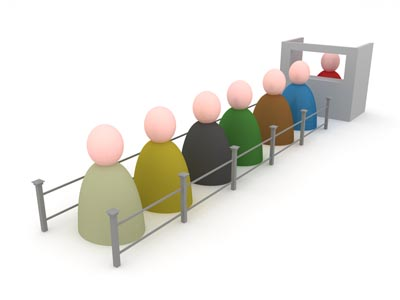
\includegraphics[width=7.553cm,height=4.357cm]{image/a2012Logique2eme-img013.jpg}
\end{center}
	

%===================
\section{Définition}
%===================
	
	\marginicon{file}	
	Une \textbf{file} est une collection d'éléments 
	admettant les fonctionnalités suivantes~:

	\begin{itemize}
		\item {
			on peut toujours ajouter un élément à la collection}
		\item {
			seul le premier élément ajouté peut être consulté ou enlevé}
		\item {
			on peut savoir si la collection est vide}
	\end{itemize}

	La file (en anglais \textit{queue}) est donc une collection 
	de données de type \textit{premier entré, premier sorti} 
	(en anglais on dit «~FIFO~», c'est-à-dire \textit{first in first out}). 
	L'analogie avec une file de clients à un guichet (poste, caisse du 
	supermarché, ...) est évidente~: c'est le premier arrivé qui est 
	le premier servi, et il est très malvenu d'essayer de doubler une personne 
	dans une file ! Noter qu'une fois entré dans une \textit{file} -- au
	sens informatique du terme -- on ne peut pas en sortir par l'arrière, 
	le seul scénario possible pour en sortir est
	d'attendre patiemment son tour et d'arriver en tête de la file.

	De même que pour la pile, on ne peut donc non plus parcourir une 
	file, ou consulter directement le \textit{n}\textsuperscript{ième}
	élément. Les files sont très utiles en informatique, citons par 
	exemple la création de mémoire tampon (\textit{buffer})
	dans de nombreuses applications, les processeurs multitâches 
	qui doivent accorder du temps-machine à chaque tâche, la
	file d'attente des impressions pour une imprimante, ...

%=====================================
\section{Implémentation orienté-objet}
%=====================================

	\subsection{Allure générale}
	%===========================
		
		Comme pour la pile, la classe File ne contient qu'un nombre 
		restreint de méthodes qui correspondent aux quelques
		opérations permises avec cette structure~: ajouter un élément 
		(\textit{«~enfiler~»}), consulter l'élément de tête, et
		le retirer (\textit{«~défiler~»}). Comme précédemment, nous ne 
		décrivons que les entêtes des constructeur et méthodes,
		le détail de l'implémentation sera laissé à titre d'exercices.

		\cadre{
			\begin{pseudo}
				\Class{File<T>}
				\RComment T est le type des éléments de la file
					\Private 
						\LComment {à détailler plus tard}
					\Public 
						\ConstrSign{File<T>}{}
						\RComment crée une file vide
						\MethodSign{enfiler}{élément~: T}{}
						\RComment ajoute un élément dans la file
						\MethodSign{tête}{}{T}
						\RComment retourne la valeur de l'élément en tête de file, sans le retirer
						\MethodSign{défiler}{}{T}
						\RComment enlève et retourne l'élément de tête
						\MethodSign{estVide}{}{booléen}
						\RComment indique si la file est vide
				\EndClass
			\end{pseudo}
		}
		
	\subsection{Remarques~:}
	%=======================
		
		\begin{itemize}
			\item 
				De même que dans le chapitre précédent, la file est supposée 
				\textit{infinie}, c'est-à-dire qu'on peut y ajouter un
				nombre indéterminé d'éléments. Le cas de la file limitée à 
				une capacité maximale sera envisagé dans l'exercice 2.
			\item
				Dans l'implémentation, il faudra songer à envoyer un message 
				d'erreur lorsqu'on utilise les méthodes \textit{tête} et
				\textit{défiler} si la file est vide. Si la file possède une 
				taille maximale, alors c'est \textit{enfiler} qui doit
				générer un message d'erreur lorsque la file est pleine.
		\end{itemize}

	
%==================
\section{Exercices}
%==================

	\begin{Exercice}{Implémentation via une liste chainée bidirectionnelle}
		
		Détaillez l'implémentation de la classe file en utilisant 
		comme représentation des données une liste chainée bidirectionnelle.
	\end{Exercice}

	\begin{Exercice}{La file de taille limitée}
		
		La file de taille limitée ne peut contenir au plus qu'un nombre d
		onné d'éléments. On demande d'implémenter ce type de
		file en utilisant un tableau. Les attributs privés de la 
		classe seront les suivants~:

		\cadre{
			\begin{pseudo}
				\Class{File<T>}
					\Private
						\Decl tab~: tableau de T 
						\RComment tableau (dynamique) contenant les éléments de la file
						\Decl premier~: entier
						\RComment indice du premier élément entré (tête de file)
						\Decl dernier~: entier
						\RComment indice du dernier élément entré (fin de file)
						\Decl tailleMax~: entier
						\RComment taille maximale de la file
					\EndClass
			\end{pseudo}
		}
				
		Nous proposons ici d'offrir un constructeur qui reçoit la 
		taille maximale de la file et qui crée un tableau d'indices 0
		à tailleMax (le tableau aura donc un élément de plus que 
		la taille maximale de la file, nous allons expliquer
		pourquoi). On remplit le tableau en ajoutant les éléments les 
		uns à la suite des autres en retenant la position du
		premier et du dernier via deux indices. Lorsqu'on ajoute un élément, 
		la position du dernier va augmenter, et lorsqu'on
		enlève un élément, cela revient à augmenter la position du premier, 
		afin d'éviter de devoir retasser l'ensemble de la
		file en début de tableau, ce qui serait une perte d'efficacité.

		\textbf{Exemple~:}

		Supposons qu'après la création de la file, les éléments 4, 3, 6 et 2 
		ont été ajoutés. L'indice du premier est 0 et celui du dernier est 3.

		\begin{center}
			\tablefirsthead{}
			\tablehead{}
			\tabletail{}
			\tablelasttail{}
			\begin{supertabular}{|m{1.171cm}|m{1.206cm}|m{1.206cm}|m{1.206cm}|m{1.206cm}|m{1.206cm}|m{1.206cm}|m{1.206cm}|m{1.206cm}|m{1.232cm}|}
			\hline
			\centering{\sffamily 4} &
			\centering{\sffamily 3} &
			\centering{\sffamily 6} &
			\centering{\sffamily 2} &
			~
			 &
			~
			 &
			~
			 &
			~
			 &
			~
			 &
			~
			\\\hline
			\end{supertabular}
		\end{center}
		
		On ajoute l'élément 7. L'indice du dernier est à présent 4.

		\begin{center}
			\tablefirsthead{}
			\tablehead{}
			\tabletail{}
			\tablelasttail{}
			\begin{supertabular}{|m{1.171cm}|m{1.206cm}|m{1.206cm}|m{1.206cm}|m{1.206cm}|m{1.206cm}|m{1.206cm}|m{1.206cm}|m{1.206cm}|m{1.232cm}|}
			\hline
			\centering{\sffamily 4} &
			\centering{\sffamily 3} &
			\centering{\sffamily 6} &
			\centering{\sffamily 2} &
			\centering{\sffamily 7} &
			~
			 &
			~
			 &
			~
			 &
			~
			 &
			~
			\\\hline
			\end{supertabular}
		\end{center}
		
		On enlève un élément de la file. L'indice du premier vaut maintenant 1

		\begin{center}
			\tablefirsthead{}
			\tablehead{}
			\tabletail{}
			\tablelasttail{}
			\begin{supertabular}{|m{1.171cm}|m{1.206cm}|m{1.206cm}|m{1.206cm}|m{1.206cm}|m{1.206cm}|m{1.206cm}|m{1.206cm}|m{1.206cm}|m{1.232cm}|}
			\hline
			~
			 &
			\centering{\sffamily 3} &
			\centering{\sffamily 6} &
			\centering{\sffamily 2} &
			\centering{\sffamily 7} &
			~
			 &
			~
			 &
			~
			 &
			~
			 &
			~
			\\\hline
			\end{supertabular}
		\end{center}
		
		Ce mécanisme peut se faire de façon circulaire~: arrivés en fin 
		de tableau, les indices premier et dernier repassent à
		0. Lorsque premier et dernier sont égaux, la file n'a qu'un 
		seul élément. Si cet élément est supprimé, l'incrémentation
		de premier aura pour conséquence que l'indice premier sera 
		d'une unité supérieur à l'indice dernier (en tenant compte
		de la rotation des valeurs), et ce sera donc la condition 
		correspondant à une file vide. Le tableau ne sera jamais
		rempli au maximum pour pouvoir distinguer le cas d'une file 
		vide et le cas d'une file pleine. Nous placerons donc dans
		le tableau au maximum tailleMax éléments (en laissant un 
		élément «~vide~» entre les indices dernier et premier).
	\end{Exercice}
	
	\begin{Exercice}{Le monte-charge}
		
		Un monte-charge de chantier assure le transport de personnes 
		et de matériel entre deux niveaux. Lorsque le monte-charge
		arrive à un étage, tous ses passagers en sortent. La charge
		maximale admise à la valeur MAX (donnée en paramètre).
		Étant donné les risques liés à l'utilisation du monte-charge 
		en surcharge, le poids de chacun des passagers et des
		charges qu'ils transportent (outils, brouette de sable, ...) 
		est vérifié avant l'entrée dans le monte-charge.

		Pour gérer l'embarquement dans le monte-charge, on souhaite 
		faire appel à un algorithme «~embarquement~» qui détermine
		combien de personnes qui se trouvent actuellement 
		en file devant le monte-charge peuvent y entrer.

		Cet algorithme respectera l'ordre d'arrivée des personnes 
		et mettra à jour la file des personnes en attente qu'il aura
		reçue en paramètre.

		\begin{enumerate}
			\item {
				Choisissez une représentation de données adaptée à la solution du problème et justifiez votre choix. }
			\item {
				Écrivez l'algorithme «~embarquement~»}
			\item {
				Écrivez l'algorithme «~arrivée~» qui ajoute à la file une personne d'un poids donné en paramètre.}
			\item {
				Quels cas doit-on envisager ?}
		\end{enumerate}

	\end{Exercice}

	\begin{Exercice}{À l'envers}
	
		Écrire un module recevant en paramètre une file d'entiers. 
		À l'issue de ce module, les valeurs de la file seront en
		ordre inverse et débarrassées des éléments pairs.

		\textbf{Exemple~:} Si le contenu de la file est le suivant~:

		{\centering
		1 $\rightarrow $ 0 $\rightarrow $ 4 
		$\rightarrow $ 25 $\rightarrow $ 20 
		$\rightarrow $ 11 $\rightarrow $ 3 $\rightarrow
		$ 7 $\rightarrow $ 8 $\rightarrow $ 73 
		$\rightarrow $ 2 $\rightarrow $ 4
		\par}

		son contenu sera après traitement~: 

		{\centering 
		73 $\rightarrow $ 7 $\rightarrow $ 3 $\rightarrow 
		$ 11 $\rightarrow $ 25 $\rightarrow $ 1
		\par}

\end{Exercice}
	
		
%%=========================
\chapter{L'association}
%=========================

\begin{center}
	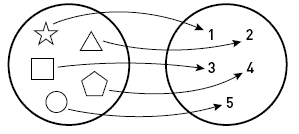
\includegraphics[width=5.66cm,height=2.536cm]{image/a2012Logique2eme-img014.png}
\end{center}
	

%=====================
\section{Introduction}
%=====================
	
	Dans ce chapitre, nous considérons des ensembles de données 
	possédant une \textbf{clé} (aussi appelée \textbf{identifiant}). 
	Par définition, la clé est unique pour chaque élément de l'ensemble. 
	Vous connaissez déjà de nombreux exemples par le cours de 
	bases de données, citons entre autres~:

	\begin{itemize}
		\item {
			le numéro d'étudiant, unique pour chaque étudiant de l'ESI}
		\item {
			le numéro de châssis d'un véhicule automobile}
		\item {
			le numéro de catalogue des produits vendus dans une grande surface}
		\item {
			le code postal des communes de Belgique, etc.}
	\end{itemize}

	Pour pouvoir stocker les éléments de ce type d'ensemble 
	dans le cadre de processus qui requièrent des accès fréquents
	aux données, nous devons recourir -- parmi les structures de 
	données vues jusqu'ici -- au tableau ou à la liste (la
	liste non chainée vue en 1\textsuperscript{ère} année). 
	L'inconvénient de ces structures réside dans le fait de devoir
	localiser les données par un indice, qui est dans la plupart 
	des cas un numéro d'ordre arbitraire qui n'est pas
	directement lié à la clé ; il faut donc toujours accompagner 
	la structure choisie d'un outil de recherche, ce qui
	implique un parcours des données pour chacune des opérations 
	de bases telles que la modification, la consultation ou la
	suppression d'un élément.

	Prenons l'exemple des étudiants de l'ESI dont l'identifiant 
	est un entier de 5 chiffres (par ex. 35421). Si on stocke
	les données dans un tableau par ordre alphabétique, il est 
	évident que l'indice de la case où se trouve un étudiant
	donné n'aura aucun rapport direct avec son numéro d'étudiant. 
	De même si on trie les données sur les numéros
	d'étudiant, rien ne permet de le localiser directement, 
	si ce n'est dans ce cas que la recherche pourrait être
	accélérée (par une recherche dichotomique par ex.). 
	On pourrait aussi envisager de placer un étudiant directement dans
	la case correspondant à son numéro d'étudiant (ainsi, l'étudiant 35421 
	serait dans la case 35421) mais ce n'est pas une
	idée très heureuse car elle exigerait d'utiliser un tableau 
	énorme dont la majorité des cases seraient inutilisées (il
	n'y a pas 35000 étudiants à l'ESI !) et de plus le tableau 
	contiendrait de nombreux trous (il n'y a pas un étudiant
	pour chacun des numéros dans un intervalle donné, certains 
	numéros disparaissent par exemple suite à un abandon).

	Nous allons dans ce chapitre construire une structure qui 
	permet de faire la liaison directe entre un élément et sa clé,
	et qui nous dispensera du problème «~technique~» de devoir 
	rechercher cet élément dans la structure. La connaissance de
	sa clé devrait permettre de le localiser immédiatement par 
	un algorithme de complexité minimale (en O(1) plutôt que en
	O(\textit{n})).


%===================
\section{Définition}
%===================

	Une \textbf{association} (on dit aussi \textit{dictionnaire} 
	ou encore \textit{map} selon la terminologie anglaise) lie
	des éléments à leur clé (ou identifiant). Il s'agit d'une 
	structure de données qui contient des couples (clé, valeur)
	et qui autorise les opérations suivantes~: stocker, retirer 
	et modifier un élément à partir de sa clé, connaitre le
	nombre d'éléments de l'ensemble (c'est-à-dire le nombre de 
	couples), et obtenir la liste des clés des éléments présents
	dans la structure.
	

%==================================
\section{Description orienté-objet}
%==================================

	Nous allons définir une classe Map (pour des raisons pratiques, 
	nous optons pour le nom anglais en raison de sa
	brièveté) dont les méthodes réalisent les opérations 
	citées ci-dessus. Les éléments contenus dans cette «~map~» sont
	des couples (clé, valeur). Plus précisément ce sont des variables 
	structurées dont les champs sont d'une part la clé
	(de type K, le plus souvent un entier ou une chaine de caractère) 
	et d'autre part la valeur (de type T quelconque). En
	particulier, la clé peut être elle-même un champ de la 
	valeur, ce qui peut paraitre redondant, mais nécessaire pour le
	fonctionnement de la classe.
	
	\cadre{
		\begin{pseudo}
			\Class{Map<K, T>}
			\LComment K est le type de la clé
			\LComment et T celui de la valeur
				\Private
					\LComment choix à détailler plus tard
				\Public 
					\ConstrSign{Map<K, T>}{...} 
					\RComment initialise la structure vide
					\MethodSign{setÉlément}{clé~: K, val~: T}{}
					\RComment ajoute le couple de clé donnée
					\MethodSign{getValeur}{clé~: K}{T}
					\RComment retourne la valeur associée à la clé
					\MethodSign{supprimer}{clé~: K}{}
					\RComment retire le couple associé à la clé
					\MethodSign{contient}{clé~: K}{booléen}
					\RComment indique si le couple de clé donnée est présent
					\MethodSign{taille}{}{entier}
					\RComment retourne le nombre de couples
					\MethodSign{listeClés}{}{Liste<K>}
					\RComment retourne la liste des clés présentes
			\EndClass
		\end{pseudo}
	}

	La méthode \textstyleCodeInsr{setÉlément} peut éventuellement 
	écraser une valeur précédente si la clé était déjà présente. 
	Les méthodes \textstyleCodeInsr{getValeur} et 
	\textstyleCodeInsr{supprimer} génèrent un message d'erreur si la clé en
	paramètre est absente de l'ensemble. La dernière méthode est 
	nécessaire pour pouvoir parcourir les éléments de l'ensemble. 
	En effet, sa structure interne étant un attribut privé inconnu 
	à l'extérieur de la classe, il est nécessaire d'avoir un outil 
	donnant la liste des clés présentes. En parcourant la liste et 
	en utilisant la méthode \textstyleCodeInsr{getValeur}, 
	on pourra ainsi passer en revue tous les éléments de l'association. 
	Il est à noter que la liste retournée n'est pas forcément dans 
	l'ordre des clés, c'est une limitation de cette structure.
	

%==============================
\section{Exemple d'utilisation}
%==============================

	Illustrons par un exemple l'utilité de la classe Map. Supposons qu'on
	veuille faire des statistiques sur les marques de voitures d'un grand 
	parc automobile. On voudrait connaitre le nombre de véhicules pour 
	chacune des marques présentes. Les données sont contenues dans un fichier 
	\textbf{fichAuto} dont chaque enregistrement de type Voiture contient 
	les champs \textbf{marque} (chaine), \textbf{modèle} (chaine),
	\textbf{immatriculation} (chaine), et d'autres données qui ne sont 
	pas utiles ici.
	
	Écrivons une première version sans utiliser la classe Map. 
	Nous avons besoin d'un compteur associé à chacune des marques de voitures. 
	Il est possible d'utiliser un tableau, mais avec l'inconvénient de ne 
	pas savoir à l'avance le nombre de marques différentes
	(ce qui pourrait se solutionner en déclarant le tableau avec une 
	taille raisonnablement grande dans ce contexte, 500 par exemple). 
	Nous allons plutôt opter pour une liste (classe Liste), 
	dont les éléments seront une structure \textbf{eltListe} 
	contenant les champs \textbf{marque} (chaine) et \textbf{cpt} (entier). 
	La démarche est simple~:
	lorsqu'une nouvelle marque est rencontrée, il faut ajouter un compteur 
	dans la liste initialisé à 1 ; si la marque a déjà été rencontrée, 
	il faut retrouver le compteur associé à cette marque et l'incrémenter. 
	Un module de recherche est donc indispensable pour le bon fonctionnement.

	\cadre{
		\begin{pseudo}
			\Module{statVoitures}{fichAuto\In~: fichier de Voiture}{}
				\Decl i, ind~: entier
				\Decl enr~: Voiture
				\Decl elt~: eltListe
				\Decl listeCpt~: Liste<eltListe>
				\Let listeCpt \Gets \K{nouveau} Liste<eltListe>( )
				\Stmt fichAuto.ouvrir( )
				\Let enr \Gets fichAuto.lire( )
				\While{NON fichAuto.EOF( )}
					\Let ind \Gets recherche(listeCpt, enr.marque)
					\If{ind = 0}
					\RComment la marque n'a pas encore été comptée
						\Let elt.marque \Gets enr.marque
						\Let elt.cpt \Gets 1
						\Stmt listeCpt.ajouter(elt)
					\Else
					\RComment la marque est présente dans la liste
						\Let elt\Gets listeCpt.get(ind)
						\Let elt.cpt \Gets elt.cpt + 1
						\Stmt listeCpt.set(ind, elt)
					\EndIf
					\Let enr \Gets fichAuto.lire( )
				\EndWhile
				\Stmt fichAuto.fermer( )
				\For{i \K{de} 1 \K{à} listeCpt.taille( )}
					\Write listeCpt.get(i).marque, listeCpt.get(i).cpt
				\EndFor
			\EndModule
		\end{pseudo}
	}
	
	\cadre{
		\begin{pseudo}
			\Module{recherche}{liste~: Liste<eltListe>, marque~: chaine}{entier}
			\LComment recherche dans la liste l'élément correspondant à la marque en paramètre
			\LComment et retourne sa position dans la liste, 0 s'il ne s'y trouve pas.
				\Decl i~: entier
				\Decl trouvé~: booléen
				\Let trouvé \Gets faux
				\Let i \Gets 0
				\While{NON trouvé ET i < liste.taille( )}
					\Let i \Gets i + 1
					\Let trouvé \Gets liste.get(i).marque = marque
				\EndWhile
				\If{trouvé}
					\Return i
				\Else 
					\Return 0
				\EndIf
			\EndModule
		\end{pseudo}
	}

	Avec la classe Map, le code se simplifie considérablement~: 
	nous sommes débarassés du module de recherche, et du souci
	de connaitre à quel endroit se trouve le compteur associé 
	à une marque donnée. Les valeurs seront ici les compteurs, et
	les clés les marques de voitures. On utilise donc une Map<chaine, entier>~:
	
	\cadre{
		\begin{pseudo}
			\Module{statVoitures}{FichAuto\In~: fichier de Voiture}{}
				\Decl enr~: Voiture
				\Decl i~: entier
				\Decl liste~: Liste<chaine>
				\Decl compteurs~: Map <chaine, entier>
				\Let compteurs \Gets \K{nouveau} Map<chaine, entier>( )
				\Stmt fichAuto.ouvrir( )
				\Let enr \Gets fichAuto.lire( )
				\While{NON fichAuto.EOF( )}
					\If{compteurs.contient(enr.marque)}
					\LComment la marque est déjà présente dans la Map
						\Stmt compteurs.setÉlément(enr.marque, compteurs.getValeur(enr.marque) + 1)
					\Else
					\LComment la marque n'est pas encore dans la Map
						\Stmt compteurs.setÉlément(enr.marque, 1)
					\EndIf
					\Let enr \Gets fichAuto.lire( )
				\EndWhile
				\Stmt fichAuto.fermer( )
				\Let liste \Gets compteurs.listeClés( )
				\For{i \K{de} 1 \K{à} liste.taille( )}
					\Write liste.get(i), compteurs.getValeur(liste.get(i))
				\EndFor
			\EndModule
		\end{pseudo}
	}
	
	
%=======================
\section{Implémentation}
%=======================

	On voit par l'exemple précédent que l'association apparait 
	de l'extérieur comme un ensemble non ordonné, une grande
	boite dans laquelle on introduit les couples (clé, valeur) 
	et de laquelle on peut les récupérer très facilement.
	Comment cela fonctionne-t-il ? Pour implémenter une association, 
	il est bien sûr possible d'utiliser les structures déjà connues~:

	\begin{itemize}
		\item {
			un tableau (trié ou non) ou une liste dont les éléments sont 
			les couples (clé, valeur) comme dans l'exemple des
			statistiques des marques de voitures}
		\item {
			une liste chainée (triée ou non)}
		\item {
			un arbre binaire ordonné sur les clés (voir chapitre sur les arbres)}
	\end{itemize}
	
	Utiliser une de ces structures comme attribut de la classe 
	reviendrait dès lors à camoufler à l'intérieur de la classe
	un algorithme de recherche tel que celui qui apparait explicitement 
	dans l'exemple ci-dessus, ce qui ne serait pas un
	réel progrès quant à l'efficacité.

	Il existe une structure particulière très efficace, nommée 
	\textit{table de hachage}, qui utilise un tableau pour
	stocker les éléments, et la position d'un élément dans ce 
	tableau se retrouve très rapidement en utilisant une
	\textit{fonction de hachage}.


%===============================
\section{La fonction de hachage}
%===============================

	Une \textit{fonction de hachage} transforme une clé 
	en un «~petit~» entier. Le but est d'obtenir par cette
	fonction (que nous noterons \textit{h}(\textit{x}) des 
	valeurs entre 1 (ou 0) et une valeur maximale \textit{n}, 
	et qui seront réparties le plus uniformément possible dans 
	cet intervalle. Le choix de la fonction de hachage dépend du 
	type de clé et aussi de la taille des éléments à classer.

	Cependant, il est courant que l'ensemble d'arrivée de la 
	fonction soit plus petit que l'ensemble des clés, et il est
	donc inévitable que deux clés différentes donnent le même 
	nombre après hachage. Dans ce cas on parle de «~collision~».
	Lors du choix de la fonction de hachage, il faut également 
	chercher à minimiser ces collisions, en vue d'un
	fonctionnement performant de la classe.

	\textbf{Exemples~:}

	\begin{itemize}
		\item {
			Prenons l'ensemble des étudiants de l'ESI, avec comme 
			clé le numéro d'étudiant de 5 chiffres. La fonction
			\textit{h}(\textit{x}) = \textit{x} DIV 1000 ne serait 
			pas un bon choix car elle donnerait un nombre réduit de valeurs
			(comprises actuellement entre 35 et 40), à partir d'un 
			ensemble de plusieurs centaines d'étudiants. La fonction
			\textit{h}(\textit{x}) = \textit{x} MOD 100 
			est déjà bien meilleure, elle donnerait des valeurs entre 0 et 99.
			Il y aura bien sûr des collisions, vu que les étudiants de 
			numéros 37156 et 38956 seraient «~hachés~» de la même façon.}
		\item {
			Pour les codes postaux des villes de Belgique, on pourrait 
			prendre la fonction \textit{h}(\textit{x}) = \textit{x} DIV 10. 
			Elle donnerait un ensemble de valeurs entre 100 et 999 
			où les collisions seraient peu nombreuses (vu que la plupart
			des codes se terminent par 0).}
	\end{itemize}


%============================
\section{La table de hachage}
%=============================

	La \textit{table de hachage} est un tableau contenant les couples 
	(clé, valeur) d'une association ; l'indice du tableau
	correspondant à un élément de clé donnée est déterminé par la 
	fonction de hachage \textit{h}(\textit{x}). Les valeurs
	de la fonction déterminent la taille du tableau (ou vice-versa). 
	Si la fonction de hachage donne des valeurs entre 1 et
	\textit{n}, il faudra un tableau de \textit{n} éléments.

	Pour les éléments de la table, nous définirons le type 
	structuré \textit{générique} suivant~:
	
	\cadre{
		\begin{pseudo}
			\Struct{Élément<K, T>}
				\Decl clé~: K
				\Decl valeur~: T
			\EndStruct
		\end{pseudo}
	}
	
	Par facilité de notation, nous admettrons par la suite la notation 
	\textstyleCodeInsr{(a, b)} pour désigner une variable de ce type, 
	avec \textstyleCodeInsr{a} et \textstyleCodeInsr{b} comme valeurs 
	respectives des champs clé et valeur.

	La table de hachage sera déclarée comme suit~:

	\cadre{
		\begin{pseudo}
			\Decl table~: tableau [1 à n] de Élément<K, T>
		\end{pseudo}
	}

	Pour stocker le couple (clé, valeur), nous écrirons donc~:

	\cadre{
		\begin{pseudo}
			\Let table[\textit{h}(clé)] \Gets (clé, valeur)
		\end{pseudo}
	}
	
	et pour trouver la valeur associée à une clé~:
	
	\cadre{
		\begin{pseudo}
			\Let val \Gets table[\textit{h}(clé)].valeur
		\end{pseudo}
	}

	\textbf{Exemple~:} 
	Dans cet exemple, seules les clés apparaissent, 
	nous faisons abstraction des valeurs. Prenons une
	table de capacité 10, pour y stocker des éléments déterminés 
	par des clés à valeurs entières. La fonction de hachage
	est \textit{h}(\textit{x}) = \textit{x} MOD 10 + 1. 
	Si les valeurs des clés à introduire dans la table sont 12, 17, 29
	et 33 on aura la configuration suivante~:

	\begin{center}
		\tablefirsthead{}
		\tablehead{}
		\tabletail{}
		\tablelasttail{}
		\begin{supertabular}{m{0.999cm}m{0.999cm}m{0.999cm}m{0.999cm}m{0.999cm}m{0.999cm}m{0.999cm}m{0.999cm}m{0.999cm}m{0.999cm}}
		\centering{\itshape 1} &
		\centering{\itshape 2} &
		\centering{\itshape 3} &
		\centering{\itshape 4} &
		\centering{\itshape 5} &
		\centering{\itshape 6} &
		\centering{\itshape 7} &
		\centering{\itshape 8} &
		\centering{\itshape 9} &
		\centering\arraybslash{\itshape 10}\\\hline
		\multicolumn{1}{|m{0.999cm}|}{~
		} &
		\multicolumn{1}{m{0.999cm}|}{~
		} &
		\multicolumn{1}{m{0.999cm}|}{\centering{ 12}} &
		\multicolumn{1}{m{0.999cm}|}{\centering{ 33}} &
		\multicolumn{1}{m{0.999cm}|}{~
		} &
		\multicolumn{1}{m{0.999cm}|}{~
		} &
		\multicolumn{1}{m{0.999cm}|}{~
		} &
		\multicolumn{1}{m{0.999cm}|}{\centering{ 17}} &
		\multicolumn{1}{m{0.999cm}|}{~
		} &
		\multicolumn{1}{m{0.999cm}|}{\centering\arraybslash{ 29}}\\\hline
		\end{supertabular}
	\end{center}
	
	Nous voyons aussi que l'occupation du tableau est irrégulière. 
	Il faut dès lors pouvoir reconnaitre les cases vides des
	cases occupées (par exemple en y mettant une valeur aberrante de la clé). 
	Que se passerait-il si on veut introduire la clé de valeur 42 ? 
	Elle devrait occuper la même case que 12, ce qui n'est pas possible. Nous sommes
	dans le cas d'une «~collision~» pour lequel nous envisageons deux solutions.


%===============================
\section{Gestion des collisions}
%===============================
	
	Il y a \textit{collision} entre deux clés 
	$k_1$ et k\textsubscript{2} lorsque
	\textit{h}(\textit{k}\textsubscript{1}) 
	= \textit{h}(\textit{k}\textsubscript{2}). 
	Que faire dans ces cas là ? Nous
	décrivons deux techniques courantes~: 
	l'«~adressage ouvert~» et le «~chainage~».

	\subsection{L'adressage ouvert}
	%==============================
		
		L'idée est la suivante~: lorsqu'on veut utiliser un emplacement 
		de la table et que celui-ci est occupé, on va voir
		ailleurs. Dans la technique la plus simple, on va simplement 
		continuer le parcours du tableau, à partir de la position
		de départ, à la recherche d'un «~trou~». Pour la recherche, 
		on procède de même; la fonction de hachage nous indique où
		commencer à chercher et on poursuit jusqu'à trouver 
		l'élément ou un «~trou~».

		Poursuivons l'exemple ci-dessus~: la clé 42 devrait occuper 
		la case d'indice 3. Comme celle-ci est occupée, on parcourt
		le tableau jusqu'à la prochaine case libre, celle d'indice 5 
		et on y place l'élément~:

		\begin{center}
			\tablefirsthead{}
			\tablehead{}
			\tabletail{}
			\tablelasttail{}
			\begin{supertabular}{m{0.999cm}m{0.999cm}m{0.999cm}m{0.999cm}m{0.999cm}m{0.999cm}m{0.999cm}m{0.999cm}m{0.999cm}m{0.999cm}}
			\centering{\itshape 1} &
			\centering{\itshape 2} &
			\centering{\itshape 3} &
			\centering{\itshape 4} &
			\centering{\itshape 5} &
			\centering{\itshape 6} &
			\centering{\itshape 7} &
			\centering{\itshape 8} &
			\centering{\itshape 9} &
			\centering\arraybslash{\itshape 10}\\\hline
			\multicolumn{1}{|m{0.999cm}|}{~
			} &
			\multicolumn{1}{m{0.999cm}|}{~
			} &
			\multicolumn{1}{m{0.999cm}|}{\centering{ 12}} &
			\multicolumn{1}{m{0.999cm}|}{\centering{ 33}} &
			\multicolumn{1}{m{0.999cm}|}{\centering{ 42}} &
			\multicolumn{1}{m{0.999cm}|}{~
			} &
			\multicolumn{1}{m{0.999cm}|}{~
			} &
			\multicolumn{1}{m{0.999cm}|}{\centering{ 17}} &
			\multicolumn{1}{m{0.999cm}|}{~
			} &
			\multicolumn{1}{m{0.999cm}|}{\centering\arraybslash{ 29}}\\\hline
			\end{supertabular}
		\end{center}
		
		Ce parcours de recherche est «~circulaire~»~: arrivé à la dernière case, 
		on revient au début. Ainsi, la clé 39 qui ne peut pas être mise 
		à sa place «~normale~» (occupée par 29) sera placée en première position~:

		\begin{center}
			\tablefirsthead{}
			\tablehead{}
			\tabletail{}
			\tablelasttail{}
			\begin{supertabular}{m{0.999cm}m{0.999cm}m{0.999cm}m{0.999cm}m{0.999cm}m{0.999cm}m{0.999cm}m{0.999cm}m{0.999cm}m{0.999cm}}
			\centering{\itshape 1} &
			\centering{\itshape 2} &
			\centering{\itshape 3} &
			\centering{\itshape 4} &
			\centering{\itshape 5} &
			\centering{\itshape 6} &
			\centering{\itshape 7} &
			\centering{\itshape 8} &
			\centering{\itshape 9} &
			\centering\arraybslash{\itshape 10}\\\hline
			\multicolumn{1}{|m{0.999cm}|}{\centering{ 39}} &
			\multicolumn{1}{m{0.999cm}|}{~
			} &
			\multicolumn{1}{m{0.999cm}|}{\centering{ 12}} &
			\multicolumn{1}{m{0.999cm}|}{\centering{ 33}} &
			\multicolumn{1}{m{0.999cm}|}{\centering{ 42}} &
			\multicolumn{1}{m{0.999cm}|}{~
			} &
			\multicolumn{1}{m{0.999cm}|}{~
			} &
			\multicolumn{1}{m{0.999cm}|}{\centering{ 17}} &
			\multicolumn{1}{m{0.999cm}|}{~
			} &
			\multicolumn{1}{m{0.999cm}|}{\centering\arraybslash{ 29}}\\\hline
			\end{supertabular}
		\end{center}
		
		L'exemple peut laisser perplexe vu la petite taille du tableau ; 
		si le tableau a une taille suffisante, on peut imaginer
		que la clé cherchée ne sera jamais très loin de la position 
		donnée par $h(x)$ de telle façon que la
		longueur du parcours requis peut être considéré comme négligeable.

		Noter que la suppression est plus délicate à mettre en {\oe}uvre~: 
		il ne suffit pas de supprimer simplement la clé dans
		la case donnée par la fonction de hachage, car s'il y a eu une 
		collision, on ne retrouverait plus l'autre valeur de clé. 
		Il faut donc reboucher le trou avec la dernière clé donnant 
		la même valeur de hachage. Ainsi, dans l'exemple, si
		on supprime 12, il faut déménager 42 dans la case d'indice 3~:
		
		\bigskip

		\begin{center}
			\tablefirsthead{}
			\tablehead{}
			\tabletail{}
			\tablelasttail{}
			\begin{supertabular}{m{0.999cm}m{0.999cm}m{0.999cm}m{0.999cm}m{0.999cm}m{0.999cm}m{0.999cm}m{0.999cm}m{0.999cm}m{0.999cm}}
			\centering{\itshape 1} &
			\centering{\itshape 2} &
			\centering{\itshape 3} &
			\centering{\itshape 4} &
			\centering{\itshape 5} &
			\centering{\itshape 6} &
			\centering{\itshape 7} &
			\centering{\itshape 8} &
			\centering{\itshape 9} &
			\centering\arraybslash{\itshape 10}\\\hline
			\multicolumn{1}{|m{0.999cm}|}{\centering{ 39}} &
			\multicolumn{1}{m{0.999cm}|}{~
			} &
			\multicolumn{1}{m{0.999cm}|}{\centering{ 42}} &
			\multicolumn{1}{m{0.999cm}|}{\centering{ 33}} &
			\multicolumn{1}{m{0.999cm}|}{~
			} &
			\multicolumn{1}{m{0.999cm}|}{~
			} &
			\multicolumn{1}{m{0.999cm}|}{~
			} &
			\multicolumn{1}{m{0.999cm}|}{\centering{ 17}} &
			\multicolumn{1}{m{0.999cm}|}{~
			} &
			\multicolumn{1}{m{0.999cm}|}{\centering\arraybslash{ 29}}\\\hline
			\end{supertabular}
		\end{center}
		
		Notons que la table a aussi une capacité maximale, on ne pourra 
		pas y mettre plus de clés que sa taille. Cette technique
		est donc assez délicate mais intéressante lorsque les allocations 
		dynamiques sont impossibles ou coûteuses. Si elles
		sont possibles, on utilisera plutôt la seconde technique~:

	\subsection{Le chainage}
	%=======================
		
		Avec cette technique, une entrée de la table ne contient 
		pas un couple (clé, valeur) mais une liste chainée de couples
		(clé, valeur)~: précisément tous les couples dont 
		les clés ont la même valeur de hachage.

		\cadre{
			\begin{pseudo}
				\Decl table~: tableau [1 à n] de ListeChainée<{Élément<K, T>}>
			\end{pseudo}
		}

		Pour rechercher un élément, il suffit à présent de parcourir 
		la liste chainée dont l'accès se trouve dans la case
		d'indice $h(x)$. L'avantage est l'aisance de 
		l'implémentation, moins délicate que l'adressage ouvert,
		et de plus, il n'y a pas de limitation (théorique) 
		au nombre de clés. Toutefois, il faut veiller à prendre un tableau
		assez grand pour que la taille des listes reste 
		réduite, le but étant de minimiser les parcours.

		Avec la technique de chainage, l'introduction des clés 
		12, 17, 29, 33, 42 et 39 dans la table donnerait la configuration
		suivante~:

		\begin{center}
			\tablefirsthead{}
			\tablehead{}
			\tabletail{}
			\tablelasttail{}
			\begin{supertabular}{m{0.999cm}m{0.999cm}m{0.999cm}m{0.999cm}m{0.999cm}m{0.999cm}m{0.999cm}m{0.999cm}m{0.999cm}m{0.999cm}}
			\centering{\itshape 1} &
			\centering{\itshape 2} &
			\centering{\itshape 3} &
			\centering{\itshape 4} &
			\centering{\itshape 5} &
			\centering{\itshape 6} &
			\centering{\itshape 7} &
			\centering{\itshape 8} &
			\centering{\itshape 9} &
			\centering\arraybslash{\itshape 10}\\\hline
			\multicolumn{1}{|m{0.999cm}|}{\centering{ rien}} &
			\multicolumn{1}{m{0.999cm}|}{\centering{ rien}} &
			\multicolumn{1}{m{0.999cm}|}{~
			} &
			\multicolumn{1}{m{0.999cm}|}{~
			} &
			\multicolumn{1}{m{0.999cm}|}{\centering{ rien}} &
			\multicolumn{1}{m{0.999cm}|}{\centering{ rien}} &
			\multicolumn{1}{m{0.999cm}|}{\centering{ rien}} &
			\multicolumn{1}{m{0.999cm}|}{~
			} &
			\multicolumn{1}{m{0.999cm}|}{\centering{ rien}} &
			\multicolumn{1}{m{0.999cm}|}{~
			}\\\hline
			~
			 &
			~
			 &
			\centering{ $\downarrow $} &
			\centering{ $\downarrow $} &
			~
			 &
			~
			 &
			~
			 &
			\centering{ $\downarrow $} &
			~
			 &
			\centering\arraybslash{ $\downarrow $}\\\hhline{~~--~~~-~-}
			~
			 &
			\multicolumn{1}{m{0.999cm}|}{~
			} &
			\multicolumn{1}{m{0.999cm}|}{\centering{ 42}} &
			\multicolumn{1}{m{0.999cm}|}{\centering{ 33}} &
			~
			 &
			~
			 &
			\multicolumn{1}{m{0.999cm}|}{~
			} &
			\multicolumn{1}{m{0.999cm}|}{\centering{ 17}} &
			\multicolumn{1}{m{0.999cm}|}{~
			} &
			\multicolumn{1}{m{0.999cm}|}{\centering\arraybslash{ 39}}\\\hhline{~~--~~~-~-}
			~
			 &
			~
			 &
			\centering{ $\downarrow $} &
			~
			 &
			~
			 &
			~
			 &
			~
			 &
			~
			 &
			~
			 &
			\centering\arraybslash{ $\downarrow $}\\\hhline{~~-~~~~~~-}
			~
			 &
			\multicolumn{1}{m{0.999cm}|}{~
			} &
			\multicolumn{1}{m{0.999cm}|}{\centering{ 12}} &
			~
			 &
			~
			 &
			~
			 &
			~
			 &
			~
			 &
			\multicolumn{1}{m{0.999cm}|}{~
			} &
			\multicolumn{1}{m{0.999cm}|}{\centering\arraybslash{ 29}}\\\hhline{~~-~~~~~~-}
			\end{supertabular}
		\end{center}

		(Il est évident que les ajouts se feront toujours en tête de liste).


%====================================
\section{Efficacité de la classe Map}
%====================================

	Comparons l'efficacité de plusieurs implémentations de la classe Map~: 
	le tableau (ordonné), la liste (non ordonnée),
	l'arbre binaire (ordonné) ou la table de hachage.

	\begin{center}
		\tablefirsthead{}
		\tablehead{}
		\tabletail{}
		\tablelasttail{}
		\begin{supertabular}{|m{3.3669999cm}|m{1.9679999cm}|m{1.8cm}|m{2.34cm}|}
		\hhline{~---}
		\multicolumn{1}{m{3.3669999cm}|}{~
		} &
		\centering{\bfseries recherche} &
		\centering{\bfseries ajout} &
		\centering\arraybslash{\bfseries suppression}\\\hline
		{\bfseries tableau} &
		\centering{O($log_{2}n$)} &
		\centering{O(\textit{n})} &
		\centering\arraybslash{ O(\textit{n})}\\\hline
		{\bfseries liste chainée} &
		\centering{O(\textit{n})} &
		\centering{O(\textit{n})} &
		\centering\arraybslash{O(\textit{n})}\\\hline
		{\bfseries arbre} &
		\centering{O($log_{2}n$)} &
		\centering{O($log_{2}n$)} &
		\centering\arraybslash{O($log_{2}n$)}\\\hline
		{\bfseries table de hachage} &
		\centering{O(1)} &
		\centering{O(1)} &
		\centering\arraybslash{O(1)}\\\hline
		\end{supertabular}
	\end{center}

	\textbf{Remarques}

	\begin{itemize}
		\item {
			La table de hachage est particulièrement efficace mais 
			ses performances se dégradent si la table est fort remplie à
			cause du nombre croissant de collisions, inconvénient que 
			n'a pas l'arbre.}
		\item {
			L'arbre sera étudié plus loin dans le cours ; signalons déjà 
			que c'est une structure qui a aussi l'avantage de permettre
			de donner facilement les éléments dans l'ordre des clés ce 
			que ne permet pas la table de hachage.}
	\end{itemize}



%==================
\section{Exercices}
%==================

	\begin{Exercice}{Hachage de clés entières}
		On stocke des valeurs associées à des clés entières 
		dans une table de hachage de capacité 15.
		La fonction de hachage est $h(x) = x MOD 15 + 1$. 
		Pour les deux techniques d'implémentations présentées 
		au cours (adressage ouvert et chainage), représenter 
		par un schéma l'état de la table
		après insertion dans l'ordre des clés suivantes~: 

		{\centering
		{17, 22, 36, 55, 21, 152, 64, 63, 10, 32}
		\par}

		Donner ensuite l'état de la table après suppression
		dans l'ordre des clés 55, 36 et 152.

	\end{Exercice}
	
	\begin{Exercice}{Hachage de chaines}
		On stocke des chaines de caractères dans une table de hachage 
		par la technique de l'adressage ouvert. La table permet de
		stocker 13 éléments et la fonction de hachage est donnée 
		par la formule $h(x) = 	(ordreAlphabet(initiale(\textit{x})) + 1) DIV 2$ 
		où \textbf{ordreAlphabet(car)} est la position dans l'alphabet du caractère car,
		et \textbf{initiale(chaine)} est le premier caractère de la chaine.
		
		Représenter le contenu de la table après exécution 
		dans l'ordre des actions suivantes~:

		\begin{itemize}
			\item {
				on ajoute «~André~», «~Edouard~», «~Francis~», «~Fabien~», «~Gilles~» et «~Geoffrey~»}
			\item {
				on retire «~Francis~» et «~Gilles~» }
			\item {
				on rajoute «~Arnaud~» et «~Francis~».}
		\end{itemize}

	\end{Exercice}
	
	\begin{Exercice}{Les membres}
		Un fichier Membres contient la liste des membres d'une association, 
		classés par ordre alphabétique sur leur nom. Chaque enregistrement est une 
		structure composée des champs \textbf{nom}, \textbf{prénom}, \textbf{rue}, 
		\textbf{numéro}, \textbf{ville}, \textbf{codePostal}, \textbf{dateNais}.

		Écrire un algorithme qui donne le nom de la ville 
		où habite le maximum de membres de l'association.

	\end{Exercice}
	
	\begin{Exercice}{Map avec chainage}
		Détailler l'implémentation de la classe Map à l'aide d'une 
		table de hachage fonctionnant avec la technique du chainage.
		On considère que la fonction de hachage $h(x)$ donne des 
		valeurs toujours comprises entre 1 et 1000.
	\end{Exercice}

	\begin{Exercice}{Gestion de stock}
		Soient la classe Article et la structure Achat définies comme suit~:
		
		\cadre{
			\begin{pseudo}
				\Class{Article}
					\Private
						\Decl code~: entier
						\Decl libellé~: chaine
						\Decl prix~: entier
						\Decl quantité~: entier
						
					\Public 
						\ConstrSign{Article}{unCode~: entier, unLibellé~: chaine, 
						unPrix~: entier, uneQuantité~: entier}
						\MethodSign{getLibellé}{}{chaine}
						\MethodSign{getCode}{}{entier}
						\MethodSign{getPrix}{}{entier}
						\MethodSign{getQuantité}{}{entier}
						\MethodSign{addQuantité}{q~: entier}{}
						\MethodSign{setPrix}{p~: entier)}{}
				\EndClass
			\end{pseudo}
		}
		
		\cadre{
			\begin{pseudo}
				\Struct{Achat}
					\Decl codeArticle~: entier
					\Decl quantité~: entier
				\EndStruct
			\end{pseudo}
		}

		Définissez la classe \textbf{Stock} pour qu'elle n'offre 
		que les méthodes suivantes que vous implémenterez. Veillez à
		choisir une implémentation des données assurant de bonnes performances.
		
		\cadre{
			\begin{pseudo}
				\MethodSign{màjStock}{articles~: Liste<Article>}{}
					\LComment articles reprend les articles de réapprovisionnement 
					du stock
					\LComment (nouveaux articles et/ou articles existants)
				\MethodSign{getQuantité}{code~: entier}{entier}
				\MethodSign{getLibellé}{code~: entier}{chaine}
				\MethodSign{getPrix}{code~: entier}{entier}
				\MethodSign{getCodesArticles}{}{Liste<entier>}
				\MethodSign{évaluer}{panier~: Liste<Achat>}{entier}
				\RComment retourne le prix total du panier
			\end{pseudo}
		}
	\end{Exercice}

%\include{log2-chapitre-récursivité}
%%=============================
\chapter{La structure d'arbre}
%=============================

{\itshape La structure d'arbre trouve de nombreuses utilités en informatique~: 
évaluation d'expressions algébriques, modélisation de l'inclusion d'ensembles,
d'organisations hiérarchiques, de schémas en analyse, d'arbre généalogique, 
arborescence des dossiers dans un système d'exploitation, variables 
structurées C et en Cobol {\dots}}
\begin{center}
	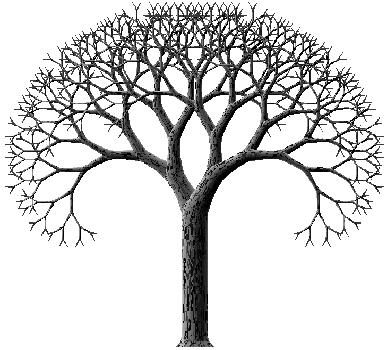
\includegraphics[width=4.494cm,height=4.045cm]{image/a2012Logique2eme-img028.png}
\end{center}
	

%===================================
\section{Définition et terminologie}
%===================================

	\subsection{arbre}
	%=================
		En informatique, un \textbf{arbre} est une structure de données 
		constituée de \textbf{n{\oe}uds} assemblés par \textbf{niveaux}. 
		C'est un graphe orienté connexe dont chaque arc relie un 
		\textbf{n{\oe}ud père} à un \textbf{n{\oe}ud fils}. 
		Chaque n{\oe}ud peut posséder un nombre quelconque de fils ; 
		un n{\oe}ud sans fils est appelé \textbf{n{\oe}ud terminal} 
		ou \textbf{feuille}.

		Chaque n{\oe}ud possède un et un seul père, sauf la \textbf{racine}, 
		située au sommet de l'arbre, qui ne possède pas de n{\oe}ud père. 
		Les n{\oe}uds autres que la racine ou les feuilles sont appelés 
		\textbf{n{\oe}uds internes}. Deux n{\oe}uds ayant le même père 
		sont des \textbf{frères}.

		\begin{center}
		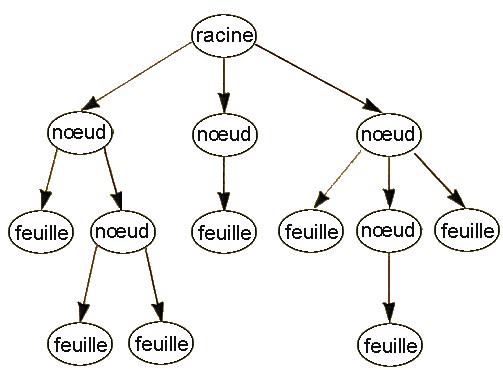
\includegraphics[width=9.036cm,height=6.636cm]{image/a2012Logique2eme-img029.png} 
		\end{center}
		
		\textit{Attention~: ne pas confondre l'arbre au sens informatique 
		et celui étudié dans la théorie des graphes au cours de mathématique ; 
		en théorie des graphes, un arbre est défini comme un graphe sans 
		circuit et est dépourvu de toute structure hiérarchique. L'arbre au sens
		informatique est aussi appelé arbre enraciné.}

		On peut aussi définir l'arbre de manière récursive~: 
		c'est une structure soit vide, soit composée d'un n{\oe}ud auquel
		est rattaché un ensemble fini d'arbres disjoints. 
		Notez que cette définition récursive correspond bien à la réalité de
		ce qu'est un arbre dans la nature !

	\subsection{Niveau et hauteur}
	%=============================

		Le \textbf{niveau} (ou \textbf{profondeur}) d'un n{\oe}ud 
		est la distance qui le sépare de la racine. Il en découle que
		le niveau de la racine est 0, et le niveau de tout autre 
		n{\oe}ud est égal au niveau de son père augmenté de 1.

		\begin{center}
		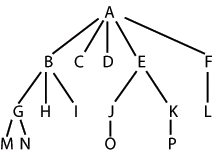
\includegraphics[width=5.092cm,height=3.819cm]{image/a2012Logique2eme-img030.png}
		\end{center}

		{\itshape	
		Exemple~: dans le graphe ci-dessus, les niveaux sont les suivants~: 
		0 pour A, 1 pour B, C, D, E, F, 2 pour G, H, I, J, K, L 
		et 3 pour M, N, O, P.}

		Inversement, la \textbf{hauteur} d'un n{\oe}ud est la distance entre 
		ce n{\oe}ud et sa descendance la plus éloignée~: la hauteur d'une 
		feuille est donc 0 et la hauteur de tout autre n{\oe}ud est le maximum 
		de la hauteur de ses fils augmenté de 1. La \textbf{hauteur d'un arbre} 
		est la hauteur de sa racine, et correspond aussi à son niveau maximum. 
		Elle n'est pas définie pour un arbre vide.

		{\itshape
		Pour le même graphe ci-dessus, les n{\oe}uds C, D, H, I, L, M, N, O et P 
		ont une hauteur 0 (ce sont les feuilles de l'arbre). 
		La hauteur de G, J, K et F est 1, celle de B et E est 2 
		et enfin A est à hauteur 3, qui correspond aussi à la hauteur de l'arbre.}

		Les n{\oe}uds d'un arbre contiennent de l'information, 
		appelée parfois «~étiquette~». L'étiquette peut être un simple
		entier ou une variable structurée plus complexe, l'instance 
		d'un objet, un pointeur, etc. Le type de l'information
		détermine le type de l'arbre~: on parlera d'un arbre 
		d'entiers, de chaines et en général d'arbre de type T.
	
	\subsection{Arbres particuliers}
	%===============================
	
		Un arbre dont tout n{\oe}ud possède au plus un descendant 
		est appelé \textbf{arbre dégénéré}.

		Un arbre dont tout n{\oe}ud possède au plus un nombre 
		déterminé \textit{n} de descendants est appelé \textbf{arbre
		}\textbf{\textit{n}-aire}. 
		
		Si dans un arbre \textit{n}-aire, toutes les feuilles ont 
		le même niveau, et si la racine et tous les n{\oe}uds
		internes ont le même nombre de fils, l'arbre est alors 
		\textbf{complet}. En particulier, un arbre dégénéré est complet ! 
		Le schéma ci-dessus montre un arbre «~2-aire~» complet~: 
		chaque n{\oe}ud non terminal à 2 fils, et toutes les
		feuilles sont au même niveau.

		\begin{center}
		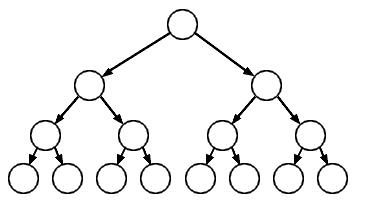
\includegraphics[width=6.918cm,height=3.909cm]{image/a2012Logique2eme-img031.png}
		\end{center}


%============================
\section{Parcours d'un arbre}
%============================

	Il y a plusieurs façons de parcourir un arbre, le choix du parcours 
	dépendant du type de traitement des informations de l'arbre.

	\subsection{Parcours en largeur}
	%===============================

		Le parcours en largeur, aussi nommé \textbf{parcours par niveau}, 
		consiste à visiter les n{\oe}uds dans l'ordre de leur niveau~: 
		la racine, puis les n{\oe}uds de niveau 1, ceux de niveau 2 
		et ainsi de suite. L'ordre de parcours des n{\oe}uds pour 
		un niveau donné est déterminé de manière récursive par 
		l'ordre des n{\oe}uds parents. Sur les schémas, l'ordre 
		des n{\oe}uds correspond à leur disposition de gauche à droite.

		{\itshape
		Exemple~: pour le graphe suivant, l'ordre de visite des n{\oe}uds 
		par le parcours par niveau est A, B, C, D, E, F, G, H,
		I, J, K, L, M, N, O, P.}

		\begin{center}
		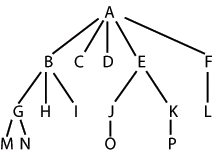
\includegraphics[width=5.821cm,height=4.366cm]{image/a2012Logique2eme-img032.png}
		\end{center}
	
	\subsection{Parcours en profondeur}
	%==================================
	
		Il s'agit d'un parcours récursif sur les n{\oe}uds de l'arbre~: 
		partant de la racine, on visite tous ses fils, mais on
			ne passe à un n{\oe}ud frère qu'après avoir visité tous les 
			fils du n{\oe}ud courant, et ceci récursivement. Il y a
			deux possibilités de traitement des n{\oe}uds~: si le 
			n{\oe}ud courant est traité avant ses fils, on parle de
			\textbf{parcours préfixé}. Si le n{\oe}ud courant est 
			traité après ses fils, on parle de \textbf{parcours postfixé}.

			{\itshape
			Pour le graphe ci-dessus, le parcours en profondeur préfixé donne~: 
			A, B, G, M, N, H, I, C, D, E, J, O, K, P, F, L. 
			Le parcours en profondeur postfixé donne~: 
			M, N, G, H, I, B, C, D, O, J, P, K, E, L, F, A.}
			

%=====================================
\section{Implémentation orienté objet}
%=====================================

	Un arbre est déterminé par sa racine qui est un n{\oe}ud de type T. 
	Chaque n{\oe}ud contient de l'information (attribut
	valeur de type T) et doit permettre de passer à ses 
	descendants (le 1\textsuperscript{er}, le 2\textsuperscript{e},
	etc.) d'où également un attribut de type Liste qui permet 
	d'accéder par position à chacun des fils (Liste d'éléments de
	type N{\oe}ud<T>). L'implémentation de l'arbre est donc 
	déterminée par la donnée des deux classes suivantes~: 
	
	\cadre{
		\begin{pseudo}
			\Class{N{\oe}ud<T>}
				\Private
					\Decl valeur~: T
					\Decl ListeFils~: Liste<{N{\oe}ud<T>}>
				\Public
					\ConstrSign{N{\oe}ud<T>}{val~: T}
					\LComment construit un n{\oe}ud sans fils
					\MethodSign{getValeur}{}{T}
					\MethodSign{setValeur}{val~: T}{}
					\MethodSign{getNbFils}{}{entier}
					\MethodSign{getFils}{i~: entier}{N{\oe}ud<T>}
					\MethodSign{setFils}{i~: entier, fils~: N{\oe}ud<T>}{}
					\MethodSign{ajouterFils}{fils~: N{\oe}ud<T>}{}
					\RComment ajout à la fin de la liste des fils
					\MethodSign{supprimerFils}{i~: entier}{}
			\EndClass
		\end{pseudo}
	}
	
	\cadre{
		\begin{pseudo}
			\Class{Arbre<T>}
				\Private
					\Decl racine : N{\oe}ud<T>
				\Public
					\ConstrSign{Arbre<T>}{}
					\LComment construit un arbre vide
					\MethodSign{getRacine}{}{N{\oe}ud<T>}
					\MethodSign{setRacine}{racine~: N{\oe}ud<T>}{}
			\EndClass
		\end{pseudo}
	}

	Les contenus des méthodes de la classe N{\oe}ud<T> se laissent 
	deviner aisément ; les cinq dernières méthodes consistent à appliquer 
	respectivement sur l'attribut \textbf{ListeFils} 
	les méthodes \textit{taille}, \textit{get}, \textit{set}, 
	\textit{ajouter} et \textit{supprimer} de la classe Liste.

	Noter que -- comme pour la liste chainée monodirectionnelle -- 
	on ne peut voyager dans un arbre que dans un seul sens,
	de la racine vers les feuilles, il n'y a pas de lien 
	d'un n{\oe}ud vers son n{\oe}ud père. Le rajout de ce lien serait
	une possibilité d'implémentation (comme pour la liste bidirectionnelle) 
	mais il n'est pas nécessaire pour la plupart des algorithmes 
	de parcours qui fonctionnent essentiellement de manière récursive 
	(pour les parcours en profondeur) ou à l'aide d'une file 
	(parcours en largeur). Nous donnons à titre d'exemple le détail 
	de ces algorithmes de parcours.

%==========================================
\section{Exemple~: algorithmes de parcours}
%==========================================

	\subsection{Parcours en largeur}
	%===============================
		
		Il n'existe pas de version récursive pour ce parcours. 
		La solution ci-dessous utilise une file où sont placés les fils
		des n{\oe}uds visités successifs.
		
		\cadre{
			\begin{pseudo}
				\Module{parcoursLargeur}{monArbre~: Arbre<T>}{}
					\Decl maFile~: File<{N{\oe}ud<T>}>
					\Decl n{\oe}udCourant~: N{\oe}ud<T>
					\Decl i~: entier
					\Let maFile \Gets \K{nouveau}	File<{N{\oe}ud<T>}>
					\If{monArbre.getRacine( ) ${\neq}$ rien}
						\Stmt maFile.enfiler(monArbre.getRacine( ))
					\EndIf
					\While{NON maFile.estVide( )}
						\Let n{\oe}udCourant \Gets maFile.défiler( )
						\LComment traitement du n{\oe}ud courant
						\For{i \K{de} 1 \K{à} n{\oe}udCourant.getNbFils( )}
							\Stmt maFile.enfiler(n{\oe}udCourant.getFils(i))
						\EndFor
					\EndWhile
				\EndModule
			\end{pseudo}
		}

	\subsection{Parcours en profondeur}
	%==================================

		Ce parcours est essentiellement récursif. Il faut ici un module 
		façade, qui appelle le module récursif avec la racine de
		l'arbre comme première valeur du paramètre. Noter l'emplacement 
		du traitement du n{\oe}ud courant selon le parcours
		préfixé ou postfixé.
		
		\cadre{
			\begin{pseudo}
				\Module{parcoursProfondeur}{monArbre~: Arbre<T>}{}
					\If{monArbre.getRacine( ) ${\neq}$ rien}
						\Stmt parcoursProfondeurRécursif(monArbre.getRacine( ))
					\EndIf
				\EndModule
			\end{pseudo}
		}
		
		\cadre{
			\begin{pseudo}
				\Module{parcoursProfondeurRécursif}{n{\oe}udCourant~: N{\oe}ud<T>}{}
					\Decl i~: entier
					\LComment instructions de traitement du n{\oe}ud courant 
					si parcours préfixé
					\For{i \K{de} 1 \K{à} n{\oe}udCourant.getNbFils( )}
						\Stmt parcoursProfondeurRécursif(n{\oe}udCourant.getFils(i))
					\EndFor
					\LComment instructions de traitement du n{\oe}ud courant 
					si parcours postfixé
				\EndModule
			\end{pseudo}
		}


%======================
\section{Arbre binaire}
%======================

	\subsection{L'arbre binaire}
	%===========================
		
		L'\textbf{arbre binaire} est un type d'arbre particulier~: 
		chaque n{\oe}ud possède au plus deux descendants qui sont
		appelés \textbf{fils gauche} et \textbf{fils droit}. Les 
		deux sous-arbres attachés à un n{\oe}ud donné sont appelés
		sous-arbre gauche et sous-arbre droit.

		\begin{center}
		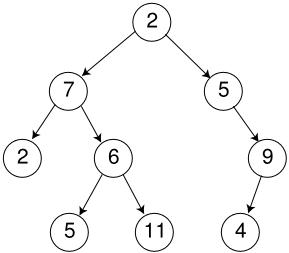
\includegraphics[width=4.671cm,height=4.129cm]{image/a2012Logique2eme-img033.jpg} 
		\end{center}
		
		Attention, l'arbre binaire n'est pas un cas particulier d'arbre 
		\textit{n}-aire (avec la valeur 2 pour \textit{n}), car les deux fils 
		d'un n{\oe}ud sont liés à une orientation~(gauche ou droit). 
		Dans le cas où un n{\oe}ud ne possède qu'un fils, il faut clairement 
		indiquer dans le schéma d'un arbre binaire s'il s'agit du fils 
		gauche ou droite, on ne peut donc jamais représenter un fils 
		à la verticale du père.

		Ainsi, dans l'exemple ci-dessus, le n{\oe}ud 9 est le fils 
		droit du n{\oe}ud 5, et le n{\oe}ud 4 est le fils gauche du
		n{\oe}ud 9.

	\subsection{Implémentation}
	%==========================
		
		Elle se déduit de l'implémentation de l'arbre «~quelconque~». 
		Pour le n{\oe}ud d'arbre binaire, la liste des fils est
		remplacée par deux liens~: un vers le fils gauche et un autre 
		vers le fils droit.

		\cadre{
			\begin{pseudo}
				\Class{N{\oe}udBinaire<T>}
					\Private 
						\Decl valeur~: T
						\Decl gauche~: <{N{\oe}udBinaire<T>}>
						\Decl droit~: <{N{\oe}udBinaire<T>}>
					\Public 
						\ConstrSign{N{\oe}udBinaire<T>}{val~: T}
						\RComment construit un n{\oe}ud sans fils
						\MethodSign{getValeur}{}{T}
						\MethodSign{setValeur}{val~: T}{}
						\MethodSign{getGauche}{}{N{\oe}udBinaire<T>}
						\MethodSign{setGauche}{fils~: N{\oe}udBinaire<T>}{}
						\MethodSign{getDroit}{}{N{\oe}udBinaire<T>}
						\MethodSign{setDroit}{fils~: N{\oe}udBinaire<T>}{}
				\EndClass
			\end{pseudo}
		}
		
		\cadre{
			\begin{pseudo}
				\Class{ArbreBinaire<T>}
					\Private
						\Decl racine~: N{\oe}udBinaire<T>
					\Public 
						\ConstrSign{ArbreBinaire<T>}{}
						\RComment construit un arbre vide
						\MethodSign{getRacine}{}{N{\oe}udBinaire<T>}
						\MethodSign{setRacine}{r~: N{\oe}udBinaire<T>}{}
				\EndClass
			\end{pseudo}
		}


%====================================
\section{Parcours de l'arbre binaire}
%====================================

	\subsection{Parcours en largeur}
	%===============================

		La boucle «~pour~» du parcours de l'arbre «~quelconque~» 
		est remplacée ici par la mise en file de chacun des fils du
		n{\oe}ud courant. Il faut toutefois prendre garde de ne 
		pas mettre de lien vide dans la file.
		
		\cadre{
			\begin{pseudo}
				\Module{parcoursLargeur}{monArbre~: ArbreBinaire<T>}{}
					\Decl maFile~: File<{N{\oe}udBinaire<T>}>
					\Decl n{\oe}udCourant~: N{\oe}udBinaire<T>
					\Decl i~: entier
					\Let maFile \Gets \K{nouveau} File<{N{\oe}udBinaire<T>}>
					\If{monArbre.getRacine( ) ${\neq}$ rien}
						\Stmt maFile.enfiler(monArbre.getRacine( ))
					\EndIf
					\While{NON maFile.estVide( )}
						\Let n{\oe}udCourant \Gets maFile.défiler( )
						\LComment traitement du n{\oe}ud courant
						\If{n{\oe}udCourant.getGauche( ) ${\neq}$ rien}
							\Stmt maFile.enfiler(n{\oe}udCourant.getGauche( ))
						\EndIf
						\If{n{\oe}udCourant.getDroit( ) ${\neq}$ rien}
							\Stmt maFile.enfiler(n{\oe}udCourant.getDroit( ))
						\EndIf
					\EndWhile
				\EndModule
			\end{pseudo}
		}
	
	\subsection{Parcours en profondeur}
	%==================================
	
		Pour les arbres binaires, aux parcours en profondeur préfixé 
		et postfixé s'ajoute le \textbf{parcours infixé}~: le
		traitement d'un n{\oe}ud se fait entre les parcours de son 
		sous-arbre gauche et de son sous-arbre droit.
		
		\cadre{
			\begin{pseudo}
				\Module{parcoursProfondeur}{monArbre~: ArbreBinaire<T>}{}
					\Stmt parcoursProfondeurRécursif(monArbre.getRacine( ))
				\EndModule
			\end{pseudo}
		}
		
		\cadre{
			\begin{pseudo}
				\Module{parcoursProfondeurRécursif}{n{\oe}udCourant~: N{\oe}udBinaire<T>}{}
					\If{n{\oe}udCourant ${\neq}$ rien}
						\LComment instructions de traitement du n{\oe}ud courant si parcours préfixé (ou RGD)
						\Stmt parcoursProfondeurRécursif(n{\oe}udCourant.getGauche( ))
						\LComment instructions de traitement du n{\oe}ud courant si parcours infixé (ou GRD)
						\Stmt parcoursProfondeurRécursif(n{\oe}udCourant.getDroit( ))
						\LComment instructions de traitement du n{\oe}ud courant si parcours postfixé (ou GDR)
					\EndIf
				\EndModule
			\end{pseudo}
		}
		
		{\itshape
		Par exemple, pour l'arbre binaire représenté ci-dessous~:}

		\begin{center}
		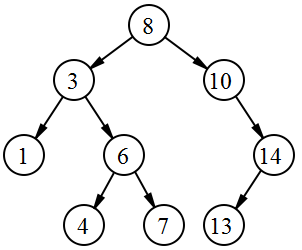
\includegraphics[width=4.457cm,height=3.687cm]{image/a2012Logique2eme-img034.png}
		\end{center}
		
		{\itshape
		les ordres de traitements sont les suivants~:
		
		\begin{itemize}
			\item {
				parcours en largeur~: 8, 3, 10, 1, 6, 14, 4, 7, 13}
			\item {
				parcours en profondeur préfixé~: 8, 3, 1, 6, 4, 7, 10, 14, 13}
			\item {
				parcours en profondeur infixé~: 1, 3, 4, 6, 7, 8, 10, 13, 14}
			\item {
				parcours en profondeur postfixé~: 1, 4, 7, 6, 3, 13, 14, 10, 8}
		\end{itemize}
		}
		
		
%==============================
\section{Arbre binaire ordonné}
%==============================

	\subsection{Définition}
	%======================

	Un arbre binaire est ordonné si pour tout n{\oe}ud, toutes les valeurs 
	de son sous-arbre gauche sont inférieures ou égales à la valeur 
	du n{\oe}ud, et toutes les valeurs de son sous-arbre droit sont 
	strictement supérieures à la valeur du n{\oe}ud.

	{\itshape Exemple~:}

	\begin{center}
	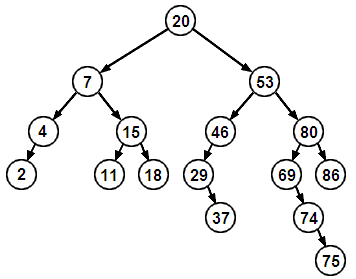
\includegraphics[width=6.994cm,height=5.486cm]{image/a2012Logique2eme-img035.png}
	\end{center}
	
	Cette structure se prête assez bien aux opérations de recherche, 
	d'ajout, de suppression car elle permet de localiser
	rapidement le n{\oe}ud où doit être exécuté l'opération, 
	tout en offrant une souplesse dans ses modifications (comme
	pour une liste chainée). La recherche s'apparente à la 
	recherche dichotomique dans un tableau, et si l'arbre est
	\textit{équilibré} (pour une définition précise de ce terme, 
	voir énoncé de l'ex. 9), toutes les opérations citées ont
	une complexité en O($log_2^n$).

	Pour obtenir la liste des valeurs d'un arbre binaire ordonné 
	dans l'ordre, il suffit de parcourir ses n{\oe}uds par le
	parcours en profondeur infixé.



%==================
\section{Exercices}
%==================

	\subsection{arbre quelconque ou binaire}
	%=======================================
		Les exercices 1 à 8 peuvent être résolus indifféremment 
		dans le cas d{}'un arbre quelconque ou d'un arbre binaire.

		\begin{Exercice}{Combien de n{\oe}uds~?}
			Écrire un algorithme qui compte le nombre total de 
			n{\oe}uds contenus dans un arbre.
		\end{Exercice}
		
		\begin{Exercice}{Et combien de feuilles~?}
			Écrire un algorithme qui compte le nombre de feuilles que possède un arbre.
		\end{Exercice}
		
		\begin{Exercice}{Hauteur}
			Écrire un algorithme qui calcule la hauteur d'un arbre, 
			c'est-à-dire la plus grande hauteur (ou la plus grande
			profondeur) de ses n{\oe}uds.
		\end{Exercice}
		
		\begin{Exercice}{Problème de niveau}
			Écrire un algorithme qui retourne le nombre de n{\oe}uds 
			d'un arbre situés à un niveau donné (valeur entière entrée en
			paramètre).
		\end{Exercice}

		\begin{Exercice}{Tout le monde est là~?}
			Écrire un algorithme qui vérifie si un arbre est complet.
		\end{Exercice}

		\begin{Exercice}{Arbre dégénéré}
			Écrire un algorithme qui indique si un arbre est dégénéré ou non.
		\end{Exercice}
		
		\begin{Exercice}{Additions}
			Soit un arbre d'entiers dont seules les feuilles ont été 
			affectées par des valeurs. Compléter l'arbre de telle sorte que
			la valeur de chaque n{\oe}ud soit égale à la somme des valeurs de ses fils.

			\begin{flushleft}
			\tablefirsthead{}
			\tablehead{}
			\tabletail{}
			\tablelasttail{}
			\begin{supertabular}{m{5.215cm}m{5.217cm}m{5.217cm}}
			 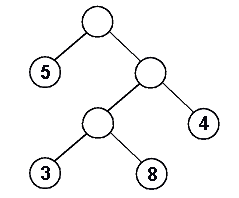
\includegraphics[width=4.406cm,height=3.667cm]{image/a2012Logique2eme-img036.png}  &
			~

			~

			~

			{ devient après remplissage [F0E0?]} &
			 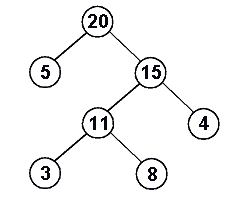
\includegraphics[width=4.773cm,height=3.955cm]{image/a2012Logique2eme-img037.png} \\
			\end{supertabular}
			\end{flushleft}

		\end{Exercice}
		
		\begin{Exercice}{Combien de valeurs~?}
			Écrire un algorithme qui indique le nombre de valeurs différentes 
			que contient un arbre.
		\end{Exercice}
		
	\subsection{Arbres binaires}
	%===========================

		\begin{Exercice}{Arbre binaire équilibré}
			Dans un arbre binaire, on définit le \textbf{facteur d'équilibre} 
			d'un n{\oe}ud de la façon suivante~: c'est la différence entre 
			la hauteur de son sous-arbre gauche et celle de son sous-arbre droit. 
			On dit que l'arbre est \textbf{équilibré} si, pour tout n{\oe}ud 
			de l'arbre, ce facteur d'équilibre est compris entre --1 et 1.
		\end{Exercice}
		
		\begin{Exercice}{Arbre binaire pair}
			Un arbre binaire est \textbf{pair} si chacun de ses n{\oe}uds 
			a soit 2 fils, soit aucun. Écrire un algorithme qui
			vérifie si un arbre binaire possède cette propriété. 
			
			N. B.~: un arbre vide est pair.
		\end{Exercice}
		
		\begin{Exercice}{OXO}
			Soit un arbre binaire de caractères. Vérifier s'il contient 
			la configuration 'O'-'X'-'O' formée respectivement par un
			fils gauche, un père et un fils droit.
		\end{Exercice}

		\begin{Exercice}{Arbre binaire symétrique}
			Écrire un algorithme qui vérifie si un arbre binaire est 
			\textbf{symétrique}, c'est-à-dire si le sous-arbre gauche de la
			racine est identique en miroir à son sous-arbre droit.

			\begin{center}
			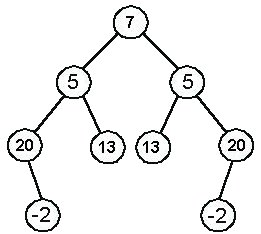
\includegraphics[width=4.805cm,height=4.307cm]{image/a2012Logique2eme-img038.jpg}
			\end{center}
		\end{Exercice}
		
	\subsection{Arbres binaires ordonnés}
	%====================================

		\begin{Exercice}{L'arbre binaire est-il ordonné~?}
			Écrire un algorithme qui vérifie si un arbre binaire est ordonné.
		\end{Exercice}
		
		\begin{Exercice}{Le maximum}
			Écrire un algorithme qui retourne la valeur maximum d'un arbre 
			binaire ordonné.
		\end{Exercice}
		
		\begin{Exercice}{Recherche dichotomique}
			Écrire un algorithme qui recherche dans un arbre binaire la 
			présence d'un n{\oe}ud de valeur donnée, et en retourne
			l'accès. Si la valeur ne se trouve pas dans l'arbre, 
			l'algorithme retourne \textit{rien} dans ce cas.
		\end{Exercice}
		
		\begin{Exercice}{Ajout de valeur}
			Écrire un algorithme qui ajoute un n{\oe}ud dans un arbre 
			binaire ordonné, dont la valeur est entrée en paramètre.
		\end{Exercice}
		
	\subsection{Arbres quelconques}
	%==============================
			
			\begin{Exercice}{Le dictionnaire}
				Utilisons un arbre pour stocker les mots d'un dictionnaire. 
				Les lettres d'un mot sont représentées chacune par
				un n{\oe}ud à un niveau différent et les mots ayant 
				le même début partagent leurs n{\oe}uds. De plus, un caractère
				spécial indique la fin d'un mot. La racine ne contient 
				rien. Les fils d'un n{\oe}ud ne sont pas forcément dans 
				l'ordre	alphabétique.
				
				Dans l'exemple ci-dessous, le dictionnaire contient les mots 
				AI,~AIL, AIT, AS, SA, SOL, SOT, Y.
				\begin{center}
				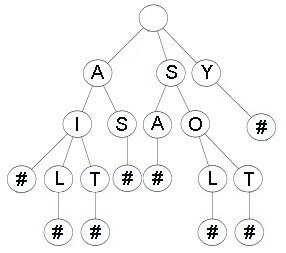
\includegraphics[width=6.999cm,height=6.195cm]{image/a2012Logique2eme-img039.jpg}
				\end{center}
				
				Écrire un algorithme~:
				
				\begin{enumerate}
					\item {
						qui affiche tous les mots du dictionnaire}
					\item {
						qui ajoute un mot dans le dictionnaire}
					\item {
						qui enlève un mot du dictionnaire}
				\end{enumerate}
			\end{Exercice}
			
			\begin{Exercice}{Au fil de l'eau}
				Les cours d'eau d'un bassin fluvial peuvent être schématisés 
				avec un arbre~: la racine contient le nom du fleuve, 
				et les fils d'un n{\oe}ud sont les affluents du fleuve 
				ou des rivières faisant partie du bassin fluvial.
				\begin{center}
				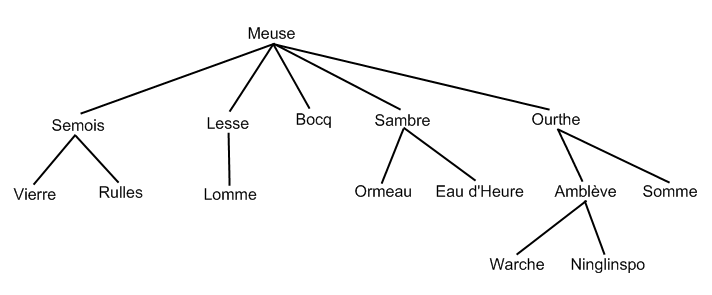
\includegraphics[width=11.529cm,height=4.768cm]{image/a2012Logique2eme-img040.png}
				\end{center}
				Écrire un algorithme qui reçoit le nom d'un cours d'eau 
				en paramètre et affiche la suite des rivières qui
				le conduisent au fleuve principal. Par exemple, 
				pour \textit{«~Somme~»}, l'algorithme affiche \textit{«~Somme~»}, 
				\textit{«~Ourthe~»} et \textit{«~Meuse~»}.
			\end{Exercice}
								
%%====================
\chapter{Les graphes}
%====================

\begin{center}
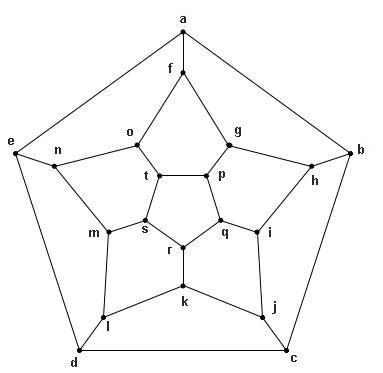
\includegraphics[width=4.092cm,height=3.999cm]{image/a2012Logique2eme-img041.jpg}
\end{center}
	

%================
\section{Utilité}
%================

	La théorie des graphes permet de répondre à différents 
	problèmes se formulant en termes d'\textbf{objets} et de
	\textbf{liens} entre ceux-ci. De nombreux problèmes relatifs 
	à l'étude des réseaux peuvent être résolus grâce à la
	théorie des graphes, que ce soit des problèmes de voyage 
	(réseaux aériens, routiers, ferroviaires) ou des problèmes de
	communication entre personnes (réseaux téléphoniques) 
	ou entre ordinateurs (réseaux informatiques, internet, ...)

	Un problème classique de la théorie des graphes, et qui a 
	prouvé toute son utilité depuis l'invention du GPS, est la
	détermination du chemin le plus rapide (ou le plus court 
	ou encore le moins coûteux) entre deux localisations
	géographiques. Pour résoudre ce type de problème, il faut 
	connaitre les différents relais ou points de passage (objets)
	et savoir lesquels sont reliés entre eux par des routes 
	(les liens), ainsi que des informations supplémentaires sur ces
	liens (distance, type de route, etc.).

	Un autre pilier de la théorie des graphes est l'étude de 
	l'ordonnancement des tâches. Quelles sont les contraintes
	conditionnant l'avancement d'un projet ? Quelle tâche doit 
	être finie avant que telle autre ne commence ? Comment tenir
	compte des tâches concurrentes ?

	D'autres domaines peuvent également être abordés~:

	\begin{itemize}
		\item {
			analyse d'un programme, d'un algorithme}
		\item {
			élaboration de cartes géographiques}
		\item {
			représentation de relations entre individus (familiales, professionnelles, ...)}
		\item {
			représentation d'automates d'états finis, de tables de décisions, ...}
	\end{itemize}
	
	Le but de cette partie du cours n'est pas d'aborder jusque 
	dans les moindres détails la théorie des graphes. Celle-ci et
	ses développements sont d'une telle richesse qu'ils font 
	l'objet de nombreux ouvrages spécialisés. Nous nous limiterons
	à un aperçu synthétisé permettant de situer les problèmes et de 
	servir de tremplin à une étude personnelle plus approfondie.

%=====================
\section{Terminologie}
%=====================

	N.B.~Les graphes vous sont déjà familiers, puisqu'ils 
	ont déjà été étudiés au cours de mathématique de
	1\textsuperscript{ère} année. Nous rappelons brièvement 
	ici les principales définitions, et renvoyons le lecteur au
	syllabus de mathématique de 1\textsuperscript{ère} 
	pour plus de précision.

	\subsection{Définition}
	%======================

		Un \textbf{graphe} est un modèle mathématique représentant 
		les liens existant entre différents objets de même type,
		appelés \textbf{n{\oe}uds} ou \textbf{sommets}. Les liens 
		sont appelés \textbf{arcs} ou \textbf{arêtes}, selon que le
		graphe est orienté ou non. On peut donc voir un graphe comme 
		l'association de l'ensemble $S$ de ses n{\oe}uds et de
		l'ensemble $A$ de ses arêtes~:

		\begin{center}
			$G = (S, A)$
		\end{center}


		On représente schématiquement un graphe par un ensemble de 
		points reliés entre eux par des traits ou des lignes
		représentant ces liens.

	\subsection{Types de graphes}
	%=============================
	
		\subsubsection{Graphe orienté}
		%=============================
		
			Un graphe est \textbf{orienté} lorsque ses n{\oe}uds 
			sont reliés par des \textbf{arcs}. Un arc est un \textbf{couple}
			$(u, v)$ de n{\oe}uds, où $u$ est l'\textbf{origine} du couple 
			(ou encore le \textit{prédécesseur}, le	\textit{départ} ou 
			l'\textit{extrémité initiale}) et $v$ l'\textbf{extrémité} 
			(ou encore le \textit{successeur}, l'\textit{arrivée} ou 
			l'\textit{extrémité terminale}). On dira de cet arc qu'il 
			\textit{part} du n{\oe}ud $u$ et qu'il \textit{arrive} au 
			n{\oe}ud $v$. Dans la représentation schématique d'un graphe 
			orienté, on représente habituellement les arcs par des flèches 
			qui traduisent le sens de la relation entre deux n{\oe}uds.

			\textbf{Exemple~:} G = (S, A) avec S = \{A, B, C, D, E\} et 
			A = \{(A, D), (A, E), (B, A), (B, E), (C, A), (C, E), (D, B), (D, C),
			(E, D)\}

			\begin{center}
			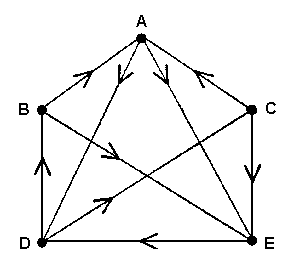
\includegraphics[width=5.159cm,height=4.598cm]{image/a2012Logique2eme-img042.png}
			\end{center}
			
			Un graphe orienté peut aussi contenir des boucles~: 
			une \textbf{boucle} est un arc dont l'origine et l'extrémité sont
			identiques, elle part et arrive au même n{\oe}ud.

			Un graphe orienté est dit \textbf{symétrique} si l'existence 
			d'un arc allant de $u$ vers $v$ implique l'existence d'un arc 
			«~réciproque~» de $v$ vers $u$ (avec $u \neq v$).
			

		\subsubsection{Graphe non orienté}
		%=================================
			
			Dans un graphe \textbf{non orienté}, les n{\oe}uds sont 
			reliés par des \textbf{arêtes}. Une arête est une \textbf{paire}
			$\{u, v\}$ de n{\oe}uds, c'est-à-dire un ensemble non ordonné 
			de deux n{\oe}uds (pour rappel,
			$\{u, v\}$ = $\{v, u\}$)

			\textbf{Exemple~:} G = (S, A) avec S = \{A, B, C, D, E, F\} et 
			A = \{\{A, B\}, \{A, E\}, \{B, C\}, \{C, D\}, \{C, F\}, \{D, E\},
			\{D, F\}, \{E, F\}\}

			\begin{center}
			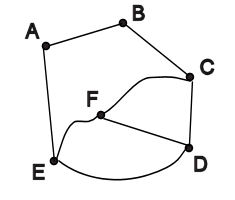
\includegraphics[width=4.284cm,height=3.657cm]{image/a2012Logique2eme-img043.jpg}
			\end{center}

			Remarquons qu'un graphe non orienté peut être représenté par un 
			graphe orienté~: il suffit de remplacer chaque arête
			reliant deux n{\oe}uds distincts par deux arcs orienté (ce qui donne 
			un graphe symétrique). L'inverse n'est évidemment pas vrai !

		\subsubsection{Multigraphe}
		%==========================
			
			Lorsqu'on admet que deux n{\oe}uds d'un graphe peuvent 
			être rejoints par plusieurs arcs ou arêtes, on parle de
			\textbf{multigraphe}. Ce type de graphe est par exemple 
			utilisé en chimie pour la représentation des molécules, un
			double lien représentant une liaison plus forte entre 
			les atomes d'une molécule.

			\begin{center}
			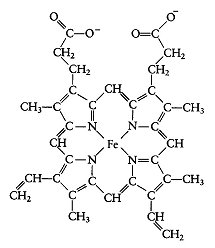
\includegraphics[width=5.172cm,height=5.974cm]{image/a2012Logique2eme-img044.jpg}
			\end{center}

		\subsubsection{Graphe pondéré}
		%=============================
			
			Lorsqu'on associe une valeur numérique à chaque arc ou 
			arête d'un graphe, on obtient un \textbf{graphe pondéré}.
			L'exemple le plus connu d'un tel graphe est la carte routière 
			sur laquelle on indique les distances le long des routes
			joignant deux points de repère. D'autres informations possibles 
			sont le temps, le coût, le poids, ...

			\begin{center}
			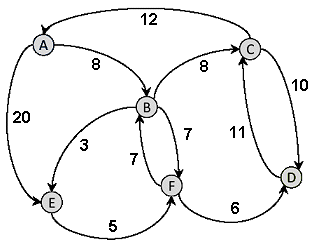
\includegraphics[width=9.038cm,height=7.091cm]{image/a2012Logique2eme-img045.png} 
			\end{center}
			
		\subsubsection{Graphe étiqueté}
		%==============================
		
			Un graphe est étiqueté lorsque ce sont des informations 
			de type texte qui sont attachées sur chaque arc ou arête (par
			exemple les numéros des routes sur une carte routière~: «~A19~» ou «~E40~», ...)


	\subsection{Adjacence, incidence et degré}
	%=========================================
		
		On dit que deux n{\oe}uds sont \textbf{adjacents} 
		(ou \textbf{voisins}) s'il existe un arc (pour les graphes orientés)
		ou une arête (pour les graphes non orientés) reliant ces n{\oe}uds. 
		L'adjacence s'applique aussi aux liens~: deux arcs (ou deux arêtes) 
		sont \textbf{adjacents} lorsqu'ils ont un n{\oe}ud en commun. 
		Par contre, la relation entre les n{\oe}uds et les liens s'exprime 
		en terme d'\textbf{incidence}~: on dit qu'un arc ou une arête est 
		\textbf{incident} à un n{\oe}ud.

		Un graphe non orienté dans lequel chaque n{\oe}ud est adjacent 
		à tous les autres n{\oe}uds est dit \textbf{complet}.
		Pour un graphe orienté, un graphe complet est tel qu'en 
		chaque n{\oe}ud partent des arcs vers tous les autres n{\oe}uds.

		Le degré d'un n{\oe}ud est le nombre d'arcs (ou d'arêtes) 
		incidents à ce n{\oe}ud. Dans le cas d'un graphe orienté, 
		on définit encore~:
		
		\begin{itemize}
			\item {
				le \textbf{degré entrant} d'un n{\oe}ud~: 
				c'est le nombre d'arcs qui arrivent en ce n{\oe}ud}
			\item {
				le \textbf{degré sortant} d'un n{\oe}ud~: 
				c'est le nombre d'arcs qui partent de ce n{\oe}ud}
		\end{itemize}
		
		Toujours dans le cas des graphes orientés, un \textbf{puits} 
		est un n{\oe}ud dont le degré sortant est nul~: arrivé dans
		un puits, on ne peut plus en sortir ! Inversement, une 
		\textbf{source} est un n{\oe}ud dont le degré entrant est nul.
		On peut donc partir d'une source, mais on ne peut plus 
		jamais y revenir ! Si les degrés entrant et sortant sont tous
		les deux nuls, on a alors un n{\oe}ud isolé.

		\textbf{Exemple~:} dans le graphe ci-dessous, 
		le n{\oe}ud 8 est de degré 3 ; son degré entrant est 2 
		et son degré sortant est 1.
		Les n{\oe}uds 1, 3 et 5 sont des sources, 
		et les n{\oe}uds 6 et 7 sont des puits.

		\begin{center}
		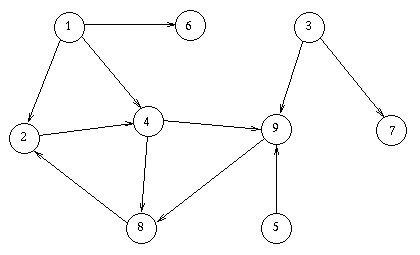
\includegraphics[width=7.527cm,height=4.56cm]{image/a2012Logique2eme-img046.jpg}
		\end{center}
		
		\textbf{Remarque~:} une boucle compte pour deux dans le calcul du degré 
		d'un n{\oe}ud, que ce soit dans un graphe orienté ou non orienté.
		
	\subsection{Chemin, cycle et connexité}
	%======================================
	
		\subsubsection{Chemin}
		%=====================
		
			Dans un graphe orienté, un \textbf{chemin} est une 
			suite d'arcs adjacents de la forme~:

			\begin{center}
			$(u_0, u_1)$, $(u_1, u_2)$, $(u_2, u_3)$, ..., $(u_{n-1}, u_n)$
			\end{center}

			Dans cette suite, chaque arc part du n{\oe}ud où arrive 
			l'arc précédent. Dans un graphe non orienté, la définition est
			analogue~: un chemin (aussi appelé \textbf{chaine} dans ce cas) 
			est une suite d'arêtes adjacentes. 

			Un chemin est \textbf{simple} si tous ses arcs (ou arêtes) sont distincts. 
			N.B.~: dans tout ce qui suit, nous ne considérerons uniquement 
			que les chemins simples.

			Un chemin est \textbf{élémentaire} si tous ses n{\oe}uds 
			(sauf éventuellement le premier et le dernier) sont distincts.


			La \textbf{longueur} d'un chemin est le nombre d'arcs (ou d'arêtes) 
			qui composent ce chemin. La \textbf{distance} entre deux n{\oe}uds 
			est le minimum des longueurs parmi tous les chemins qui relient 
			ces deux n{\oe}uds. Enfin, le \textbf{diamètre} d'un graphe est la 
			plus grande distance possible entre deux n{\oe}uds quelconques 
			de ce graphe.

			N.B.~: on pourrait aussi décrire un chemin en donnant une suite de 
			n{\oe}uds adjacents plutôt qu'une suite d'arcs ou d'arêtes.

			\textbf{Exemple~:} 
			La suite d'arêtes \{2, 3\}, \{3, 4\}, \{4, 5\}, \{5, 6\}, \{6, 7\} 
			du graphe non orienté ci-dessous forme un chemin de longueur 5. 
			La distance entre les n{\oe}uds 2 et 7 est toutefois 3, 
			car la longueur du chemin \{2, 3\}, \{3, 4\}, \{4, 7\} est plus courte. 
			Le diamètre de ce graphe est 5.

			\begin{center}
			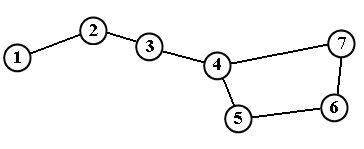
\includegraphics[width=8.641cm,height=3.542cm]{image/a2012Logique2eme-img047.jpg}
			\end{center}
			
		\subsubsection{Circuits et cycles}
		%=================================
			
			Dans un graphe orienté, un \textbf{circuit} est un chemin fermé, 
			c'est-à-dire une suite d'au minimum 2 arcs dont le n{\oe}ud de 
			départ est identique au n{\oe}ud d'arrivée. Pour un graphe non 
			orienté, on parle plutôt de \textbf{cycle}~:
			c'est également un chemin fermé constitué d'au moins 3 arêtes 
			adjacentes. Un circuit (ou un cycle) est \textbf{simple}
			ou \textbf{élémentaire} selon que le chemin correspondant 
			peut être qualifié de la même façon.

			Dans l'exemple ci-dessus, la suite d'arêtes 
			\{4, 5\}, \{5, 6\}, \{6, 7\}, \{7, 4\} 
			forme un cycle élémentaire de	longueur 4.

		\subsubsection{Connexité}
		%========================
		
		Un graphe \textbf{non orienté} est \textbf{connexe} 
		(ou \textbf{connecté}) s'il existe toujours un chemin 
		reliant deux n{\oe}uds quelconques de ce graphe. 
		Autrement dit, un graphe connexe est «~d'un seul tenant~».

		Une \textbf{composante connexe} d'un graphe est un sous-ensemble 
		de n{\oe}uds et d'arêtes de ce graphe formant lui-même
		un graphe connexe, et tel qu'il n'existe aucun chemin reliant 
		un de ses n{\oe}uds à un n{\oe}ud hors de ce sous-ensemble.

		Pour un graphe \textbf{orienté}, la définition de connexité est 
		analogue, toutefois en considérant les arcs sans leur orientation.

		Un graphe connexe ne possédant aucun cycle est un \textbf{arbre}, 
		et un graphe dont toutes les composantes connexes sont des arbres 
		est une \textbf{forêt}. Attention, ne pas confondre cette 
		définition d'arbre avec les arbres binaires et \textit{n}-aires 
		étudiés précédemment. Dans le contexte d'un graphe, il n'y a pas 
		de notion de racine, de niveau, de hauteur, de n{\oe}uds père et fils, etc. 
		Par contre, les n{\oe}uds d'un arbre qui sont de degré 1 portent aussi le
		nom de \textbf{feuilles}.

		\textbf{Exemple~:} Dans le graphe suivant, il y a trois composantes 
		connexes, respectivement formées par les sous-ensembles de n{\oe}uds 
		\{1, 2, 3, 4, 5, 6, 7, 8, 9\}, \{10, 11, 12\} et \{13, 14, 15\}. 
		La 3\textsuperscript{ème} de ces composantes est un arbre.

		\begin{center}
		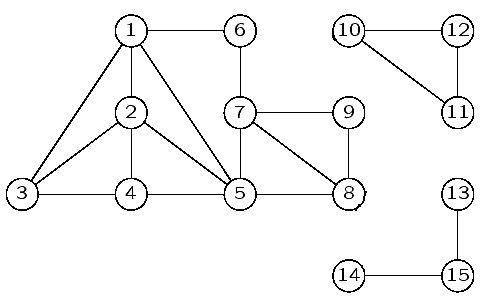
\includegraphics[width=6.235cm,height=3.955cm]{image/a2012Logique2eme-img048.jpg}
		\end{center}



%==================================
\section{Implémentation en mémoire}
%==================================

	\subsection{Représentation des n{\oe}uds}
	%========================================
				
		Dans les exemples précédents, les n{\oe}uds des graphes étaient 
		nommés par des lettres ou des numéros, mais ils peuvent
		contenir de l'information diverse. Par ex. dans le graphe 
		d'un réseau de métro, les n{\oe}uds seraient des chaines
		(noms des stations) ; en théorie des jeux, les n{\oe}uds 
		peuvent contenir la configuration complète de l'état d'un jeu,
		les arêtes représentant alors les possibilités de passage 
		d'une configuration à une autre. Le type des n{\oe}uds
		détermine le type du graphe~: on parlera d'un graphe d'entiers, 
		de chaines,... et de façon générique, d'un graphe de type T.

		Le contenu des n{\oe}uds peut être stocké dans un tableau ou une 
		liste, selon le contexte. Un tableau convient bien pour
		implémenter un problème de graphe «~statique~» (où le nombre 
		de n{\oe}uds reste fixe) et la liste pour la modélisation
		d'un graphe qui subirait des transformations (ajout ou 
		suppression de n{\oe}uds). Dans tous les cas, on considère qu'il
		est toujours possible de numéroter les n{\oe}uds de 1 à \textit{n}.

	\subsection{Représentation des arcs/arêtes}
	%==========================================
				
		\subsubsection{Représentation matricielle}
		%=========================================

			La représentation matricielle est la façon la plus évidente 
			pour représenter les arêtes d'un graphe. Si seule
			l'existence des liens doit être représentée, on utilise une 
			matrice de booléens appelée \textbf{matrice d'adjacence}
			(ou \textbf{matrice de contigüité}). Chaque ligne et chaque 
			colonne de cette matrice correspond à un n{\oe}ud du
			graphe, conformément à la numérotation des n{\oe}uds choisie.

			Pour un graphe orienté, les lignes correspondent à l'origine des 
			arcs et les colonnes à leur extrémité. Ainsi, l'élément
			d'indices $(i, j)$ sera \textbf{vrai} si un arc 
			part de $i$ et arrive en $j$.

			\textbf{Exemple~:} Le graphe orienté ci-dessous à gauche 
			peut être représenté par la matrice d'adjacence à droite.

			\begin{center}
				\tablefirsthead{}
				\tablehead{}
				\tabletail{}
				\tablelasttail{}
				\begin{supertabular}{m{7.0350003cm}m{0.81600004cm}m{0.81600004cm}|m{0.81600004cm}|m{0.81600004cm}|m{0.81600004cm}|m{0.81600004cm}|m{0.81600004cm}|}
				\centering  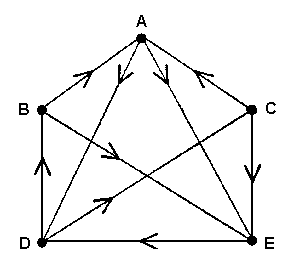
\includegraphics[width=4.318cm,height=3.859cm]{image/a2012Logique2eme-img049.png}  &
				~
				 &
				\multicolumn{1}{m{0.81600004cm}}{~
				} &
				\multicolumn{1}{m{0.81600004cm}}{\centering{ A}} &
				\multicolumn{1}{m{0.81600004cm}}{\centering{ B}} &
				\multicolumn{1}{m{0.81600004cm}}{\centering{ C}} &
				\multicolumn{1}{m{0.81600004cm}}{\centering{ D}} &
				\multicolumn{1}{m{0.81600004cm}}{\centering\arraybslash{ E}}\\\hhline{~~~-----}
				 &
				~
				 &
				\centering{ A} &
				\centering{ F} &
				\centering{ F} &
				\centering{ F} &
				\centering{ V} &
				\centering\arraybslash{ V}\\\hhline{~~~-----}
				 &
				~
				 &
				\centering{ B} &
				\centering{ V} &
				\centering{ F} &
				\centering{ F} &
				\centering{ F} &
				\centering\arraybslash{ V}\\\hhline{~~~-----}
				 &
				~
				 &
				\centering{ C} &
				\centering{ V} &
				\centering{ F} &
				\centering{ F} &
				\centering{ F} &
				\centering\arraybslash{ V}\\\hhline{~~~-----}
				 &
				~
				 &
				\centering{ D} &
				\centering{ F} &
				\centering{ V} &
				\centering{ V} &
				\centering{ F} &
				\centering\arraybslash{ F}\\\hhline{~~~-----}
				 &
				~
				 &
				\centering{ E} &
				\centering{ F} &
				\centering{ F} &
				\centering{ F} &
				\centering{ V} &
				\centering\arraybslash{ F}\\\hhline{~~~-----}
				 &
				~
				 &
				\multicolumn{1}{m{0.81600004cm}}{~
				} &
				\multicolumn{1}{m{0.81600004cm}}{~
				} &
				\multicolumn{1}{m{0.81600004cm}}{~
				} &
				\multicolumn{1}{m{0.81600004cm}}{~
				} &
				\multicolumn{1}{m{0.81600004cm}}{~
				} &
				\multicolumn{1}{m{0.81600004cm}}{~
				}\\
				\end{supertabular}
			\end{center}
			
			Dans le cas d'un graphe non orienté, l'élément d'indices $(i, j)$ 
			est mis à \textbf{vrai} si une arête rejoint les n{\oe}uds $i$ et $j$. 
			Comme cette relation est symétrique, la matrice d'adjacence qui en
			résulte est une \textbf{matrice symétrique}, c'est-à-dire que 
			$m_{ij} = m_{ji} \forall{i, j}$. Par économie, on peut aussi se limiter 
			dans ce cas à une \textbf{matrice triangulaire}, où seule une moitié 
			de la matrice est utilisée (par exemple les éléments $m{ij}$ 
			tels que $j \geq i$ s'il y a des boucles et $j > i$ sinon).

			\textbf{Exemple~:} Le graphe non orienté de la figure ci-dessous 
			peut être représenté par une matrice symétrique (à gauche) ou
			triangulaire supérieure (à droite).

			\begin{center}
			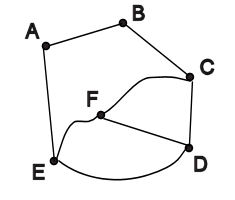
\includegraphics[width=3.784cm,height=3.233cm]{image/a2012Logique2eme-img050.jpg}
			\end{center}

			\begin{center}
				\tablefirsthead{}
				\tablehead{}
				\tabletail{}
				\tablelasttail{}
				\begin{supertabular}{m{0.93900007cm}|m{0.81600004cm}|m{0.81600004cm}|m{0.81600004cm}|m{0.81600004cm}|m{0.81600004cm}|m{0.81600004cm}|m{0.81600004cm}m{0.81600004cm}|m{0.81600004cm}|m{0.81600004cm}|m{0.81600004cm}|m{0.81600004cm}|m{0.81600004cm}|m{0.81600004cm}|}
				\multicolumn{1}{m{0.93900007cm}}{~
				} &
				\multicolumn{1}{m{0.81600004cm}}{\centering{ A}} &
				\multicolumn{1}{m{0.81600004cm}}{\centering{ B}} &
				\multicolumn{1}{m{0.81600004cm}}{\centering{ C}} &
				\multicolumn{1}{m{0.81600004cm}}{\centering{ D}} &
				\multicolumn{1}{m{0.81600004cm}}{\centering{ E}} &
				\multicolumn{1}{m{0.81600004cm}}{\centering{ F}} &
				~
				 &
				\multicolumn{1}{m{0.81600004cm}}{~
				} &
				\multicolumn{1}{m{0.81600004cm}}{\centering{ A}} &
				\multicolumn{1}{m{0.81600004cm}}{\centering{ B}} &
				\multicolumn{1}{m{0.81600004cm}}{\centering{ C}} &
				\multicolumn{1}{m{0.81600004cm}}{\centering{ D}} &
				\multicolumn{1}{m{0.81600004cm}}{\centering{ E}} &
				\multicolumn{1}{m{0.81600004cm}}{\centering\arraybslash{ F}}\\\hhline{~------~~------}
				\centering{ A} &
				\centering{ F} &
				\centering{ V} &
				\centering{ F} &
				\centering{ F} &
				\centering{ V} &
				\centering{ F} &
				~
				 &
				\centering{ A} &
				\centering{ F} &
				\centering{ V} &
				\centering{ F} &
				\centering{ F} &
				\centering{ V} &
				\centering\arraybslash{ F}\\\hhline{~------~~------}
				\centering{ B} &
				\centering{ V} &
				\centering{ F} &
				\centering{ V} &
				\centering{ F} &
				\centering{ F} &
				\centering{ F} &
				~
				 &
				\centering{ B} &
				\centering{ F} &
				\centering{ F} &
				\centering{ V} &
				\centering{ F} &
				\centering{ F} &
				\centering\arraybslash{ F}\\\hhline{~------~~------}
				\centering{ C} &
				\centering{ F} &
				\centering{ V} &
				\centering{ F} &
				\centering{ V} &
				\centering{ F} &
				\centering{ V} &
				~
				 &
				\centering{ C} &
				\centering{ F} &
				\centering{ F} &
				\centering{ F} &
				\centering{ V} &
				\centering{ F} &
				\centering\arraybslash{ V}\\\hhline{~------~~------}
				\centering{ D} &
				\centering{ F} &
				\centering{ F} &
				\centering{ V} &
				\centering{ F} &
				\centering{ V} &
				\centering{ V} &
				~
				 &
				\centering{ D} &
				\centering{ F} &
				\centering{ F} &
				\centering{ F} &
				\centering{ F} &
				\centering{ V} &
				\centering\arraybslash{ V}\\\hhline{~------~~------}
				\centering{ E} &
				\centering{ V} &
				\centering{ F} &
				\centering{ F} &
				\centering{ V} &
				\centering{ F} &
				\centering{ V} &
				~
				 &
				\centering{ E} &
				\centering{ F} &
				\centering{ F} &
				\centering{ F} &
				\centering{ F} &
				\centering{ F} &
				\centering\arraybslash{ V}\\\hhline{~------~~------}
				\centering{ F} &
				\centering{ F} &
				\centering{ F} &
				\centering{ V} &
				\centering{ V} &
				\centering{ V} &
				\centering{ F} &
				~
				 &
				\centering{ F} &
				\centering{ F} &
				\centering{ F} &
				\centering{ F} &
				\centering{ F} &
				\centering{ F} &
				\centering\arraybslash{ F}\\\hhline{~------~~------}
				\end{supertabular}
			\end{center}

			La représentation matricielle peut s'étendre aux cas des graphes 
			pondérés (en utilisant une matrice d'entiers contenant
			les poids des arêtes) ou d'un graphe étiqueté (matrice de chaines). 
			L'absence d'arc entre deux n{\oe}uds peut alors
			être signalée par des valeurs aberrantes (par exemple --1 
			ou «~infini~» pour des distances, «~rien~» pour le graphe
			étiqueté, ...).

			N.B.~: Quelle que soit la configuration choisie, la représentation 
			matricielle est cependant coûteuse en mémoire, car
			beaucoup d'éléments restent en général inoccupés. La matrice creuse 
			(voir ex. dans le chapitre sur les listes chainées)
			est plus appropriée à ce type de contenu.

		\subsubsection{Représentation par un tableau de listes}
		%======================================================
			
			L'idée est de faire correspondre à chaque n{\oe}ud la liste 
			des n{\oe}uds qui lui sont adjacents (pour un graphe
			orienté, ce sera la liste des n{\oe}uds pour lesquels un 
			arc part du n{\oe}ud considéré). Ces listes (qui peuvent
			éventuellement être chainées) sont contenues dans un tableau, 
			le \textbf{tableau des listes d'adjacence}, dont les
			indices correspondent à la numérotation des n{\oe}uds. 
			Les variantes de ce type de représentation sont nombreuses.

			L'avantage principal de cette représentation est le gain de 
			place en mémoire. Le désavantage est la perte de l'accès
			direct à l'information~: dans la matrice, on voit directement 
			si $i$ et $j$ sont adjacents, dans le cas du tableau, il faut 
			faire une recherche pour voir si $j$ se trouve dans la liste 
			d'indice $i$.

			\textbf{Exemple~:} voici une représentation du graphe orienté 
			de la page précédente sous forme de tableau de listes.
			\begin{center}
			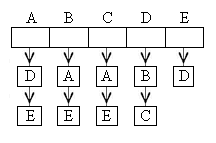
\includegraphics[width=5.715cm,height=3.784cm]{image/a2012Logique2eme-img051.png}
			\end{center}
			

%=========================
\section{Problèmes divers}
%=========================

	\subsection{Accessibilité d'un n{\oe}ud à partir d'un autre}
	%===========================================================

		Un n{\oe}ud $j$ est \textbf{accessible} à partir d'un n{\oe}ud $i$ 
		s'il existe un chemin partant de $i$ et arrivant à $j$. L'accessibilité 
		peut donc exister pour deux n{\oe}uds non adjacents. 
		Dans un graphe non orienté, l'accessibilité est assez évidente à établir~: 
		tous les n{\oe}uds d'une composante connexe du graphe sont forcément 
		accessibles. Le problème est moins immédiat et plus intéressant pour 
		les graphes orientés, et nous ne considérerons que ceux-ci 
		dans cette section.

		\subsubsection{Matrice d'accessibilité}
		%======================================

			Similairement à la matrice d'adjacence (qui indique si un n{\oe}ud 
			$i$ est en contact direct avec un n{\oe}ud $j$), la \textbf{matrice 
			d'accessibilité} est une matrice booléenne qui indique si à partir d'un 
			n{\oe}ud $i$, il existe un chemin qui mène au n{\oe}ud $j$. Comme 
			précédemment, l'indice ligne $i$ est associé à l'origine et l'indice 
			colonne $j$ à l'arrivée du chemin.

			\textbf{Exemple~:} Voici un graphe et sa matrice d'accessibilité. 
			On voit facilement que tous les n{\oe}uds sont accessibles à
			partir des n{\oe}uds 1 et 2. Par contre, les n{\oe}uds 3, 4 et 5 
			forment un cycle de longueur 3 duquel il n'est plus
			possible de retourner en 1 ou en 2.

			\begin{center}
				\tablefirsthead{}
				\tablehead{}
				\tabletail{}
				\tablelasttail{}
				\begin{supertabular}{m{7.0350003cm}m{0.81600004cm}m{0.81600004cm}m{0.81600004cm}|m{0.81600004cm}|m{0.81600004cm}|m{0.81600004cm}|m{0.81600004cm}|m{0.81600004cm}|}
				\centering  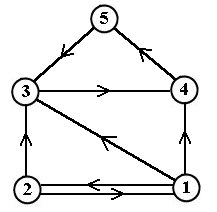
\includegraphics[width=4.355cm,height=4.247cm]{image/a2012Logique2eme-img052.jpg}  &
				~
				 &
				~
				 &
				\multicolumn{1}{m{0.81600004cm}}{~
				} &
				\multicolumn{1}{m{0.81600004cm}}{~
				} &
				\multicolumn{1}{m{0.81600004cm}}{~
				} &
				\multicolumn{1}{m{0.81600004cm}}{~
				} &
				\multicolumn{1}{m{0.81600004cm}}{~
				} &
				\multicolumn{1}{m{0.81600004cm}}{~
				}\\\hhline{~~~~-----}
				 &
				~
				 &
				~
				 &
				~
				 &
				\centering{ V} &
				\centering{ V} &
				\centering{ V} &
				\centering{ V} &
				\centering\arraybslash{ V}\\\hhline{~~~~-----}
				 &
				~
				 &
				~
				 &
				~
				 &
				\centering{ V} &
				\centering{ V} &
				\centering{ V} &
				\centering{ V} &
				\centering\arraybslash{ V}\\\hhline{~~~~-----}
				 &
				~
				 &
				~
				 &
				\centering{ \textit{A} =} &
				\centering{ F} &
				\centering{ F} &
				\centering{ V} &
				\centering{ V} &
				\centering\arraybslash{ V}\\\hhline{~~~~-----}
				 &
				~
				 &
				~
				 &
				~
				 &
				\centering{ F} &
				\centering{ F} &
				\centering{ V} &
				\centering{ V} &
				\centering\arraybslash{ V}\\\hhline{~~~~-----}
				 &
				~
				 &
				~
				 &
				~
				 &
				\centering{ F} &
				\centering{ F} &
				\centering{ V} &
				\centering{ V} &
				\centering\arraybslash{ V}\\\hhline{~~~~-----}
				 &
				~
				 &
				~
				 &
				\multicolumn{1}{m{0.81600004cm}}{~
				} &
				\multicolumn{1}{m{0.81600004cm}}{~
				} &
				\multicolumn{1}{m{0.81600004cm}}{~
				} &
				\multicolumn{1}{m{0.81600004cm}}{~
				} &
				\multicolumn{1}{m{0.81600004cm}}{~
				} &
				\multicolumn{1}{m{0.81600004cm}}{~
				}\\
				\end{supertabular}
			\end{center}
			
			Nous allons voir deux façons de générer la matrice d'accessibilité 
			en partant de la matrice d'adjacence d'un graphe.

		\subsubsection{Petit rappel de calcul matriciel}

			La somme de deux matrices de mêmes dimensions s'obtient en 
			additionnant les éléments de mêmes indices dans les deux
			matrices.
			
			Par exemple~:

			\begin{center}
				\tablefirsthead{}
				\tablehead{}
				\tabletail{}
				\tablelasttail{}
				\begin{supertabular}{|m{0.601cm}|m{0.601cm}|m{0.601cm}|m{0.601cm}m{0.601cm}m{0.601cm}|m{0.601cm}|m{0.601cm}|m{0.601cm}|m{0.601cm}m{0.601cm}m{0.601cm}|m{0.601cm}|m{0.601cm}|m{0.61800003cm}|}
				\hhline{---~~~---~~~---}
				\centering{ 1} &
				\centering{ 0} &
				\centering{ 4} &
				~
				 &
				~
				 &
				~
				 &
				\centering{ 3} &
				\centering{ 2} &
				\centering{ 1} &
				~
				 &
				~
				 &
				~
				 &
				\centering{ 4} &
				\centering{ 2} &
				\centering\arraybslash{ 5}\\\hhline{---~~~---~~~---}
				\centering{ {}--2} &
				\centering{ 2} &
				\centering{ 1} &
				~
				 &
				\centering{ +} &
				~
				 &
				\centering{ 2} &
				\centering{ 0} &
				\centering{ 3} &
				~
				 &
				\centering{ =} &
				~
				 &
				\centering{ 0} &
				\centering{ 2} &
				\centering\arraybslash{ 4}\\\hhline{---~~~---~~~---}
				\centering{ 3} &
				\centering{ 0} &
				\centering{ {}--1} &
				~
				 &
				~
				 &
				~
				 &
				\centering{ {}--2} &
				\centering{ 2} &
				\centering{ 0} &
				~
				 &
				~
				 &
				~
				 &
				\centering{ 1} &
				\centering{ 2} &
				\centering\arraybslash{ {}--1}\\\hhline{---~~~---~~~---}
				\end{supertabular}
			\end{center}

			La multiplication est un peu plus complexe~: 
			l'élément d'indices $(i, j)$ du produit de deux matrices
			est le \textit{produit scalaire} de la $i$\textsuperscript{ème} 
			ligne de la première matrice par la $j$\textsuperscript{ème} 
			colonne de la seconde. Le produit scalaire de deux vecteurs 
			(ou tableaux) de même taille est la somme des produits des 
			éléments de mêmes indices dans ces vecteurs. 
			
			En formule cela donne~:
			
			\begin{center}
			$(AB)_{ij} = \overset n{\underset{k=1}\sum} A_{ik} B_{kj}$
			\end{center}
			
			Attention, le produit matriciel n'est pas commutatif, 
			donc $AB \neq BA$ en général.

			\textbf{Exemple~:} pour obtenir l'élément d'indices (2, 1) 
			du produit, on calcule le produit scalaire de la
			2\textsuperscript{ème} ligne de la 1\textsuperscript{ère} 
			matrice et de la 1\textsuperscript{ère} colonne de la
			2\textsuperscript{ème}, soit $-2*3 + 2*2 + 1*(-2) = -4$.

			\begin{center}
				\tablefirsthead{}
				\tablehead{}
				\tabletail{}
				\tablelasttail{}
				\begin{supertabular}{|m{0.601cm}|m{0.601cm}|m{0.601cm}|m{0.601cm}m{0.601cm}m{0.601cm}|m{0.601cm}|m{0.601cm}|m{0.601cm}|m{0.601cm}m{0.601cm}m{0.601cm}|m{0.601cm}|m{0.601cm}|m{0.61800003cm}|}
				\hhline{---~~~---~~~---}
				\centering{ 1} &
				\centering{ 0} &
				\centering{ 4} &
				~
				 &
				~
				 &
				~
				 &
				\centering{ 3} &
				\centering{ 2} &
				\centering{ 1} &
				~
				 &
				~
				 &
				~
				 &
				\centering{ {}--5} &
				\centering{ 10} &
				\centering\arraybslash{ 1}\\\hhline{---~~~---~~~---}
				\centering{ {}--2} &
				\centering{ 2} &
				\centering{ 1} &
				~
				 &
				\centering{ *} &
				~
				 &
				\centering{ 2} &
				\centering{ 0} &
				\centering{ 3} &
				~
				 &
				\centering{ =} &
				~
				 &
				\centering{ {}--4} &
				\centering{ {}--2} &
				\centering\arraybslash{ 4}\\\hhline{---~~~---~~~---}
				\centering{ 3} &
				\centering{ 0} &
				\centering{ {}--1} &
				~
				 &
				~
				 &
				~
				 &
				\centering{ {}--2} &
				\centering{ 2} &
				\centering{ 0} &
				~
				 &
				~
				 &
				~
				 &
				\centering{ 11} &
				\centering{ 4} &
				\centering\arraybslash{ 3}\\\hhline{---~~~---~~~---}
				\end{supertabular}
			\end{center}

			Dans ce qui suit, nous serons amenés à calculer la somme 
			et le produit de matrices booléennes. Le calcul est analogue,
			en remplaçant toutefois les opérateurs + et * respectivement 
			par les opérateurs logiques OU et ET.

			\textbf{Exemple~:} somme et produit de deux matrices booléennes.

			\begin{center}
				\tablefirsthead{}
				\tablehead{}
				\tabletail{}
				\tablelasttail{}
				\begin{supertabular}{|m{0.601cm}|m{0.601cm}|m{0.601cm}|m{0.601cm}m{0.601cm}m{0.601cm}|m{0.601cm}|m{0.601cm}|m{0.601cm}|m{0.601cm}m{0.601cm}m{0.601cm}|m{0.601cm}|m{0.601cm}|m{0.61800003cm}|}
				\hhline{---~~~---~~~---}
				{ V} &
				{ F} &
				{ V} &
				~
				 &
				~
				 &
				~
				 &
				{ V} &
				{ V} &
				{ F} &
				~
				 &
				~
				 &
				~
				 &
				{ V} &
				{ V} &
				{ V}\\\hhline{---~~~---~~~---}
				{ V} &
				{ V} &
				{ F} &
				~
				 &
				{ +} &
				~
				 &
				{ V} &
				{ F} &
				{ V} &
				~
				 &
				{ =} &
				~
				 &
				{ V} &
				{ V} &
				{ V}\\\hhline{---~~~---~~~---}
				{ F} &
				{ V} &
				{ F} &
				~
				 &
				~
				 &
				~
				 &
				{ F} &
				{ F} &
				{ F} &
				~
				 &
				~
				 &
				~
				 &
				{ F} &
				{ V} &
				{ F}\\\hhline{---~~~---~~~---}
				\end{supertabular}
			\end{center}

			\begin{center}
				\tablefirsthead{}
				\tablehead{}
				\tabletail{}
				\tablelasttail{}
				\begin{supertabular}{|m{0.601cm}|m{0.601cm}|m{0.601cm}|m{0.601cm}m{0.601cm}m{0.601cm}|m{0.601cm}|m{0.601cm}|m{0.601cm}|m{0.601cm}m{0.601cm}m{0.601cm}|m{0.601cm}|m{0.601cm}|m{0.61800003cm}|}
				\hhline{---~~~---~~~---}
				{ V} &
				{ F} &
				{ V} &
				~
				 &
				~
				 &
				~
				 &
				{ V} &
				{ V} &
				{ F} &
				~
				 &
				~
				 &
				~
				 &
				{ V} &
				{ V} &
				{ F}\\\hhline{---~~~---~~~---}
				{ V} &
				{ V} &
				{ F} &
				~
				 &
				{ *} &
				~
				 &
				{ V} &
				{ F} &
				{ V} &
				~
				 &
				{ =} &
				~
				 &
				{ V} &
				{ V} &
				{ V}\\\hhline{---~~~---~~~---}
				{ F} &
				{ V} &
				{ F} &
				~
				 &
				~
				 &
				~
				 &
				{ F} &
				{ F} &
				{ F} &
				~
				 &
				~
				 &
				~
				 &
				{ V} &
				{ F} &
				{ V}\\\hhline{---~~~---~~~---}
				\end{supertabular}
			\end{center}

			Le premier élément du produit est obtenu en calculant \
			(V ET V) OU (F ET V) OU (V ET F) ${\equiv}$ V.

			À partir du produit matriciel, on définit encore l'élévation 
			à une puissance d'une matrice carrée (c'est-à-dire une
			matrice ayant autant de lignes que de colonnes)~: 
			$A^2 = A*A$, $A^3 = A*A^2$, et récursivement, $A^n = A*A^{n-1}$.
			
		\subsubsection{Puissances de la matrice d'adjacence}
		%===================================================

			Si $M$ est la matrice d'adjacence d'un graphe orienté, 
			alors la $k$\textsuperscript{ème} puissance de
			$M$ possède la propriété suivante~: 
			$(M^k)_{ij}$ est vrai si et seulement s'il existe un chemin de 
			longueur $k$ partant de $i$ et arrivant à $j$.

			En effet, comme $(M^2)_{ij}=\overset n{\underset{k=1}\sum} M_{ik}\ast M_{kj}$, 
			cette somme donne vrai s'il existe au moins un $k$ pour lequel $M_{ik}$ et
			$M_{kj}$ sont vrais simultanément, autrement dit s'il existe un n{\oe}ud
			$k$ où arrive un arc partant de $i$, et d'où part un arc allant vers
			$j$, et donc s'il existe un chemin de longueur 2 entre $i$ et$j$. 
			Par récurrence, on prouve facilement que la propriété
			est valide pour les puissances suivantes.

			Supposons maintenant qu'au moins un élément $(i, j)$ 
			parmi les matrices $M$, $M^2$, $M^3$, ..., $M^n$ est vrai
			(où $n$ est le nombre de n{\oe}uds du graphe), 
			alors il existe au moins un chemin (de longueur maximale $n$) 
			entre les n{\oe}uds $i$ et $j$. On en déduit la formule suivante 
			pour la matrice	d'accessibilité~:

			\begin{center}
			$A=M+M^2+M^3+\cdots +M^n=\overset n{\underset{k=1}{\sum }}M^k$
			\end{center}
			
			\textbf{Exemple~:} calculons les puissances successives 
			de la matrice d'adjacence du graphe précédent~:

			\begin{center}
				\tablefirsthead{}
				\tablehead{}
				\tabletail{}
				\tablelasttail{}
				\begin{supertabular}{m{0.93900007cm}|m{0.81600004cm}|m{0.81600004cm}|m{0.81600004cm}|m{0.81600004cm}|m{0.81600004cm}|m{0.541cm}m{0.731cm}m{1.176cm}|m{0.81600004cm}|m{0.81600004cm}|m{0.81600004cm}|m{0.81600004cm}|m{0.83400005cm}|}
				\hhline{~-----~~~-----}
				~
				 &
				\centering{ F} &
				\centering{ V} &
				\centering{ V} &
				\centering{ V} &
				\centering{ F} &
				~
				 &
				~
				 &
				~
				 &
				\centering{ V} &
				\centering{ F} &
				\centering{ V} &
				\centering{ V} &
				\centering\arraybslash{ V}\\\hhline{~-----~~~-----}
				~
				 &
				\centering{ V} &
				\centering{ F} &
				\centering{ V} &
				\centering{ F} &
				\centering{ F} &
				~
				 &
				~
				 &
				~
				 &
				\centering{ F} &
				\centering{ V} &
				\centering{ V} &
				\centering{ V} &
				\centering\arraybslash{ F}\\\hhline{~-----~~~-----}
				\centering{ \textit{M}\textsuperscript{ }=} &
				\centering{ F} &
				\centering{ F} &
				\centering{ F} &
				\centering{ V} &
				\centering{ F} &
				~
				 &
				~
				 &
				\centering{ \textit{M}\textsuperscript{2 }=} &
				\centering{ F} &
				\centering{ F} &
				\centering{ F} &
				\centering{ F} &
				\centering\arraybslash{ V}\\\hhline{~-----~~~-----}
				~
				 &
				\centering{ F} &
				\centering{ F} &
				\centering{ F} &
				\centering{ F} &
				\centering{ V} &
				~
				 &
				~
				 &
				~
				 &
				\centering{ F} &
				\centering{ F} &
				\centering{ V} &
				\centering{ F} &
				\centering\arraybslash{ F}\\\hhline{~-----~~~-----}
				~
				 &
				\centering{ F} &
				\centering{ F} &
				\centering{ V} &
				\centering{ F} &
				\centering{ F} &
				~
				 &
				~
				 &
				~
				 &
				\centering{ F} &
				\centering{ F} &
				\centering{ F} &
				\centering{ V} &
				\centering\arraybslash{ F}\\\hhline{~-----~~~-----}
				\end{supertabular}
			\end{center}

			\begin{center}
				\tablefirsthead{}
				\tablehead{}
				\tabletail{}
				\tablelasttail{}
				\begin{supertabular}{m{0.93900007cm}|m{0.81600004cm}|m{0.81600004cm}|m{0.81600004cm}|m{0.81600004cm}|m{0.81600004cm}|m{0.541cm}m{0.731cm}m{1.176cm}|m{0.81600004cm}|m{0.81600004cm}|m{0.81600004cm}|m{0.81600004cm}|m{0.83400005cm}|}
				\hhline{~-----~~~-----}
				~
				 &
				\centering{ F} &
				\centering{ V} &
				\centering{ V} &
				\centering{ V} &
				\centering{ V} &
				~
				 &
				~
				 &
				~
				 &
				\centering{ V} &
				\centering{ F} &
				\centering{ V} &
				\centering{ V} &
				\centering\arraybslash{ V}\\\hhline{~-----~~~-----}
				~
				 &
				\centering{ V} &
				\centering{ F} &
				\centering{ V} &
				\centering{ V} &
				\centering{ V} &
				~
				 &
				~
				 &
				~
				 &
				\centering{ F} &
				\centering{ V} &
				\centering{ V} &
				\centering{ V} &
				\centering\arraybslash{ V}\\\hhline{~-----~~~-----}
				\centering{ \textit{M}\textsuperscript{3 }=} &
				\centering{ F} &
				\centering{ F} &
				\centering{ V} &
				\centering{ F} &
				\centering{ F} &
				~
				 &
				~
				 &
				\centering{ \textit{M}\textsuperscript{4 }=} &
				\centering{ F} &
				\centering{ F} &
				\centering{ F} &
				\centering{ V} &
				\centering\arraybslash{ F}\\\hhline{~-----~~~-----}
				~
				 &
				\centering{ F} &
				\centering{ F} &
				\centering{ F} &
				\centering{ V} &
				\centering{ F} &
				~
				 &
				~
				 &
				~
				 &
				\centering{ F} &
				\centering{ F} &
				\centering{ F} &
				\centering{ F} &
				\centering\arraybslash{ V}\\\hhline{~-----~~~-----}
				~
				 &
				\centering{ F} &
				\centering{ F} &
				\centering{ F} &
				\centering{ F} &
				\centering{ V} &
				~
				 &
				~
				 &
				~
				 &
				\centering{ F} &
				\centering{ F} &
				\centering{ V} &
				\centering{ F} &
				\centering\arraybslash{ F}\\\hhline{~-----~~~-----}
				\end{supertabular}
			\end{center}

			\begin{center}
				\tablefirsthead{}
				\tablehead{}
				\tabletail{}
				\tablelasttail{}
				\begin{supertabular}{m{0.93900007cm}|m{0.81600004cm}|m{0.81600004cm}|m{0.81600004cm}|m{0.81600004cm}|m{0.81600004cm}|m{0.541cm}m{0.731cm}m{1.176cm}m{0.81600004cm}m{0.81600004cm}m{0.81600004cm}m{0.81600004cm}m{0.81600004cm}}
				\hhline{~-----~~~~~~~~}
				~
				 &
				\centering{ F} &
				\centering{ V} &
				\centering{ V} &
				\centering{ V} &
				\centering{ V} &
				~
				 &
				~
				 &
				~
				 &
				~
				 &
				~
				 &
				~
				 &
				~
				 &
				~
				\\\hhline{~-----~~~~~~~~}
				~
				 &
				\centering{ V} &
				\centering{ F} &
				\centering{ V} &
				\centering{ V} &
				\centering{ V} &
				~
				 &
				~
				 &
				~
				 &
				~
				 &
				~
				 &
				~
				 &
				~
				 &
				~
				\\\hhline{~-----~~~~~~~~}
				\centering{ \textit{M}\textsuperscript{5 }=} &
				\centering{ F} &
				\centering{ F} &
				\centering{ F} &
				\centering{ F} &
				\centering{ V} &
				~
				 &
				~
				 &
				~
				 &
				~
				 &
				~
				 &
				~
				 &
				~
				 &
				~
				\\\hhline{~-----~~~~~~~~}
				~
				 &
				\centering{ F} &
				\centering{ F} &
				\centering{ V} &
				\centering{ F} &
				\centering{ F} &
				~
				 &
				~
				 &
				~
				 &
				~
				 &
				~
				 &
				~
				 &
				~
				 &
				~
				\\\hhline{~-----~~~~~~~~}
				~
				 &
				\centering{ F} &
				\centering{ F} &
				\centering{ F} &
				\centering{ V} &
				\centering{ F} &
				~
				 &
				~
				 &
				~
				 &
				~
				 &
				~
				 &
				~
				 &
				~
				 &
				~
				\\\hhline{~-----~~~~~~~~}
				\end{supertabular}
			\end{center}
			
			On vérifie facilement qu'en additionnant (logiquement) les 5 matrices, 
			on obtient bien la matrice d'accessibilité.

			\textbf{Remarques.}

			\begin{enumerate}
				\item {
					Si on travaille avec des matrices à valeurs entières plutôt 
					que booléennes (c'est-à-dire avec 1 pour \textbf{vrai} et
					0 pour \textbf{faux}), $(M^k)_{ij}$ représente alors le nombre
					de chemins de longueur $k$ allant de $i$ à $j$. La somme 
					des puissances de la matrice d'adjacence donne alors le nombre 
					de chemins allant de $i$ à $j$ de longueur~inférieure ou égale à
					$n$ (nombre de n{\oe}uds).}
				\item {
					L'algorithme qui découle de cette formule ne présente aucune 
					difficulté d'élaboration. Il est cependant moins performant
					que celui de Roy-Warshall que nous présentons ci-dessous.}
				\item {
					Le graphe obtenu à partir de la matrice d'accessibilité 
					s'appelle la \textbf{fermeture transitive} du graphe de départ
					ou encore \textbf{graphe d'accessibilité}.}
			\end{enumerate}
			
		\subsubsection{Algorithme de Roy-Warshall}

			Soit $P_k$ la matrice booléenne définie de la façon suivante~:
			$P_k[i, j] = \textbf{vrai}$ s'il existe un chemin du n{\oe}ud
			$i$ au n{\oe}ud $j$ dont les indices des autres n{\oe}uds 
			valent au maximum $k$ (autrement dit, qui n'utilise aucun autre 
			n{\oe}ud intermédiaire que ceux d'indices 1 à $k$). Cette matrice 
			est définie pour les valeurs de $k$ entre 0 et $n$ inclus 
			($n$ étant le nombre de n{\oe}uds).

			Il résulte de cette définition que $P_0$ est la matrice d'adjacence 
			et que $P_n$ est la matrice d'accessibilité. L'algorithme de Roy-Warshall 
			permet de calculer facilement $P_k$ à partir de $P_{k-1}$,
			et donc d'accéder en $n$ étapes à la matrice d'accessibilité. 
			La règle de récurrence est la suivante~:

			\begin{center}
				$P_k[i, j]$ est vrai $\Leftrightarrow$ $P_{k-1}[i, j]$ est vrai OU 
				($P_{k-1}[i, k]$ ET $P_{k-1}[k, j]$ sont vrais)
			\end{center}

			En effet, si $P_{k-1}[i, j]$ est vrai, $P_{k}[i, j]$ l'est forcément. 
			Si $P_{k-1}[i, k]$ et $P_{k-1}[k,	j]$ sont tous deux vrais, 
			cela veut dire qu'il existe un chemin allant de $i$ à $k$, et un autre
			allant de $k$ à $j$, chacun n'utilisant que les n{\oe}uds d'indices 
			valant au maximum $k-1$. En mettant ces deux chemins bout à bout, 
			on obtient bien un chemin de $i$ à $j$ dont les indices des
			n{\oe}uds sont au maximum $k$.

			Un des avantages de l'algorithme est de pouvoir calculer les matrices 
			$P_k$ dans un seul tableau. Une fois qu'un élément [i, j] est vrai, 
			il reste vrai à toutes les étapes restantes. Le code de l'algorithme
			est le suivant~:
			
			\cadre{
				\begin{pseudo}
					\Module{RoyWarshall}{M\In, P\Out~: tableaux[1 à n, 1 à n] de booléens}{}
						\Decl i, j, k~: entiers
						\Let P \Gets M 
						\RComment initialisation de P avec une copie de la matrice d'adjacence
						\For{k \K{de} 1 \K{à} n}
							\LComment calcul des éléments de $P_{k}$
							\For{i \K{de} 1 \K{à} n}
								\For{j \K{de} 1 \K{à} n}
									\Let P[i, j] \Gets P[i, j] \K{ou} (P[i, k] \K{et} P[k, j])
								\EndFor
							\EndFor
						\EndFor
					\LComment  P contient à présent la matrice d'accessibilité
					\EndModule
				\end{pseudo}
			}

			\textbf{Exemple~:} Toujours pour le même graphe, voici les états 
			successifs de la matrice obtenue par l'algorithme de Roy-Warshall. 
			Les nouveaux éléments devenus à vrai sont indiqués en grisé.

			\begin{center}
				\tablefirsthead{}
				\tablehead{}
				\tabletail{}
				\tablelasttail{}
				\begin{supertabular}{m{0.93900007cm}|m{0.81600004cm}|m{0.81600004cm}|m{0.81600004cm}|m{0.81600004cm}|m{0.81600004cm}|m{0.541cm}m{0.731cm}m{1.176cm}|m{0.81600004cm}|m{0.81600004cm}|m{0.81600004cm}|m{0.81600004cm}|m{0.83400005cm}|}
				\hhline{~-----~~~-----}
				~
				 &
				\centering{ F} &
				\centering{ V} &
				\centering{ V} &
				\centering{ V} &
				\centering{ F} &
				~
				 &
				~
				 &
				~
				 &
				\centering{ F} &
				\centering{ V} &
				\centering{ V} &
				\centering{ V} &
				\centering\arraybslash{ F}\\\hhline{~-----~~~-----}
				~
				 &
				\centering{ V} &
				\centering{ F} &
				\centering{ V} &
				\centering{ F} &
				\centering{ F} &
				~
				 &
				~
				 &
				~
				 &
				\centering{ V} &
				\centering{ \cellcolor{gray!25}V} &
				\centering{ V} &
				\centering{ \cellcolor{gray!25}V} &
				\centering\arraybslash{ F}\\\hhline{~-----~~~-----}
				\centering{ $P_0$ =} &
				\centering{ F} &
				\centering{ F} &
				\centering{ F} &
				\centering{ V} &
				\centering{ F} &
				~
				 &
				~
				 &
				\centering{ $P_1$ =} &
				\centering{ F} &
				\centering{ F} &
				\centering{ F} &
				\centering{ V} &
				\centering\arraybslash{ F}\\\hhline{~-----~~~-----}
				~
				 &
				\centering{ F} &
				\centering{ F} &
				\centering{ F} &
				\centering{ F} &
				\centering{ V} &
				~
				 &
				~
				 &
				~
				 &
				\centering{ F} &
				\centering{ F} &
				\centering{ F} &
				\centering{ F} &
				\centering\arraybslash{ V}\\\hhline{~-----~~~-----}
				~
				 &
				\centering{ F} &
				\centering{ F} &
				\centering{ V} &
				\centering{ F} &
				\centering{ F} &
				~
				 &
				~
				 &
				~
				 &
				\centering{ F} &
				\centering{ F} &
				\centering{ V} &
				\centering{ F} &
				\centering\arraybslash{ F}\\\hhline{~-----~~~-----}
				\end{supertabular}
			\end{center}

			\bigskip

			\begin{center}
				\tablefirsthead{}
				\tablehead{}
				\tabletail{}
				\tablelasttail{}
				\begin{supertabular}{m{0.93900007cm}|m{0.81600004cm}|m{0.81600004cm}|m{0.81600004cm}|m{0.81600004cm}|m{0.81600004cm}|m{0.541cm}m{0.731cm}m{1.176cm}|m{0.81600004cm}|m{0.81600004cm}|m{0.81600004cm}|m{0.81600004cm}|m{0.83400005cm}|}
				\hhline{~-----~~~-----}
				~
				 &
				\centering{ \cellcolor{gray!25}V} &
				\centering{ V} &
				\centering{ V} &
				\centering{ V} &
				\centering{ F} &
				~
				 &
				~
				 &
				~
				 &
				\centering{ V} &
				\centering{ V} &
				\centering{ V} &
				\centering{ V} &
				\centering\arraybslash{ F}\\\hhline{~-----~~~-----}
				~
				 &
				\centering{ V} &
				\centering{ V} &
				\centering{ V} &
				\centering{ V} &
				\centering{ F} &
				~
				 &
				~
				 &
				~
				 &
				\centering{ V} &
				\centering{ V} &
				\centering{ V} &
				\centering{ V} &
				\centering\arraybslash{ F}\\\hhline{~-----~~~-----}
				\centering{ $P_2$ =} &
				\centering{ F} &
				\centering{ F} &
				\centering{ F} &
				\centering{ V} &
				\centering{ F} &
				~
				 &
				~
				 &
				\centering{ $P_3$ =} &
				\centering{ F} &
				\centering{ F} &
				\centering{ F} &
				\centering{ V} &
				\centering\arraybslash{ F}\\\hhline{~-----~~~-----}
				~
				 &
				\centering{ F} &
				\centering{ F} &
				\centering{ F} &
				\centering{ F} &
				\centering{ V} &
				~
				 &
				~
				 &
				~
				 &
				\centering{ F} &
				\centering{ F} &
				\centering{ F} &
				\centering{ F} &
				\centering\arraybslash{ V}\\\hhline{~-----~~~-----}
				~
				 &
				\centering{ F} &
				\centering{ F} &
				\centering{ V} &
				\centering{ F} &
				\centering{ F} &
				~
				 &
				~
				 &
				~
				 &
				\centering{ F} &
				\centering{ F} &
				\centering{ V} &
				\centering{ \cellcolor{gray!25}V} &
				\centering\arraybslash{ F}\\\hhline{~-----~~~-----}
				\end{supertabular}
			\end{center}

			\bigskip

			\begin{center}
				\tablefirsthead{}
				\tablehead{}
				\tabletail{}
				\tablelasttail{}
				\begin{supertabular}{m{0.93900007cm}|m{0.81600004cm}|m{0.81600004cm}|m{0.81600004cm}|m{0.81600004cm}|m{0.81600004cm}|m{0.541cm}m{0.731cm}m{1.176cm}|m{0.81600004cm}|m{0.81600004cm}|m{0.81600004cm}|m{0.81600004cm}|m{0.83400005cm}|}
				\hhline{~-----~~~-----}
				~
				 &
				\centering{ V} &
				\centering{ V} &
				\centering{ V} &
				\centering{ V} &
				\centering{ \cellcolor{gray!25}V} &
				~
				 &
				~
				 &
				~
				 &
				\centering{ V} &
				\centering{ V} &
				\centering{ V} &
				\centering{ V} &
				\centering\arraybslash{ V}\\\hhline{~-----~~~-----}
				~
				 &
				\centering{ V} &
				\centering{ V} &
				\centering{ V} &
				\centering{ V} &
				\centering{ \cellcolor{gray!25}V} &
				~
				 &
				~
				 &
				~
				 &
				\centering{ V} &
				\centering{ V} &
				\centering{ V} &
				\centering{ V} &
				\centering\arraybslash{ V}\\\hhline{~-----~~~-----}
				\centering{ $P_4$ =} &
				\centering{ F} &
				\centering{ F} &
				\centering{ F} &
				\centering{ V} &
				\centering{ \cellcolor{gray!25}V} &
				~
				 &
				~
				 &
				\centering{ $P_5$ =} &
				\centering{ F} &
				\centering{ F} &
				\centering{ \cellcolor{gray!25}V} &
				\centering{ V} &
				\centering\arraybslash{ V}\\\hhline{~-----~~~-----}
				~
				 &
				\centering{ F} &
				\centering{ F} &
				\centering{ F} &
				\centering{ F} &
				\centering{ V} &
				~
				 &
				~
				 &
				~
				 &
				\centering{ F} &
				\centering{ F} &
				\centering{ \cellcolor{gray!25}V} &
				\centering{ \cellcolor{gray!25}V} &
				\centering\arraybslash{ V}\\\hhline{~-----~~~-----}
				~
				 &
				\centering{ F} &
				\centering{ F} &
				\centering{ V} &
				\centering{ V} &
				\centering{ \cellcolor{gray!25}V} &
				~
				 &
				~
				 &
				~
				 &
				\centering{ F} &
				\centering{ F} &
				\centering{ V} &
				\centering{ V} &
				\centering\arraybslash{ V}\\\hhline{~-----~~~-----}
				\end{supertabular}
			\end{center}
	
	\subsection{Problèmes d'optimisation}
	%====================================
				
		Ce type de problèmes s'applique aux graphes pondérés, 
		orientés ou non. Il en existe beaucoup de variantes~:
		détermination du chemin de poids ou de coût minimum, 
		de la distance minimale ou du chemin le plus court entre deux
		n{\oe}uds d'un graphe, du chemin de poids minimum passant 
		par tous les n{\oe}uds d'un graphe (problème du voyageur de
		commerce), la recherche de l'arbre de poids minimum 
		inclus dans un graphe (algorithme de Kruskal), etc.

		Pour représenter un graphe pondéré, on utilise une matrice 
		des poids (entiers ou réels) $W$, ou $W_{ij}$ est
		une valeur positive représentant le poids de l'arc existant 
		entre les n{\oe}uds $i$ et $j$. L'absence d'arc doit être signalée 
		par une valeur aberrante, qui selon le contexte peut être négative, 
		nulle ou infinie. Dans le cas de la recherche du minimum, les arcs 
		inexistants doivent être initialisés à une valeur «~infinie~» (plus
		techniquement une constante du type \textit{highest value}).

		Une légère modification de l'algorithme de Roy-Warshall permet de 
		construire la matrice $P$ des poids minimum entre les différents
		n{\oe}uds d'un graphe. À l'étape $k$, on compare la valeur $P_{ij}$
		connue jusque là avec le poids d'un chemin passant par le n{\oe}ud $k$. 
		Si ce détour s'avère plus coûteux, on garde $P_{ij}$ ; 
		si par contre le détour par le n{\oe}ud \textit{k} allège le poids, 
		$P_{ij}$ est remplacé alors par le poids de ce nouveau chemin, 
		soit $P_{ik} + P_{kj}$. 
		
		\cadre{
			\begin{pseudo}
				\Module{poidsMinimum}{W\In, P\Out~: tableaux[1 à n, 1 à n] d'entiers}{}
				\RComment réels
					\Decl i, j, k~: entiers
					\Let P \Gets W 
					\RComment initialisation de P avec une copie de la matrice des poids
					\For{k \K{de} 1 \K{à} n}
						\For{i \K{de} 1 \K{à} n}
							\For{j \K{de} 1 \K{à} n}
								\Let P[i, j] \Gets min(P[i, j], P[i, k] + P[k, j])
							\EndFor
						\EndFor
					\EndFor
					\LComment P contient à présent la matrice des poids minimum
				\EndModule
			\end{pseudo}
		}

		\textbf{Exemple~:} Voici pour le graphe suivant les contenus des matrices 
		obtenues à chaque étape de l'algorithme de recherche des poids minimum. 

		\begin{center}
		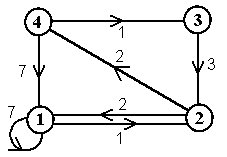
\includegraphics[width=5.5cm,height=3.782cm]{image/a2012Logique2eme-img053.jpg}
		\end{center}

		\begin{center}
			\tablefirsthead{}
			\tablehead{}
			\tabletail{}
			\tablelasttail{}
			\begin{supertabular}{|m{0.40000004cm}|m{0.40000004cm}|m{0.40000004cm}|m{0.40000004cm}|m{0.611cm}|m{0.435cm}|m{0.454cm}|m{0.40000004cm}|m{0.40000004cm}|m{0.486cm}|m{0.435cm}|m{0.58cm}|m{0.40000004cm}|m{0.537cm}|m{0.56200004cm}|m{0.52000004cm}|m{0.435cm}|m{0.435cm}|m{0.435cm}|m{0.47400004cm}|m{0.40000004cm}|m{0.40000004cm}|m{0.40000004cm}|m{0.426cm}|}
			\multicolumn{4}{m{2.2cm}}{\centering{ état initial}} &
			\multicolumn{1}{m{0.611cm}}{~
			} &
			\multicolumn{4}{m{2.289cm}}{\centering{ k=1}} &
			\multicolumn{1}{m{0.486cm}}{~
			} &
			\multicolumn{4}{m{2.5519998cm}}{\centering{ k=2}} &
			\multicolumn{1}{m{0.56200004cm}}{~
			} &
			\multicolumn{4}{m{2.425cm}}{\centering{ k=3}} &
			\multicolumn{1}{m{0.47400004cm}}{~
			} &
			\multicolumn{4}{m{2.226cm}}{\centering{ k=4}}\\\hhline{----~----~----~----~----}
			\centering{ 7} &
			\centering{ 1} &
			\centering{ ${\infty}$} &
			\centering{ ${\infty}$} &
			~
			 &
			\centering{ 7} &
			\centering{ 1} &
			\centering{ ${\infty}$} &
			\centering{ ${\infty}$} &
			~
			 &
			\centering{ 3} &
			\centering{ 1} &
			\centering{ ${\infty}$} &
			\centering{ 3} &
			~
			 &
			\centering{ 3} &
			\centering{ 1} &
			\centering{ ${\infty}$} &
			\centering{ 3} &
			~
			 &
			\centering{ 3} &
			\centering{ 1} &
			{ 4} &
			\centering\arraybslash{ 3}\\\hhline{----~----~----~----~----}
			\centering{ 2} &
			\centering{ ${\infty}$} &
			\centering{ ${\infty}$} &
			\centering{ 2} &
			~
			 &
			\centering{ 2} &
			\centering{ 3} &
			\centering{ ${\infty}$} &
			\centering{ 2} &
			~
			 &
			\centering{ 2} &
			\centering{ 3} &
			\centering{ ${\infty}$} &
			\centering{ 2} &
			~
			 &
			\centering{ 2} &
			\centering{ 3} &
			\centering{ ${\infty}$} &
			\centering{ 2} &
			~
			 &
			\centering{ 2} &
			\centering{ 3} &
			{ 3} &
			\centering\arraybslash{ 2}\\\hhline{----~----~----~----~----}
			\centering{ ${\infty}$} &
			\centering{ 3} &
			\centering{ ${\infty}$} &
			\centering{ ${\infty}$} &
			~
			 &
			\centering{ ${\infty}$} &
			\centering{ 3} &
			\centering{ ${\infty}$} &
			\centering{ ${\infty}$} &
			~
			 &
			\centering{ 5} &
			\centering{ 3} &
			\centering{ ${\infty}$} &
			\centering{ 5} &
			~
			 &
			\centering{ 5} &
			\centering{ 3} &
			\centering{ ${\infty}$} &
			\centering{ 5} &
			~
			 &
			\centering{ 5} &
			\centering{ 3} &
			{ 6} &
			\centering\arraybslash{ 5}\\\hhline{----~----~----~----~----}
			\centering{ 7} &
			\centering{ ${\infty}$} &
			\centering{ 1} &
			\centering{ ${\infty}$} &
			~
			 &
			\centering{ 7} &
			\centering{ 8} &
			\centering{ 1} &
			\centering{ ${\infty}$} &
			~
			 &
			\centering{ 6} &
			\centering{ 8} &
			\centering{ 1} &
			\centering{ 10} &
			~
			 &
			\centering{ 6} &
			\centering{ 4} &
			\centering{ 1} &
			\centering{ 6} &
			~
			 &
			\centering{ 6} &
			\centering{ 4} &
			{ 1} &
			\centering\arraybslash{ 6}\\\hhline{----~----~----~----~----}
			\end{supertabular}
		\end{center}

		\textbf{Remarque.} L'algorithme ci-dessus détermine les poids 
		minimum entre toutes les paires de n{\oe}uds du graphe. Il existe
		de nombreuses variantes, dont l'\textbf{algorithme de Dijkstra} 
		qui recherche les poids uniquement entre un n{\oe}ud
		donné et les autres n{\oe}uds du graphe. Cet algorithme utilise 
		seulement un tableau de $n$ valeurs (au lieu d'une matrice $n$ x $n$).

	\subsection{Parcours d'un graphe}
	%================================
		
		Comment parcourir les n{\oe}uds d'un graphe ? Plusieurs solutions sont 
		possibles. On pourrait bien sûr les parcourir dans l'ordre de leur 
		énumération, mais ce parcours ne tiendrait pas compte des liens 
		entre les n{\oe}uds. Deux parcours particuliers apparaissent dans 
		la théorie des graphes, selon le type de problème à résoudre~: 
		le parcours \textit{par contagion} et le parcours \textit{par sondage}.

		Au cours de l'exécution des algorithmes correspondant à ces parcours, 
		chaque n{\oe}ud sera dans un des 3 états suivants~: 
		\textbf{Prêt} (état initial), \textbf{Attente }(en attente d'être traité) 
		ou \textbf{Traité}.

		Ces états peuvent être stockés dans un tableau de chaines, 
		ou éventuellement de booléens (en assimilant les états
		\textbf{Attente} et \textbf{Traité} en un seul état 
		«~\textbf{Visité}~»). Dans les deux algorithmes ci-dessous, 
		la détermination des n{\oe}uds voisins est très aisée, que 
		ce soit par la matrice d'adjacence ou par le tableau de listes.
		Les algorithmes sont rédigés en «~macro-logique~», afin de 
		pouvoir les adapter facilement selon le choix de la
		représentation choisie.

		\subsubsection{Parcours par contagion}
		%=====================================
			
			À partir d'un n{\oe}ud de départ, on visite d'abord ses voisins, 
			puis les voisins des voisins et ainsi de suite, ...
			On visite donc le graphe par «~couches~», d'abord les voisins 
			dans l'entourage immédiat, puis on s'éloigne petit à
			petit de plus en plus loin...

			\cadre{
				\begin{pseudo}
					\Module{ParcoursContagion}{départ, ...}{} 
					\RComment la représentation du graphe n'est pas précisée ici
						\LComment initialiser tous les états des n{\oe}uds à prêt
						\Let état de départ \Gets Attente
						\Stmt file.enfiler(départ)
						\While{NON file.estVide( )}
							\Let n{\oe}ud \Gets file.défiler( )
							\LComment traitement du n{\oe}ud
							\Let état de n{\oe}ud \Gets Traité
							\For{tous les voisins de n{\oe}uds}
								\If{état de voisin = Prêt}
									\Let état de voisin \Gets Attente
									\Stmt file.enfiler(voisin)
								\EndIf
							\EndFor
						\EndWhile
					\EndModule
				\end{pseudo}
			}
			
		\subsubsection{Parcours par sondage}
		%===================================
			
			L'algorithme est semblable au précédent, à part que l'on 
			utilise ici une pile au lieu d'une file. Il en résulte le
			parcours suivant~: à partir du n{\oe}ud de départ, on 
			visite un voisin, puis immédiatement un voisin de ce voisin et
			ainsi de suite, on s'éloigne le plus loin possible jusqu'à un 
			premier cul-de-sac. On revient alors en arrière et on
			recommence dans la première voie non encore visitée.

			\cadre{
				\begin{pseudo}
					\Module{ParcoursSondage}{départ, ...}{}
					\RComment la représentation du graphe n'est pas précisée ici
						\LComment initialiser tous les états des n{\oe}uds à prêt
						\Let état de départ \Gets Attente
						\Stmt pile.empiler(départ)
						\While{NON pile.estVide( )}
							\Let n{\oe}ud \Gets pile.dépiler( )
							\LComment traitement du n{\oe}ud
							\Let état de n{\oe}ud \Gets Traité
								\For{tous les voisins de n{\oe}uds}
									\If{état de voisin = Prêt}
										\Let état de voisin \Gets Attente
										\Stmt pile.empiler(voisin)
									\EndIf
								\EndFor
							\EndWhile
						\EndModule
					\end{pseudo}
				}

			\textbf{Remarque.} Noter que dans ces algorithmes, il n'y a pas 
			de contrainte sur l'ordre de visite des voisins, celui-ci
			dépendra en partie de l'énumération des n{\oe}uds 
			choisie ou du parcours des listes d'adjacence.

			\textbf{Exemple~:} Dans le graphe suivant, en supposant que les 
			voisins soient parcourus dans l'ordre des listes du tableau, le
			parcours par contagion à partir de A donnera A, D, E, B, C et 
			le parcours par sondage A, E, D, C, B.

			\begin{center}
			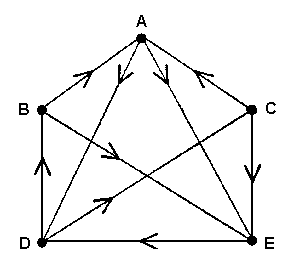
\includegraphics[width=4.99cm,height=4.473cm]{image/a2012Logique2eme-img054.png}  \ \ \ \ \ \ \ \ \ \ \ \ \ 
			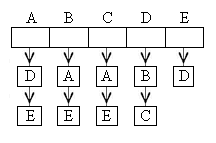
\includegraphics[width=5.715cm,height=3.784cm]{image/a2012Logique2eme-img055.png} 
			\end{center}


%==================
\section{Exercices}
%==================

	\begin{Exercice}{}
		Soit un graphe orienté dont la matrice d'adjacence est la suivante~:
				
		\begin{center}
			\tablefirsthead{}
			\tablehead{}
			\tabletail{}
			\tablelasttail{}
			\begin{supertabular}{m{0.93900007cm}|m{0.81600004cm}|m{0.81600004cm}|m{0.81600004cm}|m{0.81600004cm}|m{0.81600004cm}|}
			\multicolumn{1}{m{0.93900007cm}}{~
			} &
			\multicolumn{1}{m{0.81600004cm}}{\centering{ A}} &
			\multicolumn{1}{m{0.81600004cm}}{\centering{ B}} &
			\multicolumn{1}{m{0.81600004cm}}{\centering{ C}} &
			\multicolumn{1}{m{0.81600004cm}}{\centering{ D}} &
			\multicolumn{1}{m{0.81600004cm}}{\centering\arraybslash{ E}}\\\hhline{~-----}
			\centering{ A} &
			\centering{ F} &
			\centering{ V} &
			\centering{ F} &
			\centering{ V} &
			\centering\arraybslash{ F}\\\hhline{~-----}
			\centering{ B} &
			\centering{ F} &
			\centering{ F} &
			\centering{ V} &
			\centering{ F} &
			\centering\arraybslash{ F}\\\hhline{~-----}
			\centering{ C} &
			\centering{ V} &
			\centering{ F} &
			\centering{ F} &
			\centering{ F} &
			\centering\arraybslash{ F}\\\hhline{~-----}
			\centering{ D} &
			\centering{ F} &
			\centering{ F} &
			\centering{ F} &
			\centering{ F} &
			\centering\arraybslash{ V}\\\hhline{~-----}
			\centering{ E} &
			\centering{ V} &
			\centering{ F} &
			\centering{ F} &
			\centering{ F} &
			\centering\arraybslash{ F}\\\hhline{~-----}
			\end{supertabular}
		\end{center}
		
		\begin{enumerate}
			\item {
				Dessiner le graphe correspondant}
			\item {
				Établir la matrice d'accessibilité par l'algorithme de Roy-Warshall}
			\item {
				Que représente la matrice obtenue à la 3\textsuperscript{ème} étape de cet algorithme ?}
		\end{enumerate}
		
	\end{Exercice}
	
	\begin{Exercice}{}
		Un graphe orienté est représenté par un tableau de 
		listes d'adjacence. Le contenu de ce tableau est
		(2), ( ), (1,3), (2, 4), (3, 5, 7), (4, 6), (5, 7), (4, 6). 
		Dessiner un graphe correspondant.

	\end{Exercice}
	
	\begin{Exercice}{}
		Soit le graphe orienté suivant~:
		
		\begin{center}
		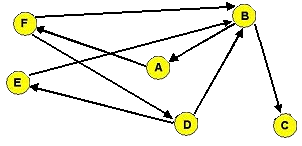
\includegraphics[width=6.854cm,height=3.318cm]{image/a2012Logique2eme-img056.png}
		\end{center}

		\begin{itemize}
			\item {
				Donner sa matrice d'adjacence, en faisant correspondre les lettres 
				prises dans l'ordre alphabétique aux indices pris
				dans l'ordre croissant.}
			\item {
				Ce graphe est-il complet? Expliquer.}
			\item {
				Ce graphe contient-il des n{\oe}uds particuliers? Si oui, lesquels.}
			\item {
				Existe-t-il un chemin reliant B à E ? Si oui lequel. 
				Dans quelle étape de l'algorithme de Roy-Warshall ce chemin
				apparait-il ? }
			\item {
				Que donne l'énumération des valeurs des n{\oe}uds donnée 
				par contagion à partir du n{\oe}ud F ? }
			\item {
				Même question par sondage.}
		\end{itemize}

	\end{Exercice}
	
	\begin{Exercice}{}
		Soit un graphe orienté à $n$ n{\oe}uds (avec $n>1$). 
		Comment relier ces n{\oe}uds avec le nombre minimum d'arcs pour 
		obtenir un graphe dont la matrice d'accessibilité ne contienne 
		que des 1 ? Quel est le nombre minimum d'arcs requis ?

	\end{Exercice}
	
	\begin{Exercice}{}
		Est-il possible que la matrice d'accessibilité 
		d'un graphe soit identique à sa matrice d'adjacence ?
	\end{Exercice}
	
	\begin{Exercice}{}
		Soit un graphe non orienté donné par sa matrice d'adjacence 
		(a) symétrique (b) triangulaire supérieure. 
		Écrire un algorithme qui détermine le n{\oe}ud de plus grand 
		degré de ce graphe. En cas d'ex-æquo, on retournera le n{\oe}ud de
		plus petit indice.

	\end{Exercice}
	
	\begin{Exercice}{}
		Soit un graphe non orienté donné par sa matrice d'adjacence. 
		Écrire un algorithme qui détermine le nombre de
		sous-composantes connexes de ce graphe. \
		Même question pour un graphe orienté.

	\end{Exercice}
	
	\begin{Exercice}{}
		Soit un graphe orienté donné par sa matrice d'adjacence 
		($n$ \textsf{x} $n$). Écrire un algorithme qui établit la représentation 
		de ce graphe par un tableau de listes d'entiers (a) de la classe Liste 
		(b) de la classe ListeChainée.

	\end{Exercice}
	
	\begin{Exercice}{}
		Problème inverse~: soit un graphe orienté donné par un tableau 
		de listes chainées d'entiers, écrire un algorithme qui
		détermine la matrice d'adjacence de ce graphe.

	\end{Exercice}
	
	\begin{Exercice}{}
		Écrire un algorithme qui reçoit un entier $n$ 
		en paramètre ($n \geq 3$) et retourne la matrice
		d'adjacence d'un graphe ayant la forme suivante~: 
		le contour est un $n$-gone, et chaque n{\oe}ud est relié à
		ses 4 voisins les plus proches, comme le suggère 
		le dessin suivant dans le cas $n$ = 8.
		\begin{center}
		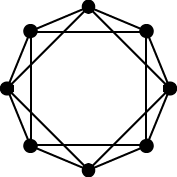
\includegraphics[width=4.073cm,height=4.073cm]{image/a2012Logique2eme-img057.png}
		\end{center}

	\end{Exercice}
	
	\begin{Exercice}{}
		Pour un graphe orienté donné par un tableau de listes d'adjacence, 
		écrire un algorithme qui détermine le n{\oe}ud de
		degré maximum. En cas d'ex-æquo, on retournera le n{\oe}ud 
		de plus petit indice.

	\end{Exercice}
	
	\begin{Exercice}{}
		Soit un graphe orienté donné par sa matrice d'adjacence. 
		Écrire un algorithme qui détermine le nombre de puits du
		graphe. \ Même question avec les sources.

	\end{Exercice}
	
	\begin{Exercice}{}
		Écrire l'algorithme qui calcule la matrice d'accessibilité 
		d'un graphe orienté par la formule de la somme des puissances
		de la matrice d'adjacence. 
		Quelle est la complexité de cet algorithme ? 
		Comparer avec la complexité de l'algorithme de Roy-Warshall.

	\end{Exercice}
	
	\begin{Exercice}{}
		Soit un graphe orienté donné par un tableau de listes (de la classe Liste). 
		Écrire l'algorithme qui permet de parcourir le graphe par contagion 
		à partir d'un n{\oe}ud de départ entré en paramètre. 

	\end{Exercice}
	
	\begin{Exercice}{}
		Soit un graphe orienté donné par un tableau de listes chainées. 
		Écrire l'algorithme qui donne sous la même forme le
		graphe issu de la matrice d'accessibilité du graphe de départ.
		
	\end{Exercice}
	
	\begin{Exercice}{}
		Soit un graphe dont les valeurs attachées aux n{\oe}uds 
		sont contenues dans un tableau valN{\oe}uds de $n$ entiers, 
		et soit $M$ sa matrice d'adjacence (tableau $n$ \textsf{x} $n$ 
		de booléens). Écrire un algorithme qui supprime de ce graphe 
		toutes les arêtes reliant deux n{\oe}uds de valeurs paires.
		
	\end{Exercice}
	
	\begin{Exercice}{}
		Dans un graphe orienté, une \textbf{racine} est un n{\oe}ud 
		à partir duquel on peut atteindre tous les autres n{\oe}uds.
		Écrire un module qui reçoit en paramètre la matrice d'adjacence 
		du graphe et un numéro de n{\oe}ud, et retourne un
		booléen indiquant si ce n{\oe}ud est une racine.

	\end{Exercice}
	
	\begin{Exercice}{}
		Un réseau de métro est composé de plusieurs lignes qui 
		peuvent se croiser en certaines stations. Les lignes sont
		implémentées dans un tableau \textbf{lignes} de listes~: 
		chaque élément du tableau est une liste chainée
		bidirectionnelle contenant les noms des stations dans 
		l'ordre de parcours d'une ligne donnée. Deux stations distinctes
		ont nécessairement des noms différents et une station 
		n'apparait qu'une seule fois pour chaque ligne.

		On demande d'implémenter une classe Réseau, en complétant le code 
		du constructeur et des 3 méthodes décrites ci-dessous~:

		\cadre{
			\begin{pseudo}
				\Class{Réseau}
					\Private 
						\RComment {à vous de donner les éléments privés}
					\Public 
						\ConstrSign{Réseau}{lignes~: tableau [1 à n] de ListeBi<chaine>}
						\MethodSign{getStations}{}{tableau [1 à m] de chaines}
						\LComment retourne le tableau des noms de toutes les stations du réseau
						\MethodSign{getAdjacence}{}{tableau [1 à m, 1 à m] de booléens}
						\LComment {retourne la matrice d'adjacence symétrique du graphe représentant le réseau.
						Chacune des stations est représentée par l'indice 
						que son nom a dans le tableau retourné par getStations( ).}
						\MethodSign{getDistance}{station1, station2~: chaines}{entier}
						\LComment {retourne la matrice des longueurs des chemins les plus courts 
						entre les différentes stations. Ici aussi chacune des stations est 
						représentée par l'indice que son nom a dans le tableau retourné par getStations( ).}
				\EndClass
			\end{pseudo}
		}
		
		\textbf{Remarque~:} on peut supposer que le réseau comporte moins de 
		500 stations et que le réseau est connexe.

	\end{Exercice}
	
	\begin{Exercice}{}
		Implémenter l'interface graphe dont les méthodes sont 
		décrites ci-dessous dans une classe (a) GrapheOrienté 
		(b) GrapheNonOrienté.
		
		\cadre{
			\begin{pseudo}
				\Interface{Graphe<T>}
					\MethodSign{getNbN{\oe}uds( )}{}{entier}
					\MethodSign{ajouteN{\oe}ud}{n{\oe}ud~: T}{}
					\MethodSign{retireN{\oe}ud}{indN{\oe}ud~: entier}{T}
					\MethodSign{setN{\oe}ud}{indN{\oe}ud~: entier, n{\oe}ud~: T}{}
					\MethodSign{getN{\oe}ud}{indN{\oe}ud~: entier}{T}
					\MethodSign{sontAdjacents}{indN{\oe}ud1~: entier, indN{\oe}ud2~: entier}{booléen}
					\MethodSign{getDistance}{indDepart~: entier, indArrivee~: entier}{entier}
					\MethodSign{getAccessibles}{indDepart~: entier, indArrivee~: entier}{booléen}
					\MethodSign{getSondage}{indDepart~: entier}{Liste<entier>}
					\LComment retourne la liste des n{\oe}uds dans l'ordre d'un parcours par sondage
					\MethodSign{getContagion}{indDepart~: entier}{Liste<entier>}
					\LComment retourne la liste des n{\oe}uds dans l'ordre d'un parcours par contagion
				\EndInterface
			\end{pseudo}
		}
		
	\end{Exercice}
	
\appendix
%\include{log1-annexe-parcours-tab}
%\include{log1-annexe-suites}
%\include{log1-annexe-aide-memoire}
\include{log1-fin}
\end{document}
